\chapter{Implementation of a combined PCI-interferometer on \diiid}
\label{ch:Implementation}


\section{Optical-diagnostic access on \diiid}
\label{sec:Implementation:d3d_ports}
\diiid \space provides optical access to its plasmas
through a number of ports, as indicated in
Fig.~\ref{fig:Implementation:d3d_port_locations}.
The ports are labeled according to their
toroidal positions and their sightlines, and
an experimentalist should have at least
a rough familiarity with these conventions.
The toroidal location of a port
is given in degrees clockwise from ``machine north''
when viewing the machine from above
(note that machine north does \emph{not} correspond
to geographic or magnetic north).
The angular separation of adjacent toroidal ports is $15^{\circ}$.
Port sightlines can be vertical or radial.
Ports with vertical (V) sightlines
are labeled sequentially in terms of increasing major radius,
with $V1$ having the smallest major radius and
$V3$ having the largest major radius.
Radial ports (R) have sightlines
that are roughly aligned with the plasma's minor radius, and
they are labeled according to their positions
relative to the plasma midplane:
R0 sits at the plasma midplane,
R+1 and R+2 are the first and second ports
\emph{above} the plasma midplane, respectively, and
R-1 and R-2 are the first and second ports
\emph{below} the plasma midplane, respectively.

\begin{figure}
  \centering
  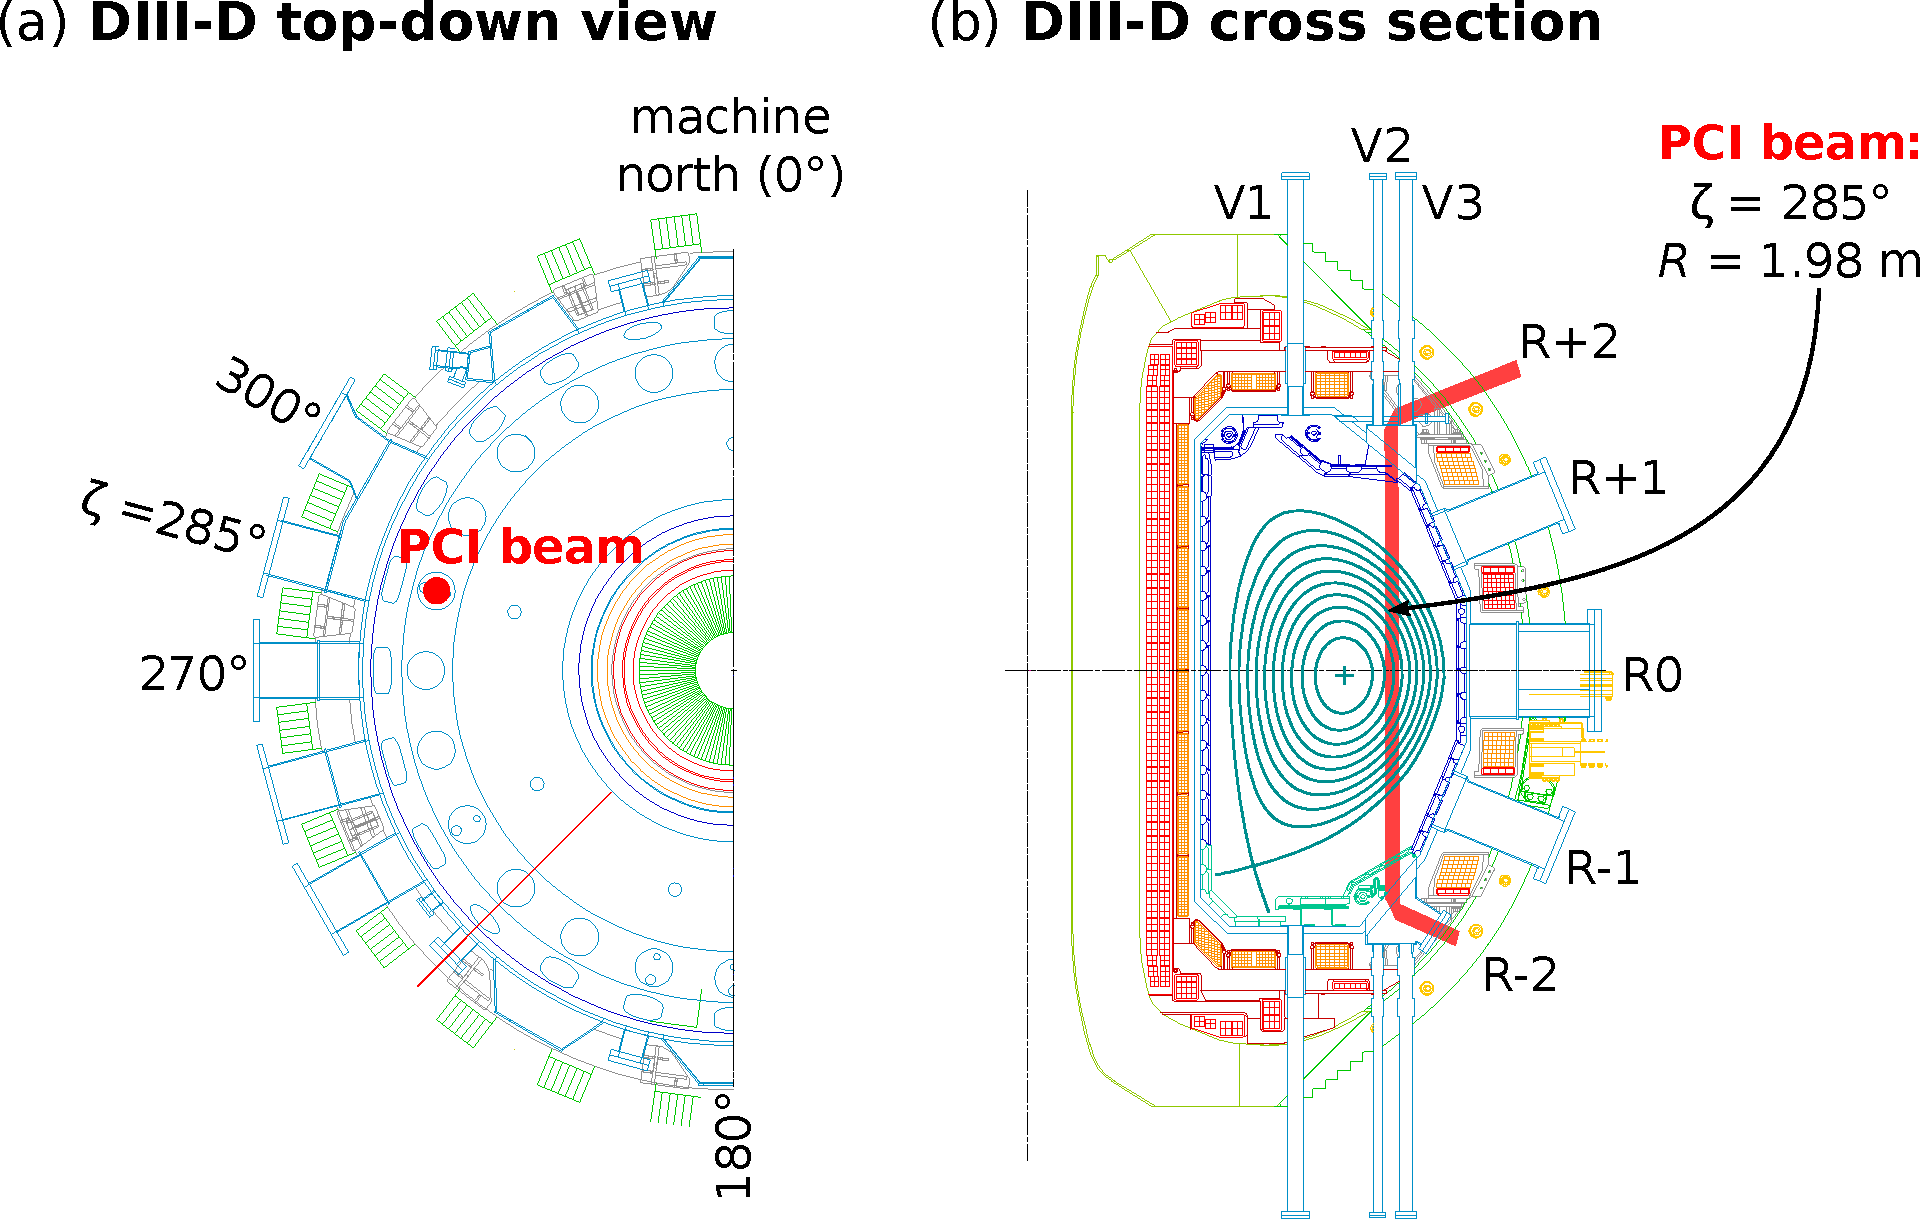
\includegraphics[width = \textwidth]{%
    Chapters/Implementation/figs/d3d_port_locations.pdf}
  \caption[\diiid \space port-labeling conventions and location of PCI]{%
    (a) View of \diiid \space from above,
    indicating the toroidal-labeling convention.
    (b) View of \diiid \space cross section,
    indicating the labeling convention
    for vertical (V) and radial (R) sightlines.
    The PCI beam enters the vessel through the $285^{\circ}$ R+2 port,
    propagates vertically downwards through the plasma
    at a major radius of $R = \SI{1.98}{\meter}$, and
    exits the vessel through the $285^{\circ}$ R-2 port.}
\label{fig:Implementation:d3d_port_locations}
\end{figure}


\section{\diiid's pre-existing PCI system}
\label{sec:Implementation:PCI}
The \diiid \space PCI system is
thoroughly described elsewhere~\cite{dorris_rsi09, dorris_phd}, but
the system components of relevance to this work
are briefly summarized below for completeness.


\subsection{CO$_2$ laser}
\label{sec:Implementation:PCI:laser}
The PCI CO$_2$ laser~\cite[Sec.~3.3]{coda_phd}
has been in service since
the inception of the \diiid\space PCI project in the mid-1990s.
Lasing occurs via high-voltage, DC excitation
inside a $\SI{2}{\meter}$-long, sealed-off glass tube
to produce a TEM$_{00}$ (Gaussian) mode with linear polarization.
The beam waist occurs at the output coupler, and
the corresponding 1/e $E$ radius is $w_0 = \SI{1.25}{\milli\meter}$.
Historically, the laser power has been relatively constant
at $\mathcal{P}_s = \SI{14}{\watt}$, but
the power has declined in the last year.
The laser has
a ``short''-term ($\SI{0.1}{\second}$) peak-to-peak frequency variation
$\lesssim \SI{300}{\kilo\hertz}$ and
a ``long''-term ($\SI{e3}{\second}$) peak-to-peak frequency variation
$\lesssim \SI{3}{\mega\hertz}$;
unfortunately, without knowledge of the corresponding bandwidth,
it is impossible to characterize the laser's phase noise.
A ceiling on the laser phase noise is empirically established in
\textcolor{red}{Section XXX}.


\subsection{System geometry}
\label{sec:Implementation:PCI:geometry}
The system is currently configured
in the ``Phase II'' geometry~\cite{dorris_rsi09},
with the probe beam propagating vertically downwards
from the $285^{\circ}$ R+2 port to the $285^{\circ}$ R-2 port.
The beam center sits at $R = $ \SI{1.98}{\meter}.
Both the toroidal and radial positions
of the PCI beam are shown in
Fig.~\ref{fig:Implementation:d3d_port_locations}.

The PCI system's vertical beam path constrains
the types of fluctuations it can and cannot detect.
Namely, the PCI-measured intensity fluctuations
(\ref{eq:InterferometricMethods:pci_intensity})
correspond to \emph{line-integrated} electron-density fluctuations, which
are the physical origin of the phase fluctuations $\tilde{\phi}$ in
(\ref{eq:InterferometricMethods:phase_fluctuation}).
Because it is a line-integrated measurement,
only fluctuations propagating perpendicular to the beam path are detected,
as fluctuations propagating parallel to the beam path
are effectively averaged out of the signal
\graffito{\textcolor{red}{what about $\delta \omega$?}}
(and, at a more fundamental level, fluctuations propagating
parallel to the beam path do \emph{not} spatially scatter the probe beam).
\graffito{\textcolor{red}{citation? Wesson?}}
Now, electrostatic turbulence (e.g.\ ITG, ETG) tends to be field-aligned
such that $k_{\perp} \gg k_{||}$, where
the $\perp$ and $||$ subscripts are used here to indicate
orientations that are perpendicular to and parallel to
the local magnetic field, respectively.
To lowest order, then, electrostatic fluctuations propagate
perpendicular to a tokamak's toroidal field.
PCI's vertical beam path and
the field-aligned constraint of electrostatic turbulence
imply that PCI is predominantly sensitive to fluctuations
with finite major-radial wavenumber $k_R$.
Thus, PCI's 32-element, 1-dimensional detector array
is oriented in the image plane such that
each detector element corresponds to a unique major radius in the plasma.

In some situations, spatially filtering ``masks''
\cite{dorris_rsi09, dorris_phd, lin_rsi06} or
2-dimensional detector arrays
\cite{sanin_rsi04, tanaka_rsi16}
can be used to localize measurements
by exploiting the spatial variation
in the magnetic field's orientation along the beam path.
These localization techniques typically work best
for high-$k$ measurements.
Note that $k_R$ is related to the
theoretically relevant poloidal wavenumber $k_{\theta}$ via
\begin{equation}
  k_R = k_{\theta} \csc[\alpha(R, z)],
  \label{eq:Implementation:kR_to_ktheta}
\end{equation}
where $\alpha(R, z)$ is the angle
between the beam path and the local flux surface,
as shown schematically in
Fig.~\ref{fig:Implementation:relating_kR_to_ktheta}.
Of course, the fluctuation measurements must be localized,
either via direct measurement
(with 2-dimensional detector arrays or ``masks'')
or via inference from other plasma properties,
before (\ref{eq:Implementation:kR_to_ktheta})
can be inverted to yield $k_{\theta}$
from measured values of $k_R$.

\begin{figure}
  \centering
  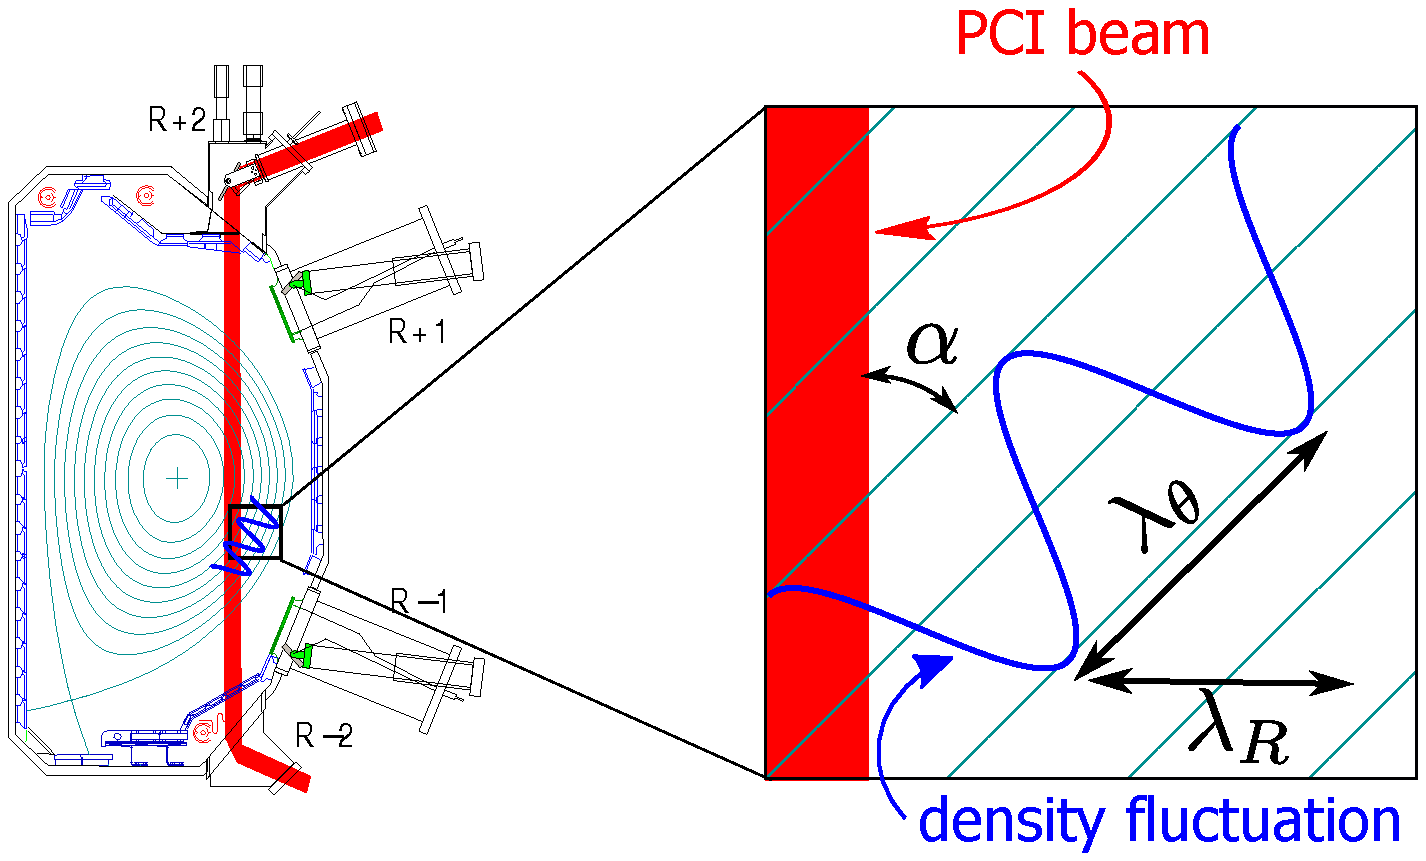
\includegraphics[width = 0.9 \textwidth]{%
    Chapters/Implementation/figs/kR_to_ktheta.pdf}
  \caption[Relating $k_R$ to $k_{\theta}$]{%
    The major-radial wavenumber $k_R = 2 \pi / \lambda_R$ and
    the poloidal wavenumber $k_{\theta} = 2 \pi / \lambda_{\theta}$
    are related via $\alpha(R, z)$, which
    is the angle between PCI's vertical probe beam and
    the local flux surface.}
\label{fig:Implementation:relating_kR_to_ktheta}
\end{figure}


\subsection{Spatial bandwidth}
\label{sec:Implementation:PCI:spatial_bandwidth}
Several critical wavenumbers were defined in
Section~\ref{sec:InterferometricMethods:pci} that
characterize the spatial bandwidth of a PCI system.
The goal of this section is to evaluate each of these
wavenumbers with the relevant parameters from
the \diiid \space PCI system.

PCI's low-$k$ cutoff, $k_g$, is physically constrained by
the free-space diffraction of the in-vessel probe beam.
This constraint was derived both
by examining the far-field overlap of the scattered and unscattered beams as in
(\ref{eq:InterferometricMethods:kmin_for_far_field_beam_separation}) and
by matching the focal-plane spot size of the unscattered beam
with the width of the phase-plate groove as in
(\ref{eq:InterferometricMethods:pci_kmin_physics}).
Both approaches yield the identical constraint that
$k_g^{\text{min}} = 2 / w_0$, where
$w_0$ is the 1/e $E$ radius of the in-vessel probe beam.
The maximum value of $w_0$ is set by the aperture diffraction criterion
(\ref{eq:DesignConsiderations:summary:aperture_radius_for_minimal_diffraction}).
After beam expansion and collimation,
the $4"$-diameter $285^{\circ}$ R+2 port window
is the smallest aperture seen by the beam
prior to its interaction with the plasma.
To satisfy the aperture diffraction criterion
(\ref{eq:DesignConsiderations:summary:aperture_radius_for_minimal_diffraction})
with this $4"$-diameter window,
the expansion optics are configured to produce a collimated beam with
$w_0 = 4/3" \approx \SI{3.4}{\centi\meter}$,
corresponding to
\begin{equation}
  k_g^{\text{min}} \approx \SI{0.6}{\per\centi\meter}.
  \label{eq:Implementation:kg_min}
\end{equation}

PCI's \emph{realized} low-$k$ cutoff, however,
is typically $\sim 2-3 \times$ larger than
the diffraction-limited $k_g^{\text{min}}$.
This occurs if the width of the phase-plate groove is oversized
relative to the unscattered beam's focal-plane spot size.
In such situations the realized low-$k$ cutoff is given by
(\ref{eq:InterferometricMethods:pci_kmin_engineering}).
Despite sacrificing some of the system's low-$k$ range,
operating with an oversized phase-groove width can be advantageous
on large, vibration-prone fusion experiments.
To see this, recall that the phase groove typically reflects
only a fraction $\eta < 1$ of the incident unscattered beam power
(the forward-facing surface of the \diiid\space phase-plate groove
is uncoated ZnSe, which has $\eta = 0.17$ at $\SI{10.6}{\micro\meter}$);
if vibration-induced misalignments
push the unscattered beam out of the phase groove,
there will be large power modulations on the PCI detector
that are \emph{not} attributable to plasma fluctuations and
that push the detector beyond its saturation limits.
While \diiid's PCI system has an elaborate feedback control system
that dynamically centers the unscattered beam on the phase-plate groove
\cite[Sec.~3.5]{coda_phd},
operating with an oversized phase-groove width
gives the feedback system some leeway.
As such, the groove width of the \diiid\space phase plate is
$d = \SI{1}{\milli\meter}$, and
the probe radiation is focused onto the phase plate by
an off-axis parabolic mirror of focal length
$f = 80.7"$ such that the realized low-$k$ cutoff
(\ref{eq:InterferometricMethods:pci_kmin_engineering})
is
\begin{equation}
  k_g \approx \SI{1.5}{\per\centi\meter},
  \label{eq:Implementation:kg_realized}
\end{equation}
approximately $2.5 \times$ larger than
the diffraction-limited minimum in (\ref{eq:Implementation:kg_min}).
Now, for a $\SI{2}{\tesla}$ magnetic field and
a $\SI{1}{\kilo\eV}$ temperature typical of \diiid's pedestal,
a deuteron has a gyroradius $\rho_i \approx \SI{0.3}{\centi\meter}$;
assuming that the PCI beam and the local flux surface
intersect at an angle $\alpha \sim 45^{\circ}$,
(\ref{eq:Implementation:kg_realized})
corresponds to detection of fluctuations from the pedestal with
$k_{\theta} \rho \gtrsim 0.25$.
The higher-temperature core has larger $\rho_i$ but
also typically has smaller $\alpha$, so
the corresponding $k_{\theta} \rho_i$ cutoff in the core
depends on the details
of the temperature profile and the magnetic equilibrium.

PCI's high-$k$ limits are dictated by
finite collection-optic size and system magnification.
The \diiid\space phase plate has a diameter $D = 2"$
such that the phase plate's high-$k$ cutoff
(\ref{eq:InterferometricMethods:pci_kmax_engineering}) is
\begin{equation}
  k_D \approx \SI{75}{\per\centi\meter}.
  \label{eq:Implementation:kD}
\end{equation}
Although the $5"$ diameter $285^{\circ}$ R-2 exit window and
the subsequent $12"$ diameter steering mirrors
are large enough to accommodate beams scattered
from fluctuations with wavenumbers $|k| \sim k_D$,
apertures in the imaging optics
only allow beams scattered from fluctuations with
\begin{equation}
  |k| \lesssim \SI{20}{\per\centi\meter}
\end{equation}
to reach the PCI detector.
Upon reaching the detector,
the measured PCI signal is subject to finite sampling-volume effects,
which result from spatial averaging over the face of a detector element.
The PCI's 32-element, 1-dimensional detector array has elements
of height $\SI{1}{\milli\meter}$,
width $s_x^{\text{pci}} = \SI{0.5}{\milli\meter}$, and
center-to-center element spacing of $\SI{0.55}{\milli\meter}$.
\graffito{\textcolor{red}{Correct? Sign?}}
Coupled with the system's magnification $|M^{\text{pci}}| \approx 0.5$,
the finite sampling-volume cutoff
(\ref{eq:DesignConsiderations:finite_sampling_volume_cutoff})
of the PCI is
\begin{equation}
  k_{\text{fsv}}^{\text{pci}} \approx \SI{63}{\per\centi\meter}.
  \label{eq:Implementation:kfsv_pci}
\end{equation}


\subsection{Temporal bandwidth}
\label{sec:Implementation:PCI:temporal_bandwidth}
PCI's detector ({MCT-$16$-$32$}, Infrared Associates; Stuart, FL USA) and
its associated preamplifiers (also through Infrared Associates)
are the dominant constraint on the system's temporal bandwidth.
The HgCdTe detector array
operates in the photoconductive regime and
is cooled by liquid nitrogen;
the liquid-nitrogen cooling reduces noise and boosts the response such that
the detector-preamplifier combination has
a specific detectivity
$D^* \approx \SI{2e10}{\centi\meter \sqrt\hertz \per\watt}$ and
a $\SI{500}{\volt\per\watt}$ responsivity
to incident $\SI{10.6}{\micro\meter}$ light
(note that the detector also has a saturation intensity
$I_{\text{sat}} \sim \SI{1}{\milli\watt \per\milli\meter\squared}$).
The benefits of cooling, however, come at the expense of reduced bandwidth:
the detector-preamplifier combination has
a high-frequency, $2$-pole cutoff
at $\sim \SI{800}{\kilo\hertz}$~\cite{rost_pci_detector_response}.
As the DC PCI signal is of little interest,
the detector-preamplifier combination also has
a low-frequency, $1$-pole cutoff
at $\sim \SI{2}{\kilo\hertz}$~\cite{rost_pci_detector_response}.

The components downstream of the detector and preamplifiers
have a small impact on the system bandwidth, but
they are briefly summarized below for completeness.
The Variable Gain and Filter (VGAF) circuits~\cite[Sec.~3.3.3]{dorris_phd}
are located immediately downstream of the preamplifiers and
have a low-frequency, $1$-pole cutoff that can be easily switched between
$\SI{10}{\kilo\hertz}$ and $\SI{100}{\kilo\hertz}$;
the VGAFs are typically operated in the $\SI{10}{\kilo\hertz}$ configuration.
Following the VGAFs,
fiber optic links ({$732$ T/R-$2.5$-$33$k}, Analog Modules; Longwood, FL USA)
with an analog bandwidth of DC to $\SI{10}{\mega\hertz}$
transmit the signal from the \diiid\space pit to the annex for digitization.


\subsection{Digitizer}
\label{sec:Implementation:PCI:digitizer}
Upon reaching the annex,
the PCI signals are digitized with two
{ACQ$216$CPCI} boards (D-tAcq Solutions Ltd.; Glasgow, Scotland UK).
The digitizer boards have bit depth $N_b = 14$,
dynamic range $V_{\text{dyn}} = \SI{8}{\volt}$, and
input impedance $Z_{\text{in}} = \SI{50}{\ohm}$.
The digitizer sampling rate is typically $f_s = 4 \, \text{MSPS}$.


\section{Optical layout of heterodyne interferometer}
\label{sec:Implementation:OpticalLayout}
The optical layout of a heterodyne interferometer
sets the interferometer's wavenumber response,
governs the injection of laser phase noise
into the interferometer's measurements, and
influences the interferometer's sensitivity
to vibration-induced misalignment and
small uncertainties in component placement.
Having reviewed the spatial bandwidth
of the pre-existing PCI system in
Section~\ref{sec:Implementation:PCI:spatial_bandwidth},
a complementary spatial bandwidth is selected
for the heterodyne interferometer in
Section~\ref{sec:Implementation:OpticalLayout:spatial_bandwidth}, and
the resulting imaging-system requirements are discussed
in \ref{sec:Implementation:OpticalLayout:element_size}.
Section~\ref{sec:Implementation:OpticalLayout:coalignment_with_feedback}
demonstrates that a carefully designed imaging system and
the PCI focal-plane feedback system can synergistically act
to dynamically maintain the coalignment of the interferometer beams
in the presence of machine vibrations.
Finally,
Sections~\ref{sec:Implementation:OpticalLayout:reference_beam_generation}
and \ref{sec:Implementation:OpticalLayout:probe_beam}
discuss the generation
of the interferometer's reference beam and probe beam and
examine the sensitivity
of the resulting interference signal to small uncertainties
in the placement of the imaging optics.


\subsection{Desired spatial bandwidth}
\label{sec:Implementation:OpticalLayout:spatial_bandwidth}
Because of its external reference beam, a heterodyne interferometer
has a minimum detectable wavenumber of $k = 0$.
This ability to detect fluctuations
below the PCI low-$k$ cutoff (\ref{eq:Implementation:kg_realized})
was one of the primary motivations
for the addition of a heterodyne interferometer
to \diiid's pre-existing PCI system.
Assuming negligible aperture diffraction
(criterion (\ref{eq:DesignConsiderations:summary:aperture_radius_for_minimal_diffraction})),
finite sampling-volume effects govern the wavenumber dependence
of a heterodyne interferometer's transfer function
(\ref{eq:DesignConsiderations:summary:heterodyne_interferometer_wavenumber_transfer_function}),
producing the finite sampling-volume cutoff
(\ref{eq:DesignConsiderations:summary:finite_sampling_volume_cutoff}).
Through careful selection of both
the linear size $s_x$ of the detector element
and the magnification $M$ of the imaging system,
the finite sampling-volume cutoff can be engineered
to provide any desired degree of overlap
with the PCI wavenumber domain.
Producing a reasonable degree of overlap with the PCI and
ensuring that the finite sampling-volume effect
(rather than aperture diffraction)
governs the high-$k$ response
leads naturally to the design point for
the heterodyne interferometer's finite sampling-volume cutoff
\begin{equation}
  k_{\text{fsv}}^{\text{het}} = \SI{5}{\per\centi\meter}.
  \label{eq:Implementation:kfsv_interferometer_design}
\end{equation}
The heterodyne interferometer's desired transfer function
is shown relative to the pre-existing PCI's transfer function in
Fig.~\ref{fig:Implementation:transfer_function_comparison}.

\begin{figure}
  \centering
  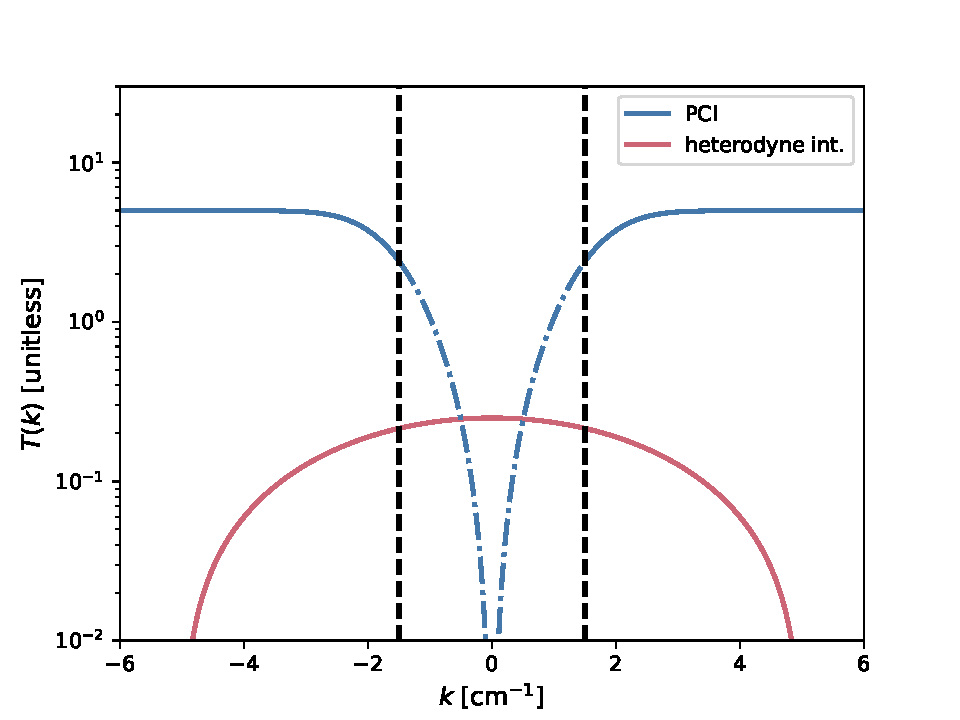
\includegraphics[width = \textwidth]{%
    Chapters/Implementation/figs/transfer_function_comparison.pdf}
  \caption[Design-point wavenumber transfer functions of combined PCI-interferometer]{%
    The design-point wavenumber transfer function
    of the heterodyne interferometer relative to
    that of the pre-existing PCI system.
    The heterodyne interferometer can detect fluctuations from
    $k = 0$ up to its finite sampling-volume cutoff
    (\ref{eq:Implementation:kfsv_interferometer_design}).
    The vertical, dashed lines indicate
    the low-$k$ cutoff of the PCI phase-plate groove,
    $k_g$ from (\ref{eq:Implementation:kg_realized});
    the phase-plate high-$k$ cutoff (\ref{eq:Implementation:kD}) and
    the PCI finite sampling-volume cutoff (\ref{eq:Implementation:kfsv_pci})
    are sufficiently large to negligibly affect the PCI transfer function
    over the depicted wavenumber domain.
    The reflectivity of the PCI phase groove is $\eta = 0.17$.
    Because the PCI transfer function is not defined for $|k| \lesssim k_g$,
    the low-$k$ PCI amplitude response
    (\ref{eq:InterferometricMethods:PCI_amplitude_response})
    is indicated by the dash-dot curves instead.
    The depicted transfer functions should be compared
    to those without finite sampling-volume effects in
    Fig.~\ref{fig:InterferometricMethods:interferometric_method_transfer_functions}.
  }
\label{fig:Implementation:transfer_function_comparison}
\end{figure}


\subsection{Detector-element size}
\label{sec:Implementation:OpticalLayout:element_size}
The heterodyne interferometer's design-point finite sampling-volume cutoff
(\ref{eq:Implementation:kfsv_interferometer_design})
fixes the ratio
of the imaging system's (absolute) magnification $|M|$
to the detector element's linear size $s_x$.
Commercially available detector elements for use at $\SI{10.6}{\micro\meter}$
range in linear size from fractions of a millimeter
to several millimeters~\cite{vigo_catalog}.
Smaller linear element size $s_x$ eases both
the beam-coalignment constraint
(\ref{eq:DesignConsiderations:summary:coalignment_constraint}) and
the curvature-matching constraint
(\ref{eq:DesignConsiderations:summary:radii_of_curvature_matching}).
The variation of detector noise and shot noise
with $s_x$ (but fixed $M / s_x$) can also be examined.
\graffito{\textcolor{red}{Why make this assumption?}}
To proceed, assume that the interferometer image plane
sits in the corresponding Rayleigh range
(i.e.\ $|z_{\image}| \ll z_R$) such that
$w(z_{\image}) \approx |M| w_{\object}$, where
$w(z_{\image})$ is the 1/e $E$ radius of the probe beam at the image plane, and
$w_{\object}$ is the 1/e $E$ radius of the probe beam at the object plane.
The optical power of the probe beam impinging on the detector element is
a function of $s_x / w(z_{\image})$, i.e.\
$P_P = P_P(s_x / w(z_{\image})) \approx P_P(s_x / (|M| w_{\object}))$;
because $M / s_x$ is fixed by the design-point finite sampling-volume cutoff
(\ref{eq:Implementation:kfsv_interferometer_design}),
$P_P$ is also approximately fixed.
The optical power in the reference beam impinging on the detector element,
however, is independent of the magnification and
proportional to the element area $A$, i.e.\ $P_R \propto A$.
Thus, the one-sided autospectral density
of the demodulated detector noise
(\ref{eq:DesignConsiderations:summary:detector_noise_autospectral_density})
is \emph{independent} of the element size.
The one-sided autospectral density
of the demodulated shot noise
(\ref{eq:DesignConsiderations:summary:shot_noise_autospectral_density})
is, in general, a function of the element size;
in the extreme $P_R \gg P_P$,
the spectral density is \emph{independent} of the element size;
in the opposite extreme $P_R \ll P_P$,
the spectral density varies inversely with element area $A$.
In light of the above considerations,
a square detector element of intermediate linear size
\begin{equation}
  s_x = \SI{1}{\milli\meter}
  \label{eq:Implementation:detector_size}
\end{equation}
was chosen.
Referencing the definition of the finite sampling-volume cutoff
(\ref{eq:DesignConsiderations:summary:finite_sampling_volume_cutoff}) and
the interferometer's corresponding design point
(\ref{eq:Implementation:kfsv_interferometer_design}),
it naturally follows that the interferometer imaging system
must have magnification
\begin{equation}
  |M| = 0.08.
  \label{eq:Implementation:magnification_interferometer_design}
\end{equation}


\subsection{Beam coalignment in presence of machine vibrations}
\label{sec:Implementation:OpticalLayout:coalignment_with_feedback}
\diiid's PCI system has an elaborate feedback control system
that dynamically centers the unscattered beam on the phase-plate groove
\cite[Sec.~3.5]{coda_phd}.
Coda has extensively characterized the effect of this feedback system
on the lateral position of the PCI image~\cite[Sec.~3.5(f)]{coda_phd}.
This section extends Coda's analysis by examining
the effect of the feedback system on the misalignment angle $\theta$
between the unscattered probe beam and the image-plane optical axis.
It readily follows from this discussion that,
for certain imaging systems,
the PCI feedback system can dynamically maintain
the beam coalignment
(constraint (\ref{eq:DesignConsiderations:summary:coalignment_constraint}))
of a heterodyne interferometer in the presence of machine vibrations.

First, consider the situation without feedback.
Let the probe beam propagate a distance $l$
from the plasma midplane to a focusing optic with focal length $f$, and
let the focused beam come to a waist a distance $l'$ from the focusing optic.
Now, let a single mirror,
located a distance $d$ upstream from the focusing optic,
be titled away from its nominal position (e.g.\ from machine vibrations),
deflecting the unscattered beam by angle $\beta_1$
relative to the nominal optical axis.
The resulting focal-plane position and orientation of this beam are incorrect
(i.e.\ the beam does not lie on the optical axis, but it should).
This misalignment is depicted by the solid line in
Fig.~\ref{fig:Implementation:feedback_effects}(a).
In a perfectly aligned system,
the focal-plane position and orientation of this beam
would correspond to the ``effective'' beam path
depicted by the dashed line in
Fig.~\ref{fig:Implementation:feedback_effects}(a).
The imaging optics image the object-plane ray
corresponding to this effective beam path.

\begin{figure}
  \centering
  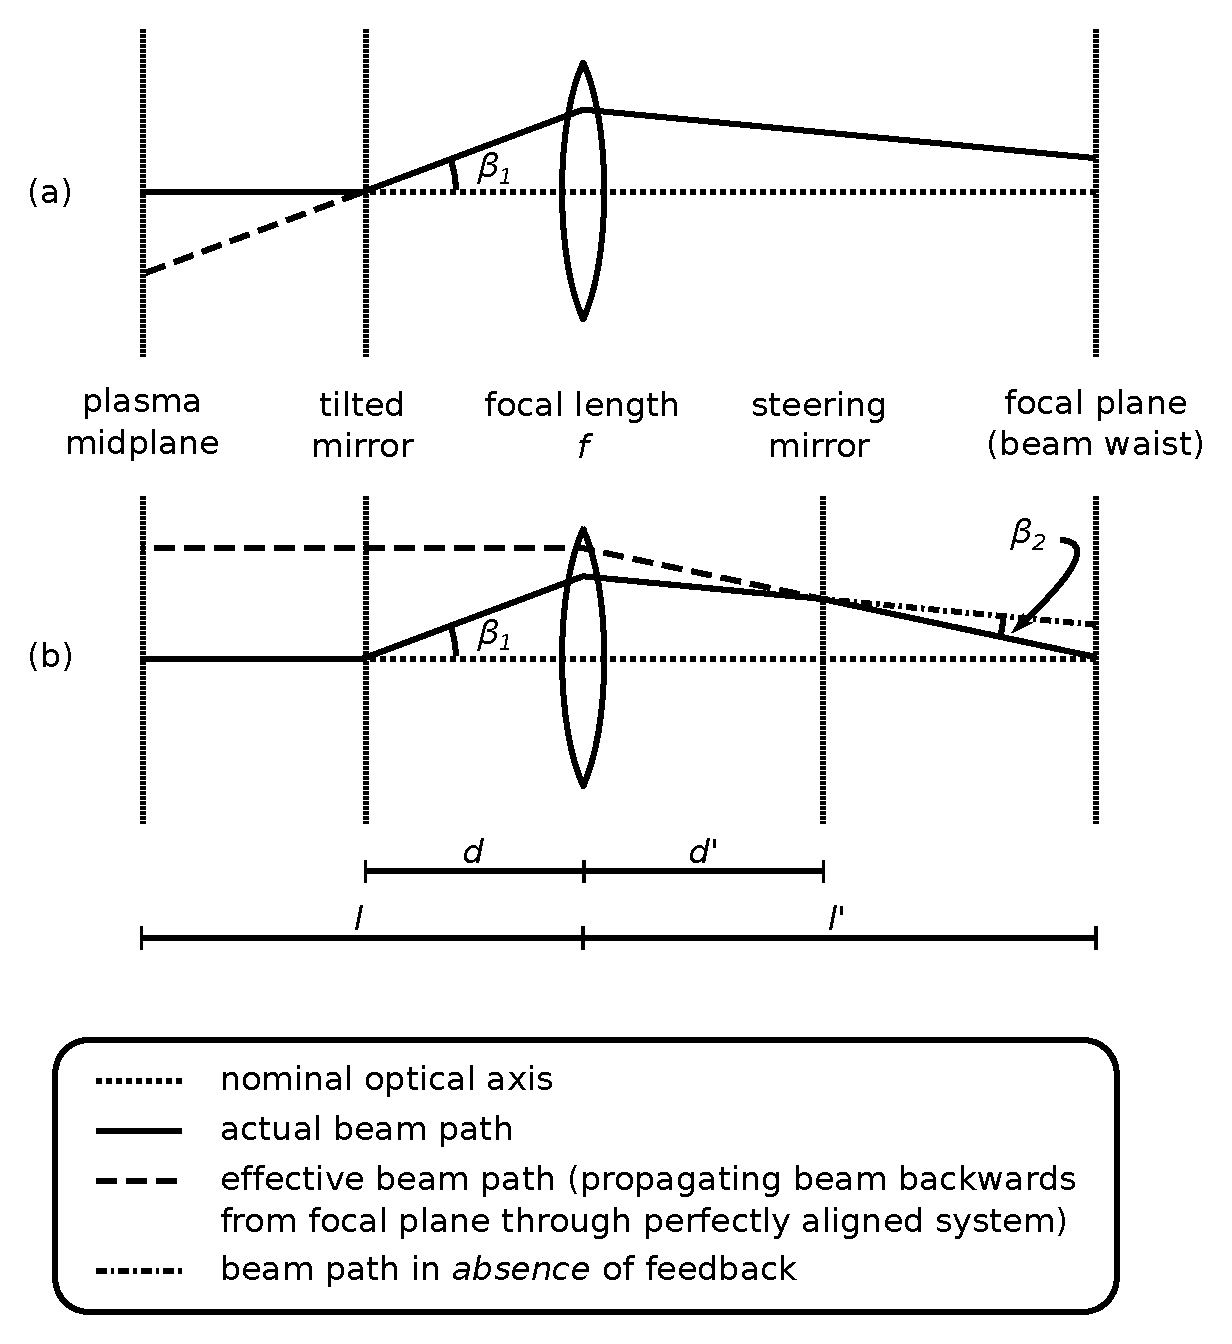
\includegraphics[width = 0.85 \textwidth]{%
    Chapters/Implementation/figs/feedback_effects.pdf}
  \caption[Effect of focal-plane feedback on imaged radiation]{%
    Effect of a tilted mirror
    (a) without focal-plane feedback and
    (b) with focal-plane feedback
    on the actual and effective paths of a Gaussian beam.
    An imaging system images the object-plane ray
    corresponding to the effective beam path.
    Without focal-plane feedback,
    both the transverse distance and the angular orientation
    of the effective object-plane ray are incorrect,
    producing errors in the corresponding image-plane quantities.
    With focal-plane feedback, however,
    the angular orientation of the effective object-plane ray is corrected
    (i.e.\ the ray is parallel to the optical axis,
    albeit laterally displaced);
    then, if the imaging system is engineered
    such that $C = 0$ in the $ABCD$ ray matrix,
    the feedback will dynamically maintain
    the correct angular orientation of the corresponding image-plane ray.
  }
\label{fig:Implementation:feedback_effects}
\end{figure}

Imaging systems are discussed in
Appendix~\ref{app:ImagingSystems}, but
the relevant details are briefly summarized here.
The symmetry axis of a Gaussian beam
behaves as a ray in the geometric-optics sense, where
a ray is fully described by
its transverse distance $\rho$ to the optical axis and
its angular orientation $\theta$ relative to the optical axis.
Ray propagation through a magnification-$M$ imaging system
is well-characterized by an $ABCD$ ray matrix of the form
(\ref{eq:ImagingSystems:ABCD_imaging}).
Specifically,
\begin{align}
  \rho_{\image} &= M \rho_{\object},
  \\
  \theta_{\image} &= \frac{\theta_{\object}}{M} + C \rho_{\object},
\end{align}
where $\object$ indicates object-plane quantities,
$\image$ indicates image-plane quantities, and
$C$ is constant determined by the particulars of the imaging system.
In a perfectly aligned system,
the unscattered beam's object-plane ray
($\rho_{\object} = 0$ and $\theta_{\object} = 0$)
is correctly imaged as $\rho_{\image} = 0$ and $\theta_{\image} = 0$.
However, in a \emph{misaligned} system,
the unscattered beam's \emph{effective} object-plane ray
($\rho_{\object} \neq 0$ and $\theta_{\object} \neq 0$)
is imaged as $\rho_{\image} \neq 0$ and $\theta_{\image} \neq 0$.
Thus, without feedback, a tilted mirror
produces errors in both the image-plane position and orientation
of the unscattered beam.

Now, add a steering mirror a distance $d'$ downstream of the focusing optic.
This steering mirror is tasked with compensating for the titled mirror
by returning the unscattered beam's focal-plane position
to the nominal optical axis,
as depicted in Fig.~\ref{fig:Implementation:feedback_effects}(b).
In the geometric-optics limit,
a ray passing through the intersection of
the optical axis and the focal plane
corresponds to a collimated beam ($\theta = 0$)
upstream of the focusing optic.
Thus, in a perfectly aligned system,
the focal-plane position and orientation
of the feedback-compensated beam
would correspond to the ``effective'' beam path,
depicted by the dashed line in
Fig.~\ref{fig:Implementation:feedback_effects}(b).
Thus, upstream of the focusing optic,
the effective beam path is displaced from but \emph{parallel}
to the nominal optical axis.
As is the case without feedback,
the imaging optics image the object-plane ray
($\rho_{\object} \neq 0$, $\theta_{\object} = 0$)
corresponding to this effective beam path, i.e.\
$\rho_{\image} = M \rho_{\object}$ and
$\theta_{\image} = C \rho_{\object}$.
Thus, for imaging systems with $C = 0$,
the PCI feedback system
will dynamically maintain the correct angular orientation
of the image-plane unscattered beam
(i.e. $\theta_{\image} = 0$);
an obvious application is satisfying
the heterodyne interferometer's coalignment constraint
(\ref{eq:DesignConsiderations:summary:coalignment_constraint})
in the presence of machine vibrations.
Of course, the lateral image location shifts
in accordance with the discussion by Coda~\cite[Sec.~3.5(f)]{coda_phd}.


\subsection{Reference-beam generation}
\label{sec:Implementation:OpticalLayout:reference_beam_generation}
A heterodyne interferometer interferes the imaged probe radiation
with a frequency-shifted reference beam
to make an absolute phase measurement, as discussed in
Section~\ref{sec:InterferometricMethods:interferometry:heterodyne}.
It is easy to Doppler shift $\SI{10.6}{\micro\meter}$ radiation
by tens of $\SI{}{\mega\hertz}$ with an acousto-optic modulator (AOM).
The operation of a typical AOM is described in
in Section~\ref{sec:DesignConsiderations:phase_noise:LO}.

The heterodyne interferometer's reference beam is generated
with a Gooch \& Housego (Ilminster, UK) 37027-5 Germanium AOM,
pictured in Fig.~\ref{fig:Implementation:aom}.
The resonant frequency of the AOM's piezo-actuator
is $\SI{27.12}{\mega\hertz}$, but
the AOM's deflection efficiency varies negligibly
between $\SI{25}{\mega\hertz}$ and $\SI{30}{\mega\hertz}$.
\graffito{\textcolor{red}{As will be discussed\ldots operate at $\SI{30}{\mega\hertz}$}}
For operation at $\Delta f_0 = \SI{30}{\mega\hertz}$,
the deflected beam is separated from the undeflected beam by
$2 \theta_B = \SI{59}{\milli\radian}$, where
$\theta_B$ is the Bragg angle from
(\ref{eq:DesignConsiderations:Bragg_angle}).
Deflection efficiency scales roughly linearly with RF power, and
deflection efficiencies in excess of $75\%$
can be obtained at the maximum-rated RF power of $\SI{30}{\watt}$.
The RF power is CW such that
the AOM simply deflects and Doppler shifts
a fraction of the incident optical beam.
(In contrast, rapidly varying the RF power modulates
the optical powers in the deflected and undeflected beams, but
such modulation is \emph{not} desirable in a heterodyne interferometer).
The AOM's static optical insertion loss is measured to be $\sim 10\%$, and
the incident optical intensity should be limited to
$\leq \SI{5}{\watt\per\milli\meter\squared}$
to avoid thermal lensing of the beam.
The diameter of the piezo-driven acoustic beam is $\sim\SI{5}{\milli\meter}$.
Satisfying both the AOM's peak-intensity constraint and
the aperture-diffraction constraint
(\ref{eq:DesignConsiderations:summary:aperture_radius_for_minimal_diffraction},
with the acoustic beam providing an ``effective aperture'')
requires placement of the AOM $\sim15"$ downstream
of the laser's beam waist.
\graffito{\textcolor{red}{Need a section on source parameters}}

\begin{figure}
  \centering
  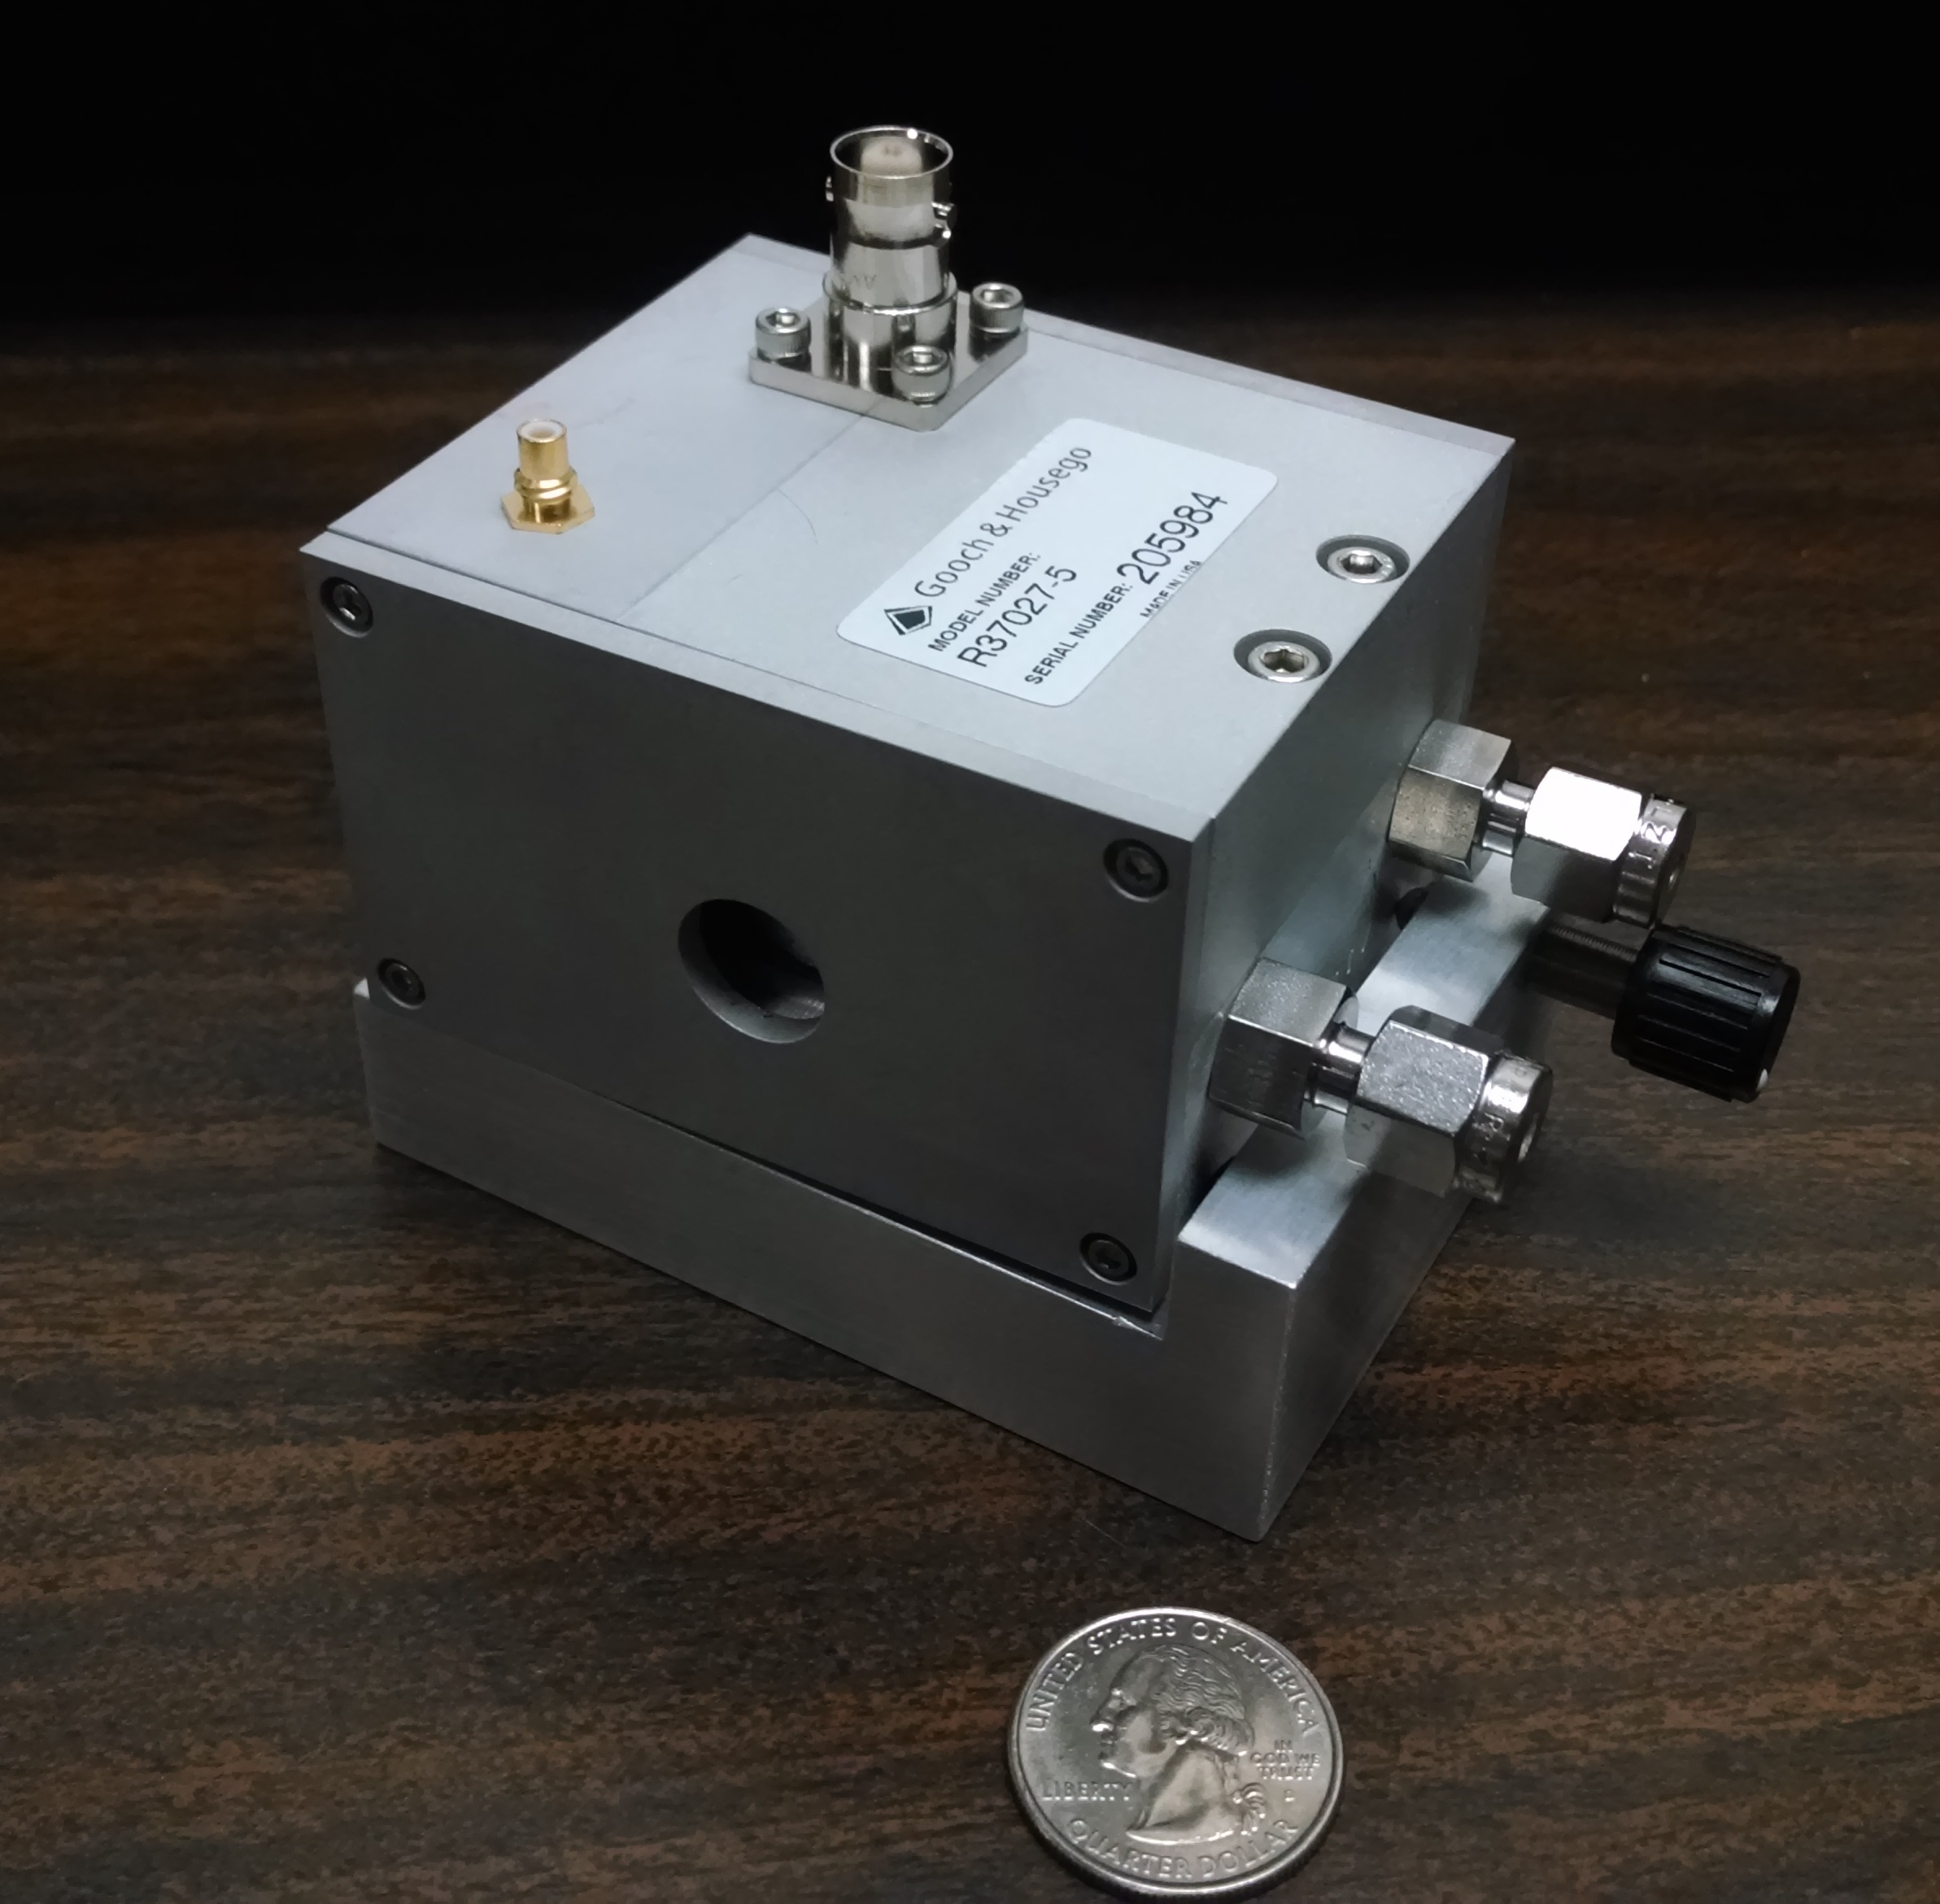
\includegraphics[width = 0.6 \textwidth]{%
    Chapters/Implementation/figs/aom.jpg}
  \caption[Acousto-optic modulator (AOM)]{%
    The heterodyne interferometer's Germanium acousto-optic modulator (AOM).
    The AOM deflects and Doppler shifts ($\Delta f_0 = \SI{30}{\mega\hertz}$)
    a fraction of the incident CO$_2$ beam ($f_0 = \SI{28.3}{\tera\hertz}$)
    to produce a reference beam.
    The $\SI{30}{\mega\hertz}$ RF signal is coupled to the AOM
    through the upper-left BNC jack, and
    the resulting sound waves propagate through the Germanium crystal
    from left to right.
    The CO$_2$ beam enters through the aperture on the AOM's face and
    exits through a similar aperture on the AOM's rear.
    The twin Swagelock fittings on the AOM's right
    provide an inlet and outlet for water cooling, while
    the lower-left SMC jack connects to
    a normally closed, creep-action PEPI N thermostat
    that provides a thermal interlock to the AOM's RF driver.
    The AOM is mounted on a ``Bragg mount'', which
    allows easy optimization of the beam's angle of incidence
    (via the mount's adjustment screw, seen in black at the middle-right).
  }
\label{fig:Implementation:aom}
\end{figure}

Due to space constraints, the reference-beam path length
is \emph{not} matched to the probe-beam path length.
This path-length discrepancy \textcolor{red}{$L \approx \SI{10}{\meter}$}
injects the laser's phase noise
into the heterodyne interferometer's measurements, as quantified by
(\ref{eq:DesignConsiderations:summary:laser_phase_noise_autospectral_density}).
However, as shown in \textcolor{red}{Section~???},
the laser's phase noise negligibly contributes
to the heterodyne interferometer's noise floor.

Allowing such a ``modest'' path-length discrepancy
substantially simplifies the optical design of the reference arm.
Following its generation at the AOM,
the reference beam is directed to the interferometer detector
with four broadband metallic mirrors
(ER.2 protected-silver coated from
Newport Corporation, Irvine, CA USA) and
is combined with the probe beam
via a 50\% reflective, polarization-independent ZnSe beam splitter
(II-VI Infrared, Saxonburg, PA USA).
No lenses are used to condition the reference beam.
However, a multiple-order $\SI{10.6}{\micro\meter}$ half waveplate
(II-VI Infrared, Saxonburg, PA USA)
sits between the AOM and the polarization-independent beam combiner.
As the probe beam is \emph{not} confined to a single plane,
out-of-plane mirror reflections can rotate the probe-beam polarization;
the half waveplate allows one to easily align the polarization
of the reference beam with that of the probe beam,
thereby maximizing the interference signal.
From source to detector, the reference beam
propagates a total distance $59\text{-}3/8"$.


\subsection{Probe-beam generation \& imaging}
\label{sec:Implementation:OpticalLayout:probe_beam}
The heterodyne interferometer and the pre-existing PCI system
\emph{share} the in-vessel probe beam.
The only modification to the beam-generation optics
was the addition of the AOM, discussed extensively in
Section~\ref{sec:Implementation:OpticalLayout:reference_beam_generation}.
The AOM insertion loss and
the diversion of some of the laser power to the reference arm
reduce the power in the probe beam relative to the PCI-only configuration.

As in the PCI system, the probe arm of the heterodyne interferometer
is configured to \emph{image} the probe radiation from the tokamak midplane.
The heterodyne interferometer and PCI imaging optics share
the focusing $f = 80.7"$ off-axis parabolic mirror and
the feedback steering mirrors~\cite[Sec.~3.5]{coda_phd}.
Because the phase plate's spatial filtering
produces the PCI's low-$k$ cutoff,
a $2"$ diameter $S$-polarization ZnSe splitter
(II-VI Infrared, Saxonburg, PA USA)
located $5\text{-}1/8"$ upstream of the phase plate
diverts a fraction of the probe radiation
to dedicated heterodyne-interferometer optics.
\graffito{\textcolor{red}{What fraction??}}
(This beam splitter also diverts a portion of the unscattered probe beam
to the feedback system's quadrant detector;
the heterodyne interferometer's probe beam and
the feedback beam are separated with
an additional $2"$ diameter $S$-polarization ZnSe splitter).
Four broadband metallic mirrors
(ER.2 protected-silver coated from
Newport Corporation, Irvine, CA USA)
direct the probe radiation through the remainder
of the heterodyne interferometer's imaging optics, which
consist of two plano-convex ZnSe lenses
(II-VI Infrared, Saxonburg, PA USA).
The first lens $L1$ has a $7.5"$ focal length and a $2"$ diameter, and
the second lens $L2$ has a $7.5"$ focal length and a $1.5"$ diameter.
Then, under the constraint of imaging the plasma midplane,
the remaining design parameters are
the distance $d_{P2,L1}$ between
the focusing off-axis parabolic mirror and $L1$ and
the distance $d_{L1,L2}$ between $L1$ and $L2$.

% \begin{figure}[h!]
\begin{figure}
  \centering
  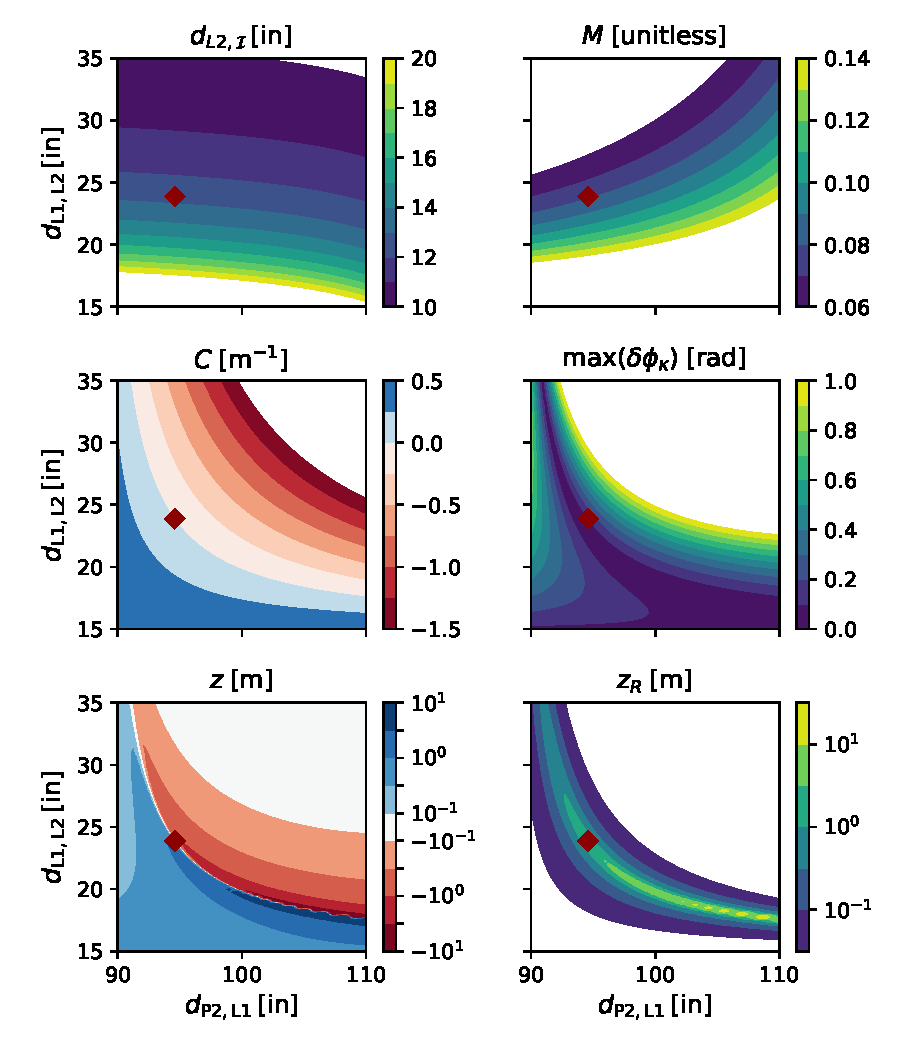
\includegraphics[width = \textwidth]{%
    Chapters/Implementation/figs/optical_design_sensitivity.pdf}
  \caption[Sensitivity of optical design to placement of imaging optics]{%
    Sensitivity of heterodyne-interferometer optical design
    to the placement of lenses $L1$ and $L2$.
    % The distance between the off-axis parabolic mirror $P2$
    % (which focuses the collimated probe beam) and
    % the first lens $L1$ of the imaging system
    % is denoted by $d_{P2,L1}$ (along the $x$-axis), and
    % the distance between $L1$ and the second lens $L2$
    % is denoted by $d_{L1,L2}$ (along the $y$-axis).
    The design point is marked with a burgundy diamond.
    See text for discussion.
  }
\label{fig:Implementation:optical_design_sensitivity}
\end{figure}

The sensitivity of the heterodyne-interferometer optical layout
to $d_{P2,L1}$ and $d_{L1,L2}$ is shown in
Fig.~\ref{fig:Implementation:optical_design_sensitivity}, and
the resulting implications are discussed here in detail.
The \emph{top-left} panel of
Fig.~\ref{fig:Implementation:optical_design_sensitivity} displays
the distance from $L2$ to the image plane $\image$.
The image-plane location is a strong function of $d_{L1,L2}$ and
a weak function of $d_{P2,L2}$.
The \emph{top-right} panel of
Fig.~\ref{fig:Implementation:optical_design_sensitivity} displays
the imaging system's magnification $M$,
with the design point in accord with
(\ref{eq:Implementation:magnification_interferometer_design}).
The magnification is a strong function of $d_{L1,L2}$.
The \emph{middle-left} panel of
Fig.~\ref{fig:Implementation:optical_design_sensitivity} displays
the $C$ parameter of the imaging system's $ABCD$ ray matrix.
As discussed in Section~\ref{sec:Implementation:OpticalLayout:coalignment_with_feedback},
the PCI feedback system will dynamically maintain
the coalignment of the heterodyne interferometer's beams if $C = 0$.
The $C$ parameter is a strong function
of both $d_{P2,L1}$ and $d_{L1,L2}$, and
experimental uncertainties in distances and focal lengths
make it difficult to enforce $C = 0$.
(Indeed, the amplitude of the interference signal from the realized system
\emph{does} vary with vibrations, indicating that
$C \neq 0$ and/or the action of the feedback system is not sufficient
to maintain coalignment).
The \emph{middle-right} panel of
Fig.~\ref{fig:Implementation:optical_design_sensitivity} displays
the maximum curvature-induced phase shift
(\ref{eq:DesignConsiderations:summary:radii_of_curvature_matching})
for a single, $\SI{1}{\milli\meter\squared}$ square detector.
The design point satisfies $\text{max}(\delta \phi_{\kappa}) \ll 1$
such that curvature-induced phase shifts
minimally reduce the interference power and
negligibly distort the imaged wavenumbers.
The \emph{bottom-left} panel of
Fig.~\ref{fig:Implementation:optical_design_sensitivity} displays
the axial distance $z$ from the waist of the probe beam to the image plane
(this is the usual axial parameter used to characterize Gaussian beams, with
$z > 0$ indicating that the waist is upstream of the image plane and
$z < 0$ indicating that the waist is downstream of the image plane).
There is only a very narrow strip
where the image plane and the beam waist coincide
(i.e.\ where $z = 0$);
note that this strip closely resembles
the $C = 0$ curve of the middle-left panel.
This is no coincidence:
as discussed in the text surrounding
(\ref{eq:ImagingSystems:complex_beam_parameter_image_plane}),
the image plane and the beam waist coincide only if
$|C| \ll 1 / |M q_{\object}|$, where
$q_{\object}$ is the object-plane complex beam parameter and
$M$ is the imaging-system magnification;
the $\SI{10.6}{\micro\meter}$ PCI probe beam,
with in-vessel 1/e $E$ radius $w_0 \approx \SI{3.4}{\centi\meter}$,
has $q_{\object} \approx \SI{340}{\meter}$.
Thus, for moderate magnifications,
the large size of $q_{\object}$ couples
the $C = 0$ and the $z = 0$ curves to each other.
Finally, the \emph{bottom right} panel of
Fig.~\ref{fig:Implementation:optical_design_sensitivity} displays
the Rayleigh range $z_R$ of the image-plane probe beam.
The discussion of detector noise and optical shot noise in
Section~\ref{sec:Implementation:OpticalLayout:element_size}
assumed that the image plane sits in the Rayleigh range
(i.e.\ $|z| \lesssim z_R$), and
the design point satisfies this assumption.
Further, the depth-of-focus criterion
(\ref{eq:DesignConsiderations:summary:depth_of_focus_wavenumber_distortion})
states that there will be minimal wavenumber distortion
if the detector is $|\delta z_{\image}| \ll R(z_{\text{det}})$
within the image plane.
As a Gaussian beam has minimum radius of curvature
$\text{min}(R(z)) = 2 z_R \leq R(z_{\text{det}})$,
this depth-of-focus criterion simply reduces to
$|\delta z_{\image}| \ll 2 z_R$.
Within the neighborhood of the design point,
$z_R \geq \SI{10}{\centi\meter}$ such that
wavenumber distortion is minimal as long as
the detector is well within $\pm\SI{20}{\centi\meter} \approx \pm8"$
of the image plane,
which is relatively easy to satisfy experimentally.

The imaging system's depth of focus is additionally constrained by
the ``out-of-focus'' interference of the upscattered and downscattered beams,
which produces the wavenumber-dependent phase shift $\mu$ from
(\ref{eq:DesignConsiderations:summary:depth_of_focus_wavenumber_dependent_phase_shift}).
Because a heterodyne interferometer exhibits nulls in its response
when $\mu = (2 m + 1) \pi / 2$ for integer $m$,
it is desirable to have $|\mu| \ll 1$
over the system's full wavenumber range.
Fig.~\ref{fig:Implementation:wavenumber_dependent_phase_shift}
displays $|\mu|$ for $\SI{10.6}{\micro\meter}$ probe radiation and
the design-point magnification $M = 0.08$ from
(\ref{eq:Implementation:magnification_interferometer_design}).
Clearly, the power loss from this ``out-of-focus'' interference effect
will be small for $|k| \lesssim \SI{5}{\per\centi\meter}$
if the detector is within $\pm 0.5"$ of the image plane.

\begin{figure}
  \centering
  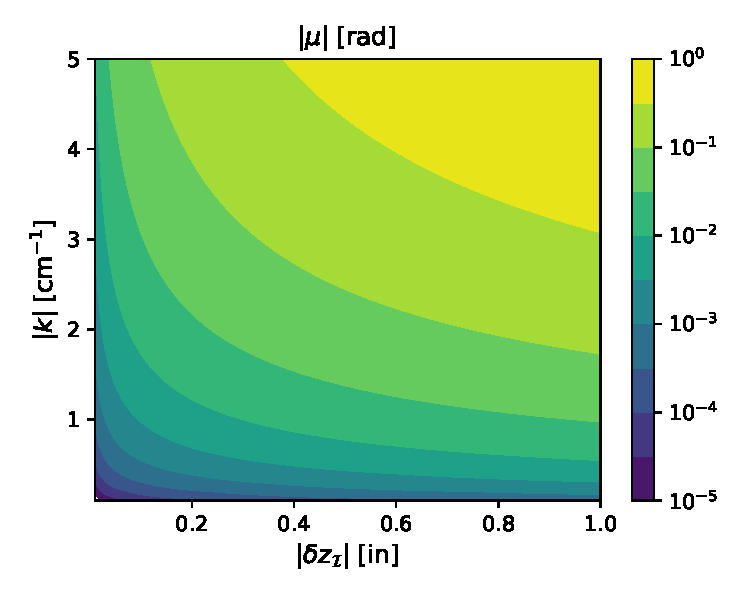
\includegraphics[width = 0.75 \textwidth]{%
    Chapters/Implementation/figs/wavenumber_dependent_phase_shift.pdf}
  \caption[Wavenumber-dependent phase shift from ``out-of-focus'' scattered beams]{%
    The wavenumber-dependent phase shift $\mu$ that occurs when
    the upscattered and downscattered $\SI{10.6}{\micro\meter}$ beams
    interfere a distance $\delta z_{\image}$ away from the image plane
    of an $M = 0.08$ imaging system; $|\mu| \ll 1$ is desirable.
  }
\label{fig:Implementation:wavenumber_dependent_phase_shift}
\end{figure}

Axial profiles of the unscattered beam and a scattered beam
in the design-point imaging system are shown in
Fig.~\ref{fig:Implementation:axial_beam_profiles}.
Because scattering from density fluctuations with larger wavenumbers
produces larger transverse deviations from the optical axis,
the scattered beam plotted in
Fig.~\ref{fig:Implementation:axial_beam_profiles}
corresponds to a $k = \SI{5}{\per\centi\meter}$ fluctuation, which
is the maximum measurable wavenumber
(\ref{eq:Implementation:kfsv_interferometer_design})
of the interferometer.
Note that the diameter of each focusing optic is accurately depicted
(if an optic touches the horizontal axes,
the optical diameter exceeds the plotted dimensions) and
that the aperture diffraction criterion
(\ref{eq:DesignConsiderations:summary:aperture_radius_for_minimal_diffraction})
is met for both the scattered and unscattered beams at each focusing optic.
For simplicity, planar mirrors are not depicted, but
they similarly satisfy the aperture diffraction criterion.
The probe radiation is combined with the reference beam and
interfered on a detector located at the second image plane,
approximately $395"$ downstream of the tokamak midplane.

\begin{figure}
  \centering
  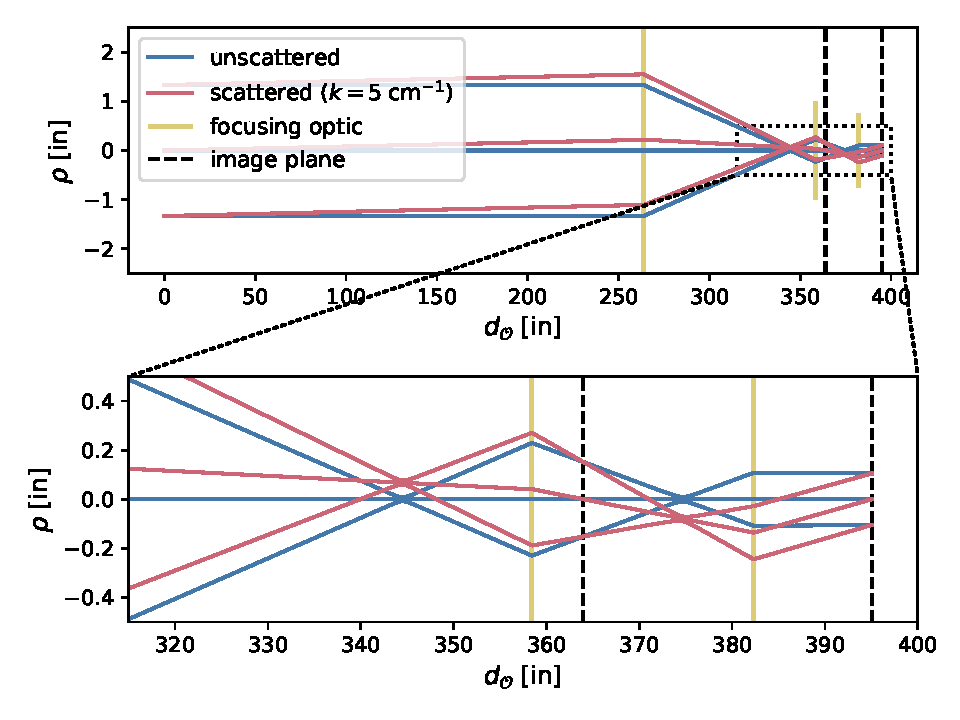
\includegraphics[width = \textwidth]{%
    Chapters/Implementation/figs/axial_beam_profiles.pdf}
  \caption[Axial beam profiles in interferometer probe arm]{%
    Axial beam profiles in interferometer probe arm
    as a function of distance $d_{\object}$ from
    the tokamak midplane (i.e.\ the object plane).
    For a given beam, the central ray corresponds to
    the symmetry axis of the beam, while
    the other two rays correspond to the 1/e $E$ radius of the beam.
    The interferometer detector sits at the second image plane,
    approximately $395"$ downstream of the tokamak midplane.
  }
\label{fig:Implementation:axial_beam_profiles}
\end{figure}


\section{Distribution of optical power}
\label{sec:Implementation:PowerDistribution}
Having identified a suitable heterodyne-interferometer optical layout in
Section~\ref{sec:Implementation:OpticalLayout},
the finite power of the $\SI{10.6}{\micro\meter}$ laser
must be distributed between the PCI and interferometer systems.
Section~\ref{sec:Implementation:PowerDistribution:gaussian_beam_intensity_and_power}
reviews the experimentally relevant relations between a Gaussian beam's
global properties (e.g.\ total beam power) and
local properties (e.g.\ peak, on-axis intensity).
Sections~\ref{sec:Implementation:PowerDistribution:pci_beam} through
\ref{sec:Implementation:PowerDistribution:interferometer_reference_beam}
develop approximate expressions for the total power
in the beam(s) at each detector location;
significantly, two design parameters, $\eta_R$ and $\eta_P$,
control the power distribution in the combined PCI-interferometer.
Finally, Section~\ref{sec:Implementation:PowerDistribution:constraints}
identifies a suitable operational point in $(\eta_R, \eta_P)$-space.


\subsection{Gaussian-beam intensity \& power}
\label{sec:Implementation:PowerDistribution:gaussian_beam_intensity_and_power}
The Gaussian-beam electric field
(\ref{eq:InterferometricMethods:Gaussian_beam})
produces the optical intensity (averaged over an optical cycle)
\begin{equation}
  I(\rho, z)
  =
  \frac{c \varepsilon_0}{2} |E_G(\vect{r})|^2
  =
  I(0, z) \exp\left[ \frac{-2 \rho^2}{w(z)^2} \right],
\end{equation}
where
\begin{equation}
  I(0, z)
  =
  \frac{c \varepsilon_0}{2}
  \left[ \frac{E_0 w_0}{w(z)} \right]^2
\end{equation}
is the peak, on-axis intensity of the Gaussian beam
at axial distance $z$ from the beam waist.
The optical power within $\rho_0$ of the symmetry axis is
\begin{equation}
  P(\rho \leq \rho_0)
  =
  \mathcal{P}
  \left\{ 1 - \exp\left[ \frac{-2 \rho_0^2}{w(z)^2} \right] \right\},
  \label{eq:Implementation:Gaussian_beam_power_circular_aperture}
\end{equation}
where
\begin{equation}
  \mathcal{P}
  =
  \frac{\pi [w(z)]^2}{2} \cdot I(0, z)
  \label{eq:Implementation:Gaussian_beam_total_power}
\end{equation}
is the \emph{total} optical power in the beam.
Similarly, the optical power within a square
of side length $s$ and centered on the optical axis is
\begin{equation}
  P
  =
  \mathcal{P} \left[ \erf\left( \frac{s}{\sqrt{2} w(z)} \right) \right]^2,
  \label{eq:Implementation:Gaussian_beam_power_square_aperture}
\end{equation}
where $\mathcal{P}$ is again the total optical power
(\ref{eq:Implementation:Gaussian_beam_total_power})
in the beam and
\begin{equation}
  \erf(z) = \frac{2}{\sqrt{\pi}} \int_0^z e^{-t^2} dt
  \label{eq:Implementation:error_function}
\end{equation}
is the error function.


\subsection{PCI beam}
\label{sec:Implementation:PowerDistribution:pci_beam}
Prior to the heterodyne-interferometer upgrade,
the total beam power at the PCI detector was
$\mathcal{P}_{\text{pci},0} \sim \SI{300}{\milli\watt}$.
The placement of the AOM in the expansion optics
produces a static $\sim 10\%$ optical insertion loss, and
driving the AOM with RF power deflects an additional fraction $\eta_R$
of the beam power to the reference arm of the interferometer.
Further, upstream of the phase plate,
a fraction $\eta_P$ of the beam power is diverted
to the probe arm of the interferometer.
Thus, after the upgrade, the total beam power at the PCI detector is
\begin{equation}
  \mathcal{P}_{\text{pci}}
  =
  0.9
  (1 - \eta_R)
  (1 - \eta_P)
  \mathcal{P}_{\text{pci},0}.
\end{equation}
To prevent substantial performance degradation of the PCI, the criterion
$\mathcal{P}_{\text{pci}} / \mathcal{P}_{\text{pci},0} \gtrsim 2 / 3$
is enforced.


\subsection{Interferometer probe beam}
\label{sec:Implementation:PowerDistribution:interferometer_probe_beam}
Upstream of the phase plate,
a fraction $\eta_P$ of the beam power is diverted
to the probe arm of the interferometer.
Recall that the phase-plate groove is uncoated ZnSe, which
reflects only $17\%$ of the unscattered probe beam.
Additionally, $50\%$ of the beam power is lost at the beam combiner
that combines the probe beam and the reference beam.
Thus, the total probe-beam power $\mathcal{P}_P$
at the heterodyne-interferometer detector
is given through power conservation as
\begin{equation}
  \mathcal{P}_{\text{pci}}
  +
  \left( \frac{0.17}{0.5} \right) \mathcal{P}_P
  =
  \mathcal{P}_{\text{pci},0}.
\end{equation}
(Of course, some of the beam power is also diverted
to the feedback system's quadrant detector, but
the power in this feedback beam was negligibly altered by the upgrade).
Using the probe-beam optical layout discussed in
Section~\ref{sec:Implementation:OpticalLayout:probe_beam},
the 1/e $E$ radius of the probe beam
at the heterodyne-interferometer detector is
\begin{equation}
  w_P = \SI{2.7}{\milli\meter}.
  \label{eq:Implementation:probe_beam_radius_at_detector}
\end{equation}


\subsection{Interferometer reference beam}
\label{sec:Implementation:PowerDistribution:interferometer_reference_beam}
The AOM produces a static $\sim 10\%$ optical insertion loss and
deflects a fraction $\eta_R$ of the remaining beam power
to the reference arm of the interferometer.
Additionally, $50\%$ of the beam power is lost at the beam combiner
that combines the probe beam and the reference beam.
Thus, the total reference-beam power $\mathcal{P}_R$
at the heterodyne-interferometer detector is
\begin{equation}
  \mathcal{P}_R
  =
  \left( \frac{0.9}{2} \right) \eta_R \mathcal{P}_S,
\end{equation}
where $\mathcal{P}_S \approx \SI{14}{\watt}$
is the total beam power at the laser source.
Using the reference-beam optical layout discussed in
Section~\ref{sec:Implementation:OpticalLayout:reference_beam_generation},
the 1/e $E$ radius of the probe beam
at the heterodyne-interferometer detector is
\begin{equation}
  w_R = \SI{4.3}{\milli\meter}.
  \label{eq:Implementation:reference_beam_radius_at_detector}
\end{equation}


\subsection{Constraining the distribution of optical power}
\label{sec:Implementation:PowerDistribution:constraints}
Suitably distributing the optical power in the combined PCI-interferometer
is an exercise in constrained optimization.
The objective function is the optical power
in the heterodyne-interference signal, while the constraints are
the operational limits of the interferometer detector and
the minimum required power in the PCI beam
($\mathcal{P}_{\text{pci}} / \mathcal{P}_{\text{pci},0} \gtrsim 2 / 3$).
Because the PCI constraint is somewhat ``soft'',
a graphical exploration of the design space is appropriate;
such a graphical exploration is shown in
Fig.~\ref{fig:Implementation:power_distribution}.
The \emph{top-left} panel of
Fig.~\ref{fig:Implementation:power_distribution}
displays the AC-to-DC multiplicative factor
$2 I_{\text{AC}} / (I_{\text{DC}} + I_{\text{AC}})$
from the heterodyne-interferometer transfer function
(\ref{eq:DesignConsiderations:summary:heterodyne_interferometer_wavenumber_transfer_function}).
The AC-to-DC multiplicative factor attains a maximum value of unity when
the AC and DC intensities of the heterodyne interference signal are equal
(i.e.\ when $I_{\text{AC}} = I_{\text{DC}}$).
Clearly, the AC-to-DC multiplicative factor
is a strong function of $\eta_R$, and
the design point achieves a reasonable balance
between the AC and DC components of the heterodyne signal.
A large value of $2 I_{\text{AC}} / (I_{\text{DC}} + I_{\text{AC}})$ alone
does \emph{not} guarantee optimal performance;
the normalizing peak intensity $I_{\text{DC}} + I_{\text{AC}}$
should also be maximized.
The \emph{top-right} panel of
Fig.~\ref{fig:Implementation:power_distribution}
displays this peak intensity.
The photovoltaic HgCdTe detectors that are often employed
for $\SI{10.6}{\micro\meter}$ heterodyne interferometry typically have
a saturation intensity
$I_{\text{sat}} = \SI{100}{\milli\watt\per\square\milli\meter}$
and a damage intensity
$I_{\text{dam}} = \SI{1}{\watt\per\square\milli\meter}$.
Note that $I_{\text{DC}} + I_{\text{AC}}$
is a strong function of $\eta_R$
and that $I_{\text{DC}} + I_{\text{AC}} \sim I_{\text{sat}}$
at the design point.
Depending on the saturation physics of the detector,
operating above $I_{\text{sat}}$ (but below $I_{\text{dam}}$)
may improve the system performance, as quantified by the
$V_1 / V_1(I_{\text{max}} = I_{\text{sat}})$ multiplicative factor
in the heterodyne-interferometer transfer function
(\ref{eq:DesignConsiderations:summary:heterodyne_interferometer_wavenumber_transfer_function}).
However, as the \emph{bottom-left} panel of
Fig.~\ref{fig:Implementation:power_distribution} shows,
the constraint
$\mathcal{P}_{\text{pci}}
\gtrsim
(2 / 3) \mathcal{P}_{\text{pci},0}
\sim \SI{200}{\milli\watt}$
prevents operating the heterodyne interferometer
with intensities above $I_{\text{sat}}$.
This inability to operate above $I_{\text{sat}}$ can be compensated
by actively cooling the detector to improve its sensitivity.
\graffito{\textcolor{red}{Describe elsewhere?}}
The interferometer described in this thesis
uses two-stage thermoelectric cooling
to cool the detector to $T \sim \SI{230}{\kelvin}$,
boosting the specific detectivity $D^*$ by an order of magnitude;
the cooling capacity is limited to
$Q_{\text{heat}} \lesssim \SI{75}{\milli\watt}$.
Because the total power in the probe beam and the reference beam
greatly exceeds this cooling capacity,
a circular aperture of radius $a = \SI{0.75}{\milli\meter}$
is positioned immediately upstream of the detector;
the power of a Gaussian beam passing through such an aperture is given by
(\ref{eq:Implementation:Gaussian_beam_power_circular_aperture})
such that the heat that must be dissipated reduces to
\begin{equation}
  Q_{\text{heat}}
  =
  \mathcal{P}_P
  \left[ 1 - \exp\left( \frac{-2 a^2}{w_P^2} \right) \right]
  +
  \mathcal{P}_R
  \left[ 1 - \exp\left( \frac{-2 a^2}{w_R^2} \right) \right].
\end{equation}
The \emph{bottom-right} panel of
Fig.~\ref{fig:Implementation:power_distribution}
displays $Q_{\text{heat}}$.
Now, in practice, $\eta_P$ is fixed by the reflectivity
of the ZnSe splitter located upstream of the phase plate
(with $25\%$ reflectivity being a common, off-the-shelf value);
then, during an alignment, $\eta_R$ is increased slowly
until the cooling capacity of the detector is reached.

\begin{figure}
  \centering
  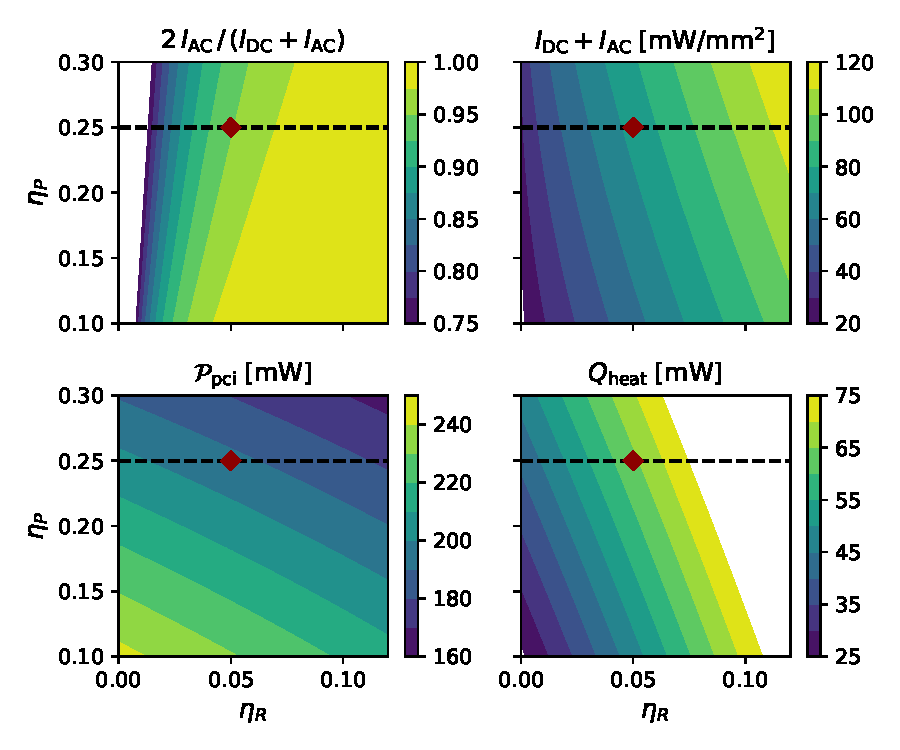
\includegraphics[width = \textwidth]{%
    Chapters/Implementation/figs/power_distribution.pdf}
  \caption[Constraints on the distribution of optical power]{%
    Constraints on the distribution of optical power
    in the combined PCI-interferometer.
    The AOM deflection efficiency,
    which governs the fraction $\eta_R$
    of beam power diverted to the interferometer reference arm,
    is displayed along the $x$-axis.
    The fraction $\eta_P$ of probe-beam power
    (immediately upstream of the phase plate)
    diverted to the interferometer probe arm
    is displayed along the $y$-axis.
    All intensities correspond to peak, on-axis values.
    The design point is marked with a burgundy diamond;
    note that $\eta_P = 0.25$ is fixed for the installed splitter, but
    varying the AOM RF power readily changes $\eta_R$,
    allowing easy movement along the horizontal dashed line.
    See text for discussion.
  }
\label{fig:Implementation:power_distribution}
\end{figure}


\section{Dedicated heterodyne-interferometer hardware}
\label{sec:Implementation:Hardware}
\graffito{\textcolor{red}{laser parameters?}}
Utilizing a shared in-vessel probe beam implies that
the PCI and the heterodyne interferometer share several components,
including the CO$_2$ laser,
the beam expansion optics, and
the beam-delivery and beam-collection optics.
\graffito{\textcolor{red}{digitizer parameters?}}
The two systems also share a digitizer.
Numerous other components, however,
are exclusively dedicated to the operation
of the heterodyne interferometer.
Some of these components have been discussed in previous sections
(i.e.\ the reference-beam optics
in Section~\ref{sec:Implementation:OpticalLayout:reference_beam_generation}
and the probe-beam imaging optics
in Section~\ref{sec:Implementation:OpticalLayout:probe_beam}).
This section details the remainder
of the heterodyne interferometer's dedicated hardware.


\subsection{Oven-controlled crystal oscillator (OCXO)}
\label{sec:Implementation:Hardware:OCXO}
\graffito{\textcolor{red}{cite AoE?}}
Placing a crystal oscillator (XO) in a constant-temperature thermal bath
substantially improves the XO stability,
dramatically reducing the XO phase noise.
For technical reasons,
ovens operated tens of degrees above the ambient temperature
provide the most robust constant-temperature thermal baths.
Such an oven-controlled crystal oscillator (OCXO)
can achieve stabilities that are \textcolor{red}{orders-of-magnitude larger}
than a comparable XO.

The local oscillator (LO) of the heterodyne interferometer
is derived from an OCXO.
The OCXO was procured from Wenzel Associates, Inc. (Austin, TX USA)
and is enclosed in their Sprinter packaging.
The OCXO has a $5$-minute warm-up time,
during which it draws a maximum power of $\SI{5}{\watt}$;
after warming up, it draws $\SI{2.2}{\watt}$.
The OCXO output is a $13 \; \text{dBm}$ sinusoidal signal
at a frequency of $\SI{30}{\mega\hertz}$
(i.e.\ in the notation of
Chapters~\ref{ch:InterferometricMethods} and \ref{ch:DesignConsiderations},
$\Delta \omega_0 = 2 \pi \cdot \SI{30}{\mega\hertz}$).
The OCXO phase noise is
\begin{equation}
    \mathcal{L}_{\Delta \omega_0}(f)
    =
    -165 \; \text{dBc},
    \qquad
    f \geq \SI{10}{\kilo\hertz}.
  \label{eq:Implementation:OCXO_phase_noise}
\end{equation}
The conversion between $\text{dBc}$ and
$\SI{}{\radian\squared\per\hertz}$ is discussed
in Appendix~\ref{app:OscillatorPhaseNoise}.

A custom, rack-mounted module was built to house the OCXO.
The module housing protects the OCXO from rough handling and
encloses additional electronics that facilitate
the OCXO integration into the rest of the heterodyne-interferometer system.
The OCXO module is installed in the PCI rack
located in the \diiid\space annex.
A schematic of this module is shown in
Fig.~\ref{fig:Implementation:OCXO_module}.
A $\SI{15}{\volt}$ linear-regulated power supply
($15EB40$, Acopian Technical Co.; Easton, PA USA)
powers the OCXO, while
a $\SI{5}{\volt}$ linear-regulated power supply ($5EB50$, Acopian)
powers the thermal-regulation and RF-modulation electronics.
Linear-regulated power supplies are less noisy than
either switching-mode or unregulated power supplies, so
it was deemed essential to power the OCXO
with a linear-regulated power supply.
To prevent overheating the AOM
(e.g.\ due to a water-cooling failure),
a normally closed, creep-action thermostat
(Pepi Model N, Portage Electric Products, Inc; North Canton, OH USA)
monitors the AOM temperature;
if the AOM temperature exceeds $\SI{30}{\celsius}$,
the thermostat opens.
Now, assuming the AOM temperature is less than $\SI{30}{\celsius}$,
connecting the thermostat of the AOM
to the thermal interlock of the OCXO module
produces a current that closes the normally open, non-latching relay
that sits between the $\SI{15}{\volt}$ linear-regulated power supply
and the OCXO, powering on the OCXO.
The OCXO signal is evenly split via
a Mini-Circuits (Brooklyn, NY USA) {ZFSC-$2$-$6$B} RF splitter
to produce two LO signals;
one of the LO signals is routed to the AOM RF driver
(described in Section~\ref{sec:Implementation:Hardware:RF_driver})
located in the \diiid\space pit, and
the other LO signal is routed to the interferometer demodulation electronics
(described in
Section~\ref{sec:Implementation:Hardware:demodulation_electronics})
located in the PCI rack of the \diiid\space annex.
A Mini-Circuits {FTB-$1$-$1$} balun transformer
breaks the ground loop between the OCXO module and the AOM RF driver.
A Mini-Circuits {ZSDR-$230$+} RF switch also enables amplitude modulation
of the LO signal that is routed to the AOM RF driver;
this capability is only used during system alignment, as described in
Section~\ref{sec:Implementation:Alignment}.
Finally, a switch at the rear of the module
allows one to easily toggle the module grounding between
the electrical mains (i.e.\ for bench testing) and
the PCI rack (i.e.\ for operations).

\begin{figure}
  \centering
  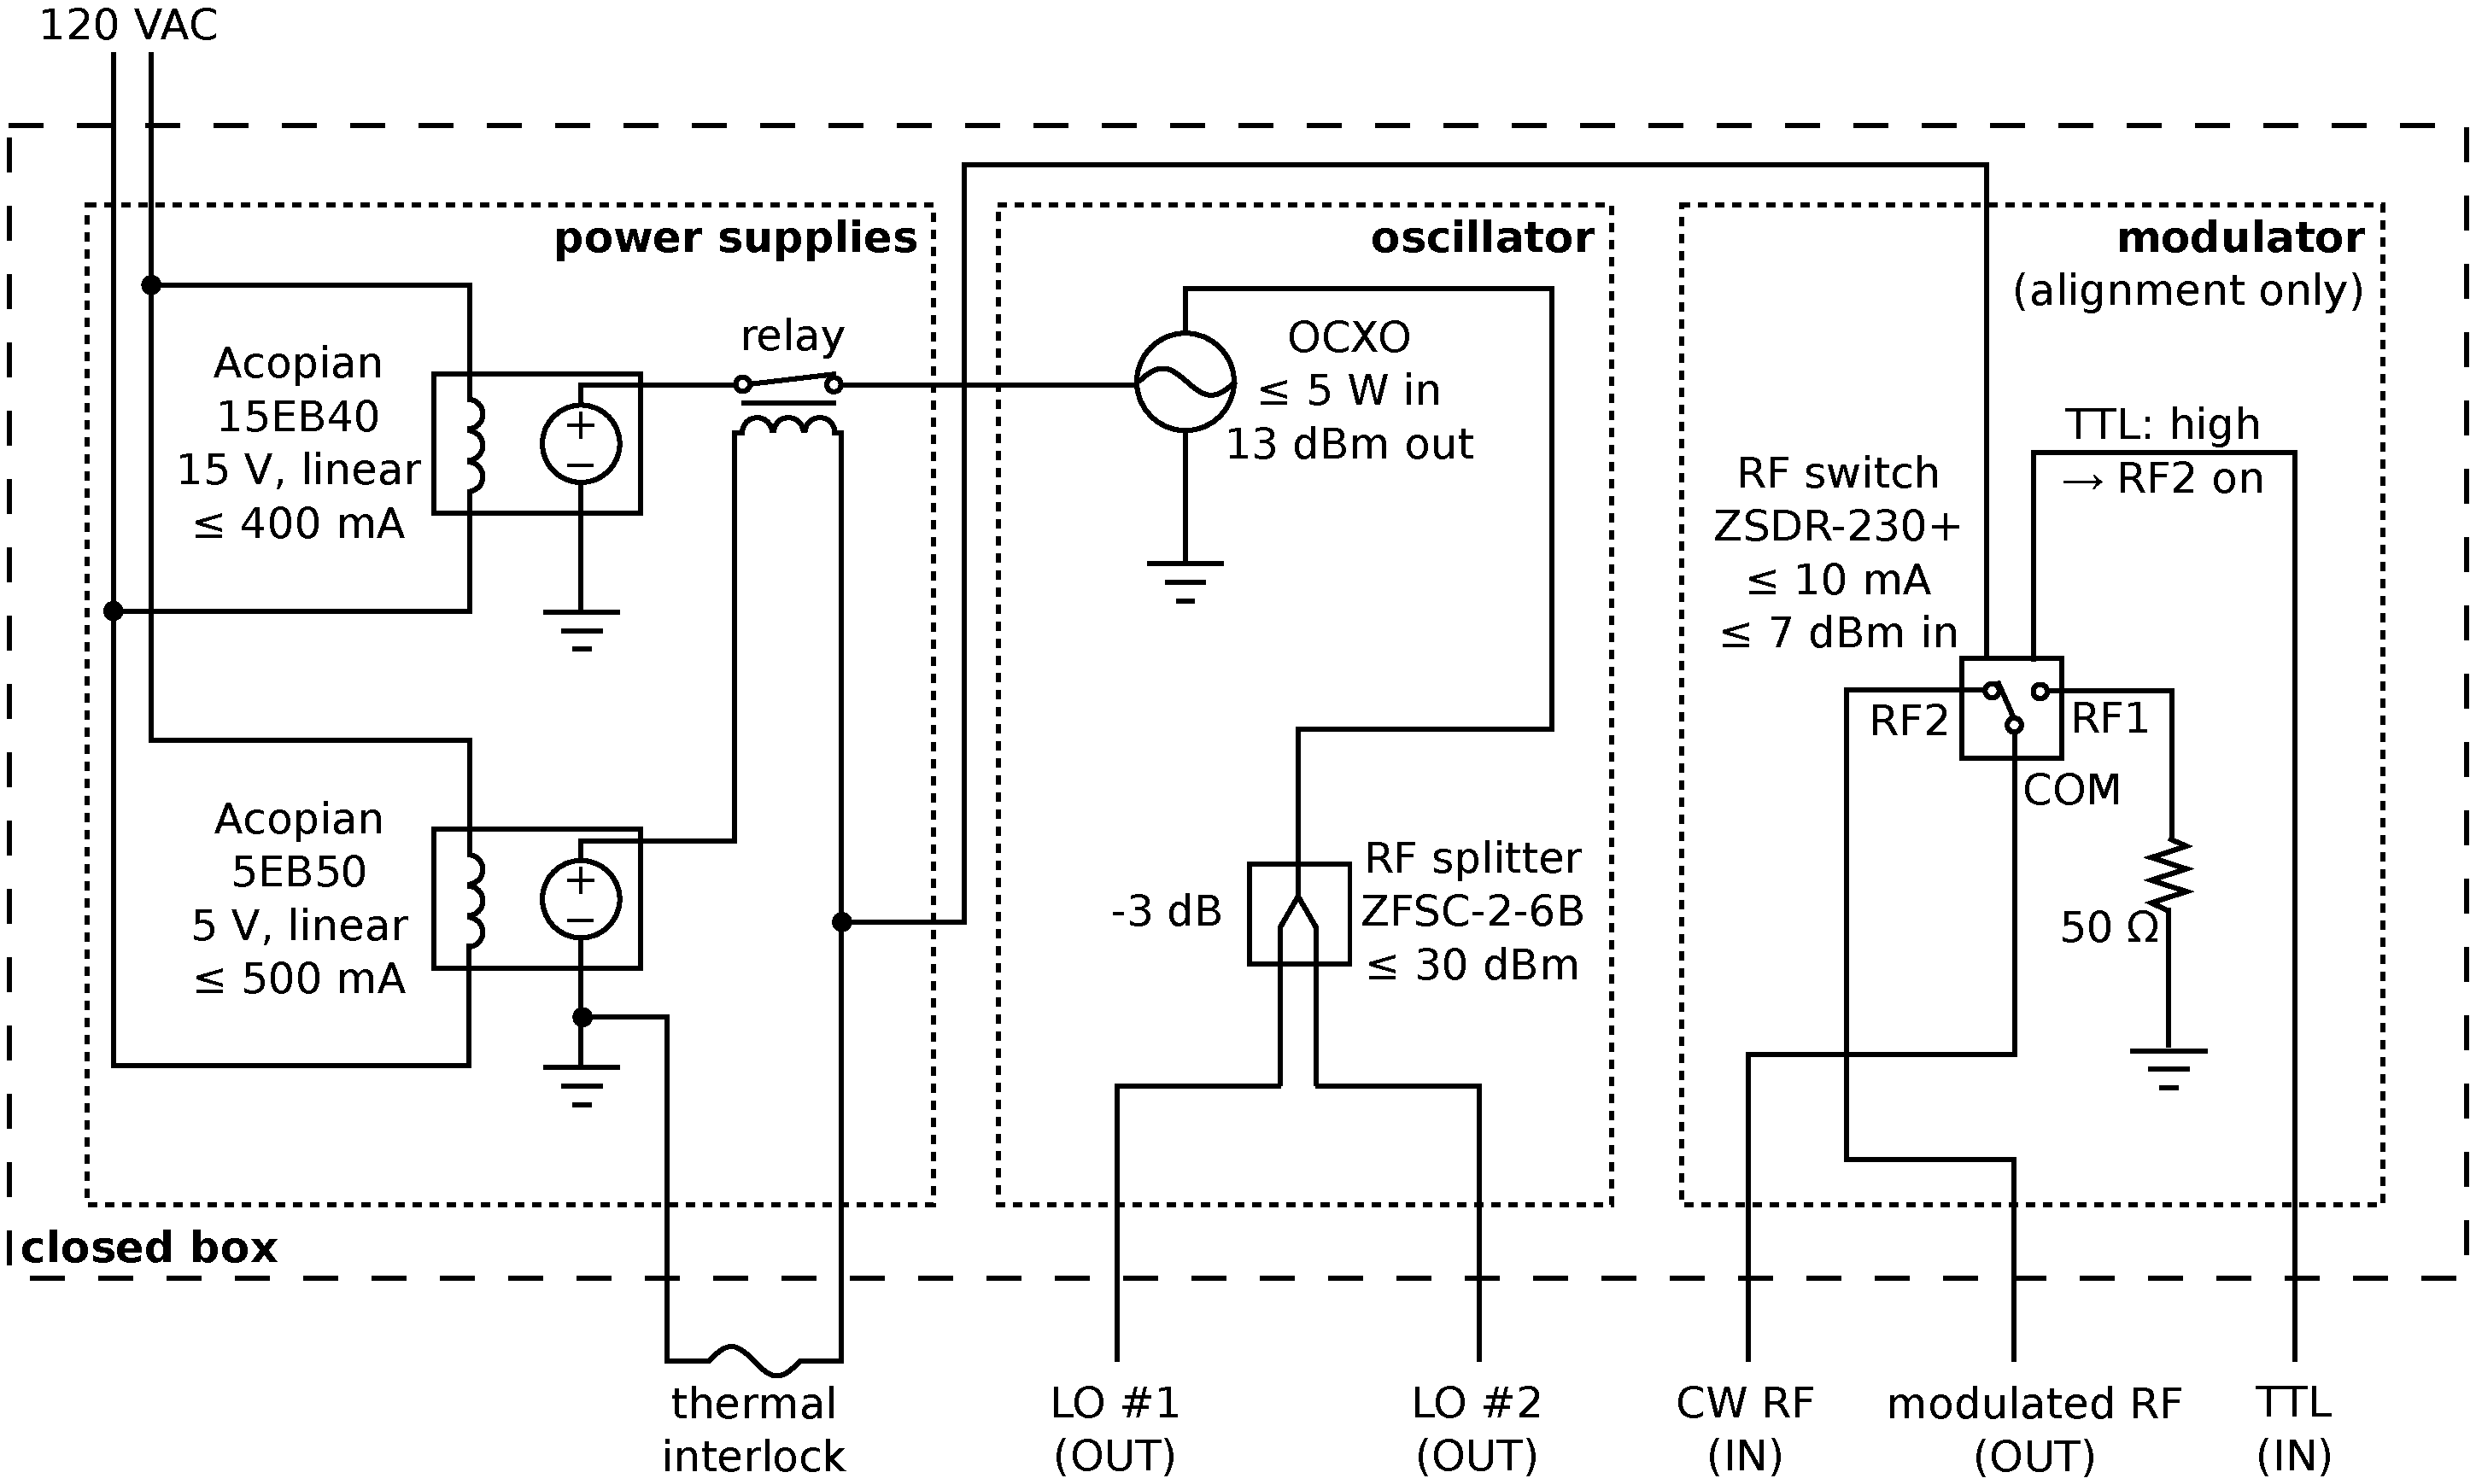
\includegraphics[width = \textwidth]{%
    Chapters/Implementation/figs/OCXO_module.pdf}
  \caption[Schematic for OCXO rack-mounted module]{%
    Schematic for OCXO rack-mounted module. See text for details.}
  \label{fig:Implementation:OCXO_module}
\end{figure}


\subsection{AOM RF driver}
\label{sec:Implementation:Hardware:RF_driver}
The LO signal must be amplified to several watts in order to drive the AOM.
An ENI (Rochester, NY USA) $3100L$ performs this amplification.
(Note that ENI no longer exists but that
the closely related E\&I currently manufactures comparable amplifiers).
The $3100L$ provides broadband power amplification between
$\SI{250}{\kilo\hertz}$ to $\SI{105}{\mega\hertz}$.
The $3100L$ has $\SI{50}{\decibel}$ gain
and a rated power output above $\SI{100}{\watt}$
(as the AOM is typically driven at $\sim \SI{1}{\watt}$,
the $3100L$ greatly exceeds the drive requirements;
note that the $3100L$ is on long-term loan from the $\diiid$ RF group,
though, and they had no suitable, lower-power amplifiers).
The harmonic distortion of the $3100L$ is $\leq -25 \; \text{dBc}$, and
its noise figure is $\leq \SI{10}{\decibel}$.
\graffito{\textcolor{red}{cite self-demodulation methodology}}
Self-demodulation tests conducted with and without the $3100L$
demonstrate that the $3100L$ does \emph{not} add appreciable
noise into the interferometer measurements.
The $3100L$ draws $\SI{1.1}{\kilo\watt}$ of $120$ VAC wall power;
a $2.4 \; \text{kVA}$ Topaz isolation transformer
isolates the $3100L$ from high-frequency wall-power noise.
At a hefty $70 \; \text{lbs}$,
the $3100L$ is mounted in the PCI rack
adjacent to the PCI optical table in the \diiid\space pit;
the Topaz isolation transformer is mounted
to the pit wall behind the PCI rack.
\graffito{\textcolor{red}{coax line length?}}
The AOM drive level is adjusted by appropriately attenuating
the LO signal just upstream of the $3100L$ input;
this ``just-in-time'' attenuation minimizes the effect of electrical pickup
during the signal transit from the annex to the pit
(relative to e.g.\ attenuating the signal in the annex
and then sending the signal to the pit).


\subsection{Detector}
\label{sec:Implementation:Hardware:detector}
\graffito{\textcolor{red}{cite VIGO}}
Detection of $\SI{10.6}{\micro\meter}$ light
is typically effected with Mercury Cadmium Telluride (HgCdTe),
an alloy of HgTe and CdTe.
The ratio of HgTe to CdTe is tuned to provide
optimal detection at the device's intended operational temperature.
Cooling the HgCdTe typically
increases the cut-off wavelength,
increases optical responsivity, and
decreases device noise,
but often at the expense of device speed.
Device noise and speed also depend on whether
the HgCdTe detector is photovoltaic (PV) or photoconductive (PC);
in particular, PC detectors exhibit $1 / f$ noise and
are often slower than their PV counterparts.

Resolving the temporal dynamics
of the heterodyne interferometer's $\SI{30}{\mega\hertz}$ signal
requires a sufficiently fast detector.
This immediately precludes the use of a liquid-nitrogen cooled detector,
as is used for the PCI.
Room-temperature HgCdTe detectors are sufficiently fast but
also exhibit relatively low sensitivity.
Modest thermoelectric (TE) cooling, however,
can engender some of the positive aspects of cooling while
maintaining sufficient time resolution.

The $\SI{30}{\mega\hertz}$ heterodyne-interference signal is measured with
a {PVM-$2$TE-$10.6$} detector element mounted on a MIPACv$2$ detection module,
both procured from VIGO System S.A. (Ozarow Mazowiecki, Poland).
The multiple-junction PV element provides superior speed
($\SI{3}{\decibel}$ high-frequency cutoff $\sim \SI{50}{\mega\hertz}$) and
sensitivity ($D^* \sim \SI{1.9e8}{\centi\meter \sqrt\hertz \per\watt}$)
relative to a PC element or a single-junction PV element.
The element is square with side length $s_x = \SI{1}{\milli\meter}$,
in accordance with (\ref{eq:Implementation:detector_size}).
The element has linear saturation intensity
$I_{\text{sat}} = \SI{100}{\milli\watt\per\milli\meter\squared}$ and
damage intensity
$I_{\text{dam}} = \SI{1}{\watt\per\milli\meter\squared}$.
The element and TE cooler are enclosed
in TO-$8$ packaging with a BaF$_2$ window;
care should be taken not to scratch the soft BaF$_2$ window or
to subject the system to mechanical shocks, which
may damage the TE cooler.
The TE cooler is capable of maintaining the detector element
at a constant $\SI{235}{\kelvin}$ temperature
for incident DC optical fluxes $\lesssim \SI{75}{\milli\watt}$.
The MIPACv$2$ detection module houses additional TE-cooling components
as well as the detector preamplifier.
The preamplifier is AC-coupled with
a cut-on frequency of $\SI{1}{\kilo\hertz}$ and
a cut-off frequency of $\SI{50}{\mega\hertz}$, and
it is capable of producing a $\pm\SI{1}{\volt}$
output-voltage swing into a $\SI{50}{\ohm}$ load.
The MIPACv$2$ detection module is powered by
VIGO's STCC-$04$ controller.
The specific detectivity of the element and the detection module
taken as an integrated unit is
\begin{equation}
  D^* = \SI{5.35e7}{\centi\meter \sqrt\hertz \per\watt}.
  \label{eq:Implementation:Dstar}
\end{equation}
The detector module is pictured in
Fig.~\ref{fig:Implementation:detector}.

\begin{figure}
  \centering
  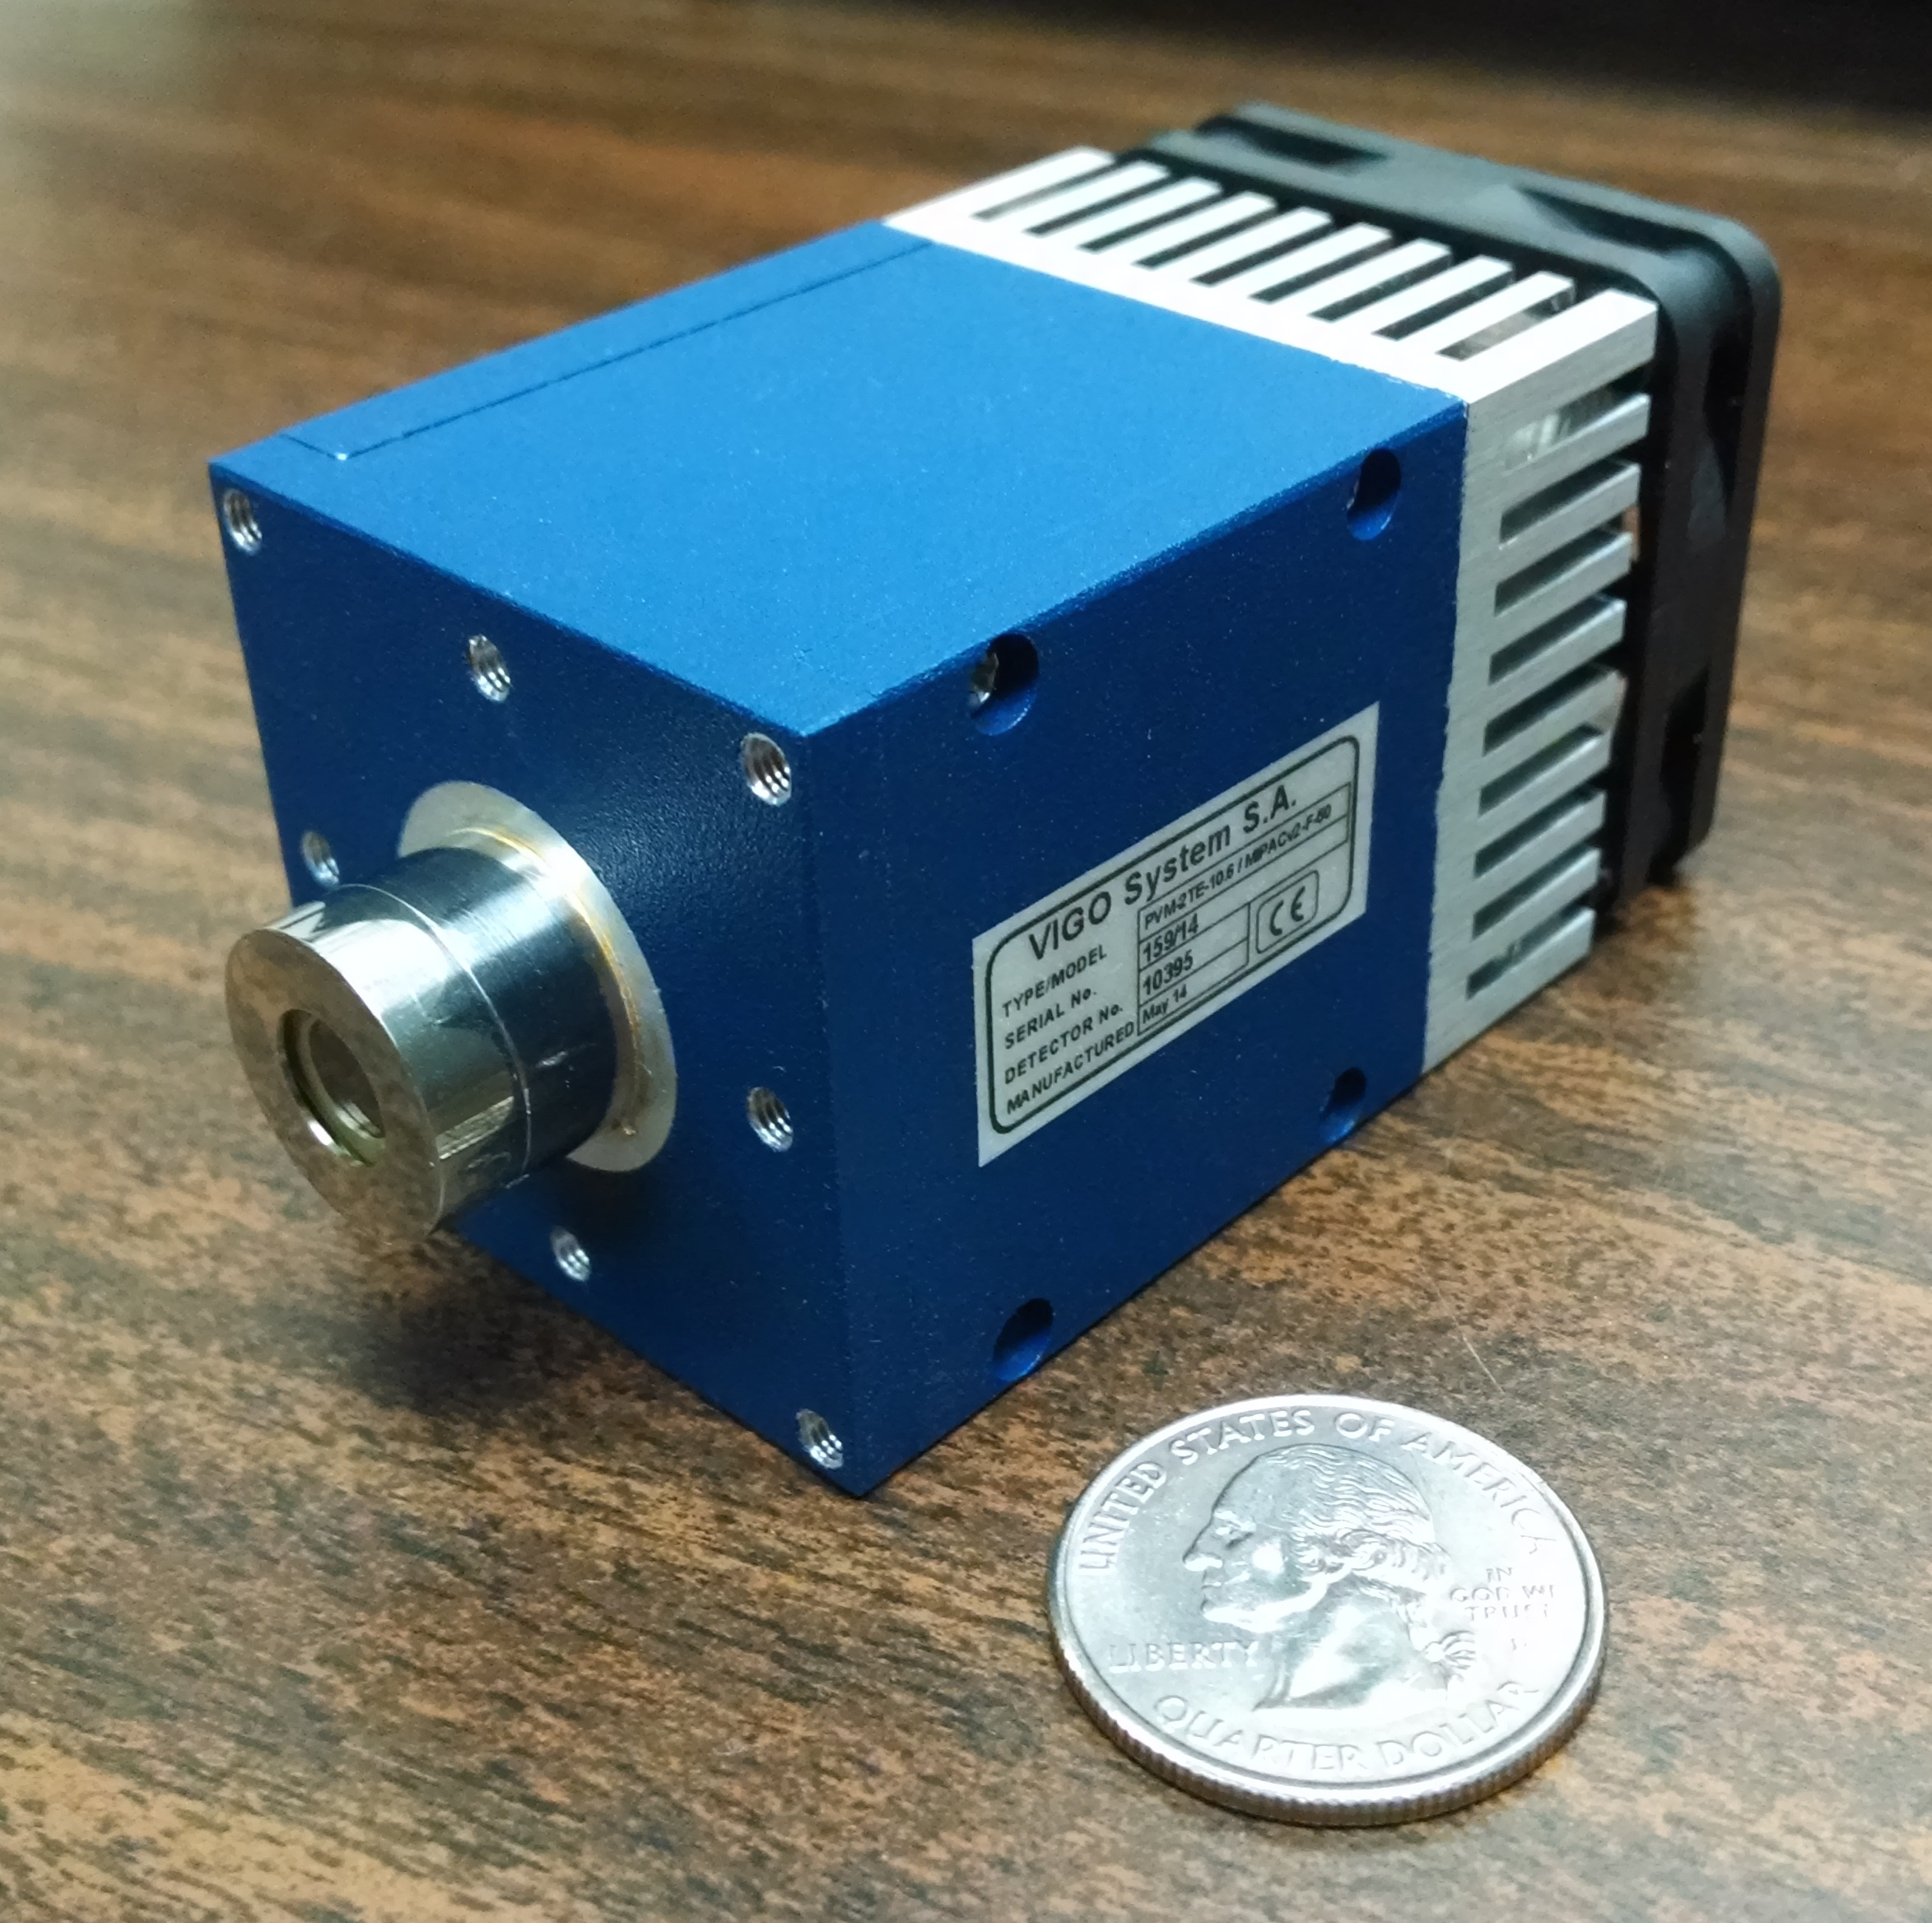
\includegraphics[width = 0.6 \textwidth]{%
    Chapters/Implementation/figs/detector.jpg}
  \caption[Detector module]{%
    The heterodyne interferometer's detector module.
    The detector element and thermoelectric (TE) cooler
    are enclosed within the TO-$8$ silver ``can'' at middle left.
    The blue housing encloses additional TE-cooling components and
    the detector preamplifier.
    A heat sink and small fan are located opposite of the detector face.
    The female SMA connector (for detector output) and
    the receptacle for a $9$-pin LEMO cable
    (for communication with the module controller)
    sit on the unpictured side of the detector module.
  }
\label{fig:Implementation:detector}
\end{figure}


\subsection{Coaxial cables to \diiid\space annex}
\label{sec:Implementation:Hardware:coax}
RG-$58$ coaxial cables transmit signals
between the interferometer components
located in the \diiid\space annex and the \diiid\space pit.
Initially installed for PCI signal transmission but
abandoned following an upgrade to fiber-optic links
\cite[Sec.~3.3.3]{dorris_phd},
these cables were reclaimed for the interferometer.
The $16$ cables sit bundled beneath the PCI optical table and
connect to channels $C27$ through $C42$
of panel $5B$ in the \diiid\space annex.
The single-transit propagation time of each cable
was measured to be $\SI{315}{\nano\second}$
by launching a square wave of modest frequency
(tens of $\SI{}{\kilo\hertz}$)
down the \emph{unterminated} cable and
halving the observed time delay between the forward and reflected waves.
As RG-$58$ has an index of refraction $\sim 3 / 2$,
this corresponds to a cable length of $\SI{63}{\meter}$.
DC signals are negligibly attenuated along this cable length, but
AC signals are subject to the skin effect
\cite[Sec.~H.1.4]{horowitz_and_hill};
the measured attenuation at $\SI{30}{\mega\hertz}$ is $\SI{5.9}{\decibel}$.
The DC signal between the AOM thermostat and
the thermal interlock of the OCXO module
travels along one of these coaxial cables.
A second coaxial cable transmits
one of the $\SI{30}{\mega\hertz}$ LO signals
from the OCXO module
to the AOM RF driver, and
a third coaxial cable transmits
the $\SI{30}{\mega\hertz}$ heterodyne-interference signal
from the interferometer detector
to the signal-conditioning RF amplifiers.


\subsection{Signal-conditioning RF amplifiers}
\label{sec:Implementation:Hardware:RF_amps}
Despite feedback stabilization of the beam coalignment
(discussed in
Sections~\ref{sec:Implementation:OpticalLayout:coalignment_with_feedback})
and \ref{sec:Implementation:OpticalLayout:probe_beam}),
vibration-induced misalignment can still substantially reduce
the amplitude of the heterodyne-interference signal,
dramatically degrading the signal-to-noise ratio of the interferometer.
These amplitude variations can be compensated
with an automatic gain-control (AGC) amplifier, which
monitors the amplitude of the input signal and
dynamically adjusts its gain
to maintain a constant-amplitude output signal.

An AGC amplifier was graciously provided \emph{pro bono}
by Palomar Scientific Instruments (San Marcos, CA USA).
The AGC operates over a frequency range from
$\SI{20}{\mega\hertz}$ to $\SI{100}{\mega\hertz}$.
The AGC produces a $-6 \; \text{dBm}$ output signal for
an input signal between $-24 \; \text{dBm}$ and $+6 \; \text{dBm}$;
the input damage limit is $20 \, \text{dBm}$.
The input and output impedances are both $\SI{50}{\ohm}$, and
the input and output ports are female SMA.
The AGC draws $\SI{160}{\milli\amp}$
from a DC power supply that can sit
anywhere between $\SI{7}{V}$ and $\SI{15}{V}$;
however, higher DC voltages produce significant heat dissipation, and
operation at the upper limit of $\SI{15}{V}$ should be avoided, if possible.
The AGC is shown in Fig.~\ref{fig:Implementation:AGC}.
If the heterodyne interference signal falls
below the lower limit of the AGC input range
(e.g. due to long-term drift of the system alignment),
a Mini-Circuits (Brooklyn, NY USA) {ZFL-$500$B} amplifier
is added immediately upstream of the AGC.

\begin{figure}
  \centering
  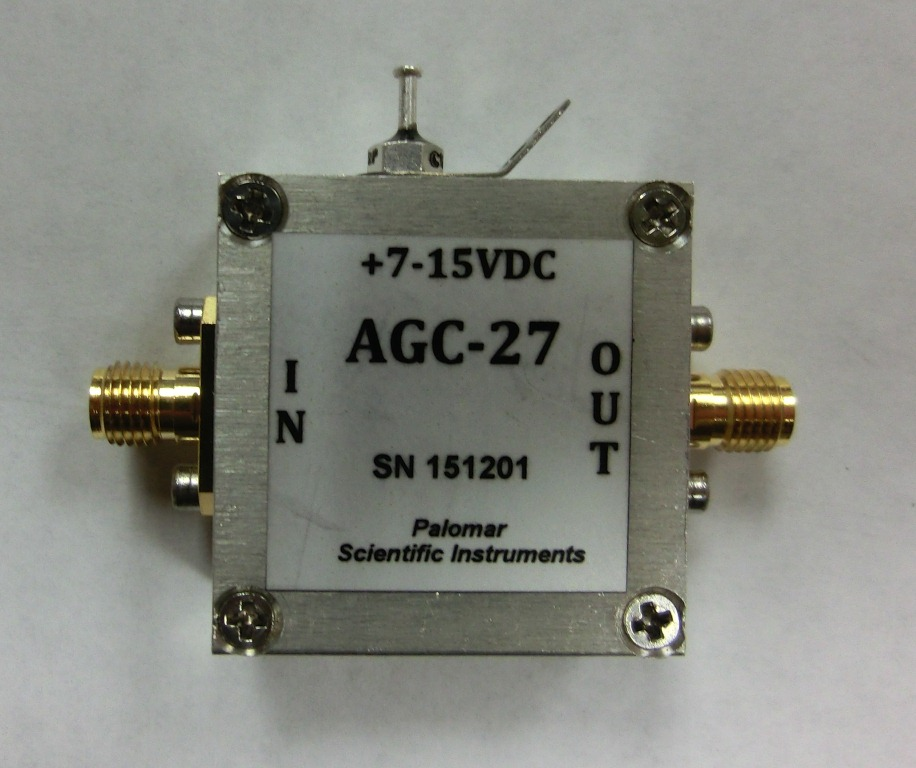
\includegraphics[width = 0.5 \textwidth]{%
    Chapters/Implementation/figs/AGC27.jpg}
  \caption[Automatic gain-control (AGC) amplifier]{%
    Automatic gain-control (AGC) amplifier.
  }
  \label{fig:Implementation:AGC}
\end{figure}

These signal-conditioning RF amplifiers
are located in the PCI rack of the \diiid\space annex.
A $\SI{12}{\volt}$ linear-regulated power supply
($12EB40$, Acopian Technical Co.; Easton, PA USA)
powers the amplifiers.
A Mini-Circuits {FTB-$1$-$1$} balun transformer
breaks the ground loop between
the interferometer detector and the signal-conditioning RF amplifiers.


\subsection{Demodulation electronics}
\label{sec:Implementation:Hardware:demodulation_electronics}
The theory of ideal and real-world demodulation is discussed in
Section~\ref{sec:DesignConsiderations:demodulation}, and
readers are encouraged to review that section
if context for the hardware described below is desired.
A schematic of the demodulation electronics is shown in
Fig.~\ref{fig:Implementation:demodulation_electronics}.

\begin{figure}
  \centering
  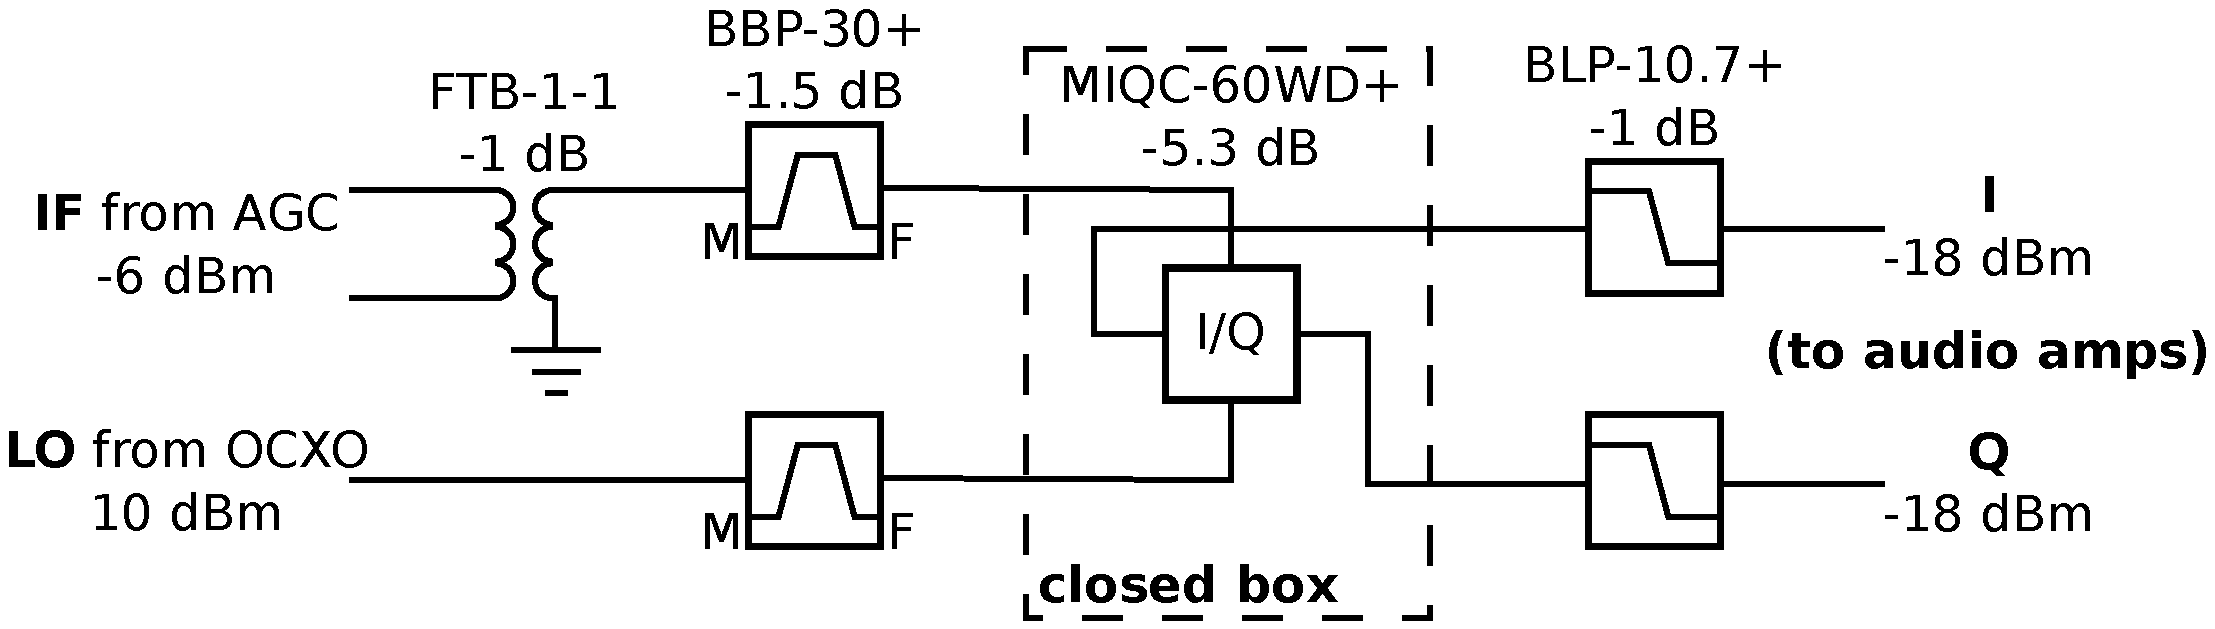
\includegraphics[width = \textwidth]{%
    Chapters/Implementation/figs/demodulation_electronics.pdf}
  \caption[Schematic for demodulation electronics]{%
    Schematic for demodulation electronics.
    Note that the polarity of the bandpass filters
    is explicitly noted as M (male) and F (female).
    The OCXO and the electronics downstream of the $I\&Q$ demodulator
    are all grounded to the PCI rack in the \diiid\space annex;
    the IF signal conditioning amplifiers
    are \emph{not} grounded to the rack,
    so a balun transformer breaks the ground loop.
    Measurements along any point in the circuit
    should be into $\SI{50}{\ohm}$.
  }
  \label{fig:Implementation:demodulation_electronics}
\end{figure}

Prior to demodulation, the LO and IF signals are each bandpass filtered
with a Mini-Circuits (Brooklyn, NY USA) {BBP-$30$+}.
The {BBP-$30$+} has $\leq \SI{1.5}{\decibel}$ insertion loss over
its $\SI{27}{\mega\hertz}$ to $\SI{33}{\mega\hertz}$ passband.
Bandpass filtering the $\SI{30}{\mega\hertz}$ IF
suppresses higher-order harmonics and out-of-band noise,
both of which would degrade the heterodyne interferometer's phase measurement.
Although Section~\ref{sec:DesignConsiderations:demodulation:nonideal_mixing}
discusses the potential benefits of demodulating against a square LO,
no such LO was available, so
the LO is instead bandpass filtered
to ensure that the IF is demodulated against a sinusoid.
The {BBP-$30$+} is \emph{directional}, so
care should be taken to install the filter
with the correct orientation.
Following the bandpass filter,
a Mini-Circuits {FTB-$1$-$1$} breaks the ground loop between
the IF signal-conditioning amplifiers and
the audio amplifiers.
The resulting $-8.5 \; \text{dBm}$ IF and $8.5 \; \text{dBm}$ LO
are now ready to be demodulated.

Demodulation is performed with a
Mini-Circuits {MIQC-$60$WD+}
analog $I\&Q$ demodulator.
The {MIQC-$60$WD+} can demodulate IF signals with frequencies between
$\SI{20}{\mega\hertz}$ and $\SI{60}{\mega\hertz}$, while
the bandwidth of the resulting $I$ and $Q$ signals
may span from DC up to $\SI{5}{\mega\hertz}$.
\graffito{\textcolor{red}{reference for ``deadbug''?}}
To minimize parasitic capacitances,
the {MIQC-$60$WD+} is soldered ``deadbug'' style
to a large grounding plane, and
every electrical connection is soldered
directly to its corresponding pin;
the demodulator, wiring, and grounding plane
are enclosed in a protective box with external BNC jacks.
The {MIQC-$60$WD+} conversion loss is $\SI{5.3}{\decibel}$.
The amplitude imbalance is $\leq \SI{0.6}{\decibel}$,
the phase imbalance $\leq \SI{5}{\degree}$, and
the DC offset is typically $\sim \SI{1}{\milli\volt}$.
The $3$\ts{rd}- and $5$\ts{th}-order harmonic suppressions
were measured to be $\SI{53}{\decibel}$ and $\SI{64}{\decibel}$, respectively.

The signals exiting the $I$ and $Q$ ports of the demodulator
must be low-pass filtered
to remove the $\SI{60}{\mega\hertz}$ ``sum'' components
that result from mixing the LO and IF.
Low-pass filtering is performed
with a pair of Mini-Circuits {BLP-$10.7$+} filters, which
have $\leq \SI{1}{\decibel}$ insertion loss
over their DC to $\SI{11}{\mega\hertz}$ passband.
The resulting $I$ and $Q$ signals are each
$-18 \; \text{dBm}$
(i.e.\ $\SI{28.2}{\milli\volt}$ RMS,
$\SI{80}{\milli\volt}$ peak-to-peak).


\subsection{Audio amplifiers}
\label{sec:Implementation:Hardware:audio_amps}
\graffito{\textcolor{red}{digitizer parameters?}}
The demodulated $I$ and $Q$ signals are $\SI{80}{\milli\volt}$ peak-to-peak,
while the digitizer dynamic range is $V_{\text{dyn}} = \SI{8}{\volt}$.
Thus, direct digitization of the $I$ and $Q$ signals
corresponds to a fractional use $\eta_{\text{dyn}} = 0.01$
of the digitizer's dynamic range.
When $\eta_{\text{dyn}} = 0.01$,
the autospectral density of the corresponding quantization noise
(\ref{eq:DesignConsiderations:summary:quantization_noise_autospectral_density})
is $10^4$ \emph{larger} than when $\eta_{\text{dyn}} = 1$;
the $\eta_{\text{dyn}} = 0.01$ quantization noise
is shown to be unacceptably large in \textcolor{red}{Section XXX}.
To minimize quantization noise, then, the $I$ and $Q$ signals
must be amplified to $\eta_{\text{dyn}} \approx 1$ prior to digitization.

\begin{figure}
  \centering
  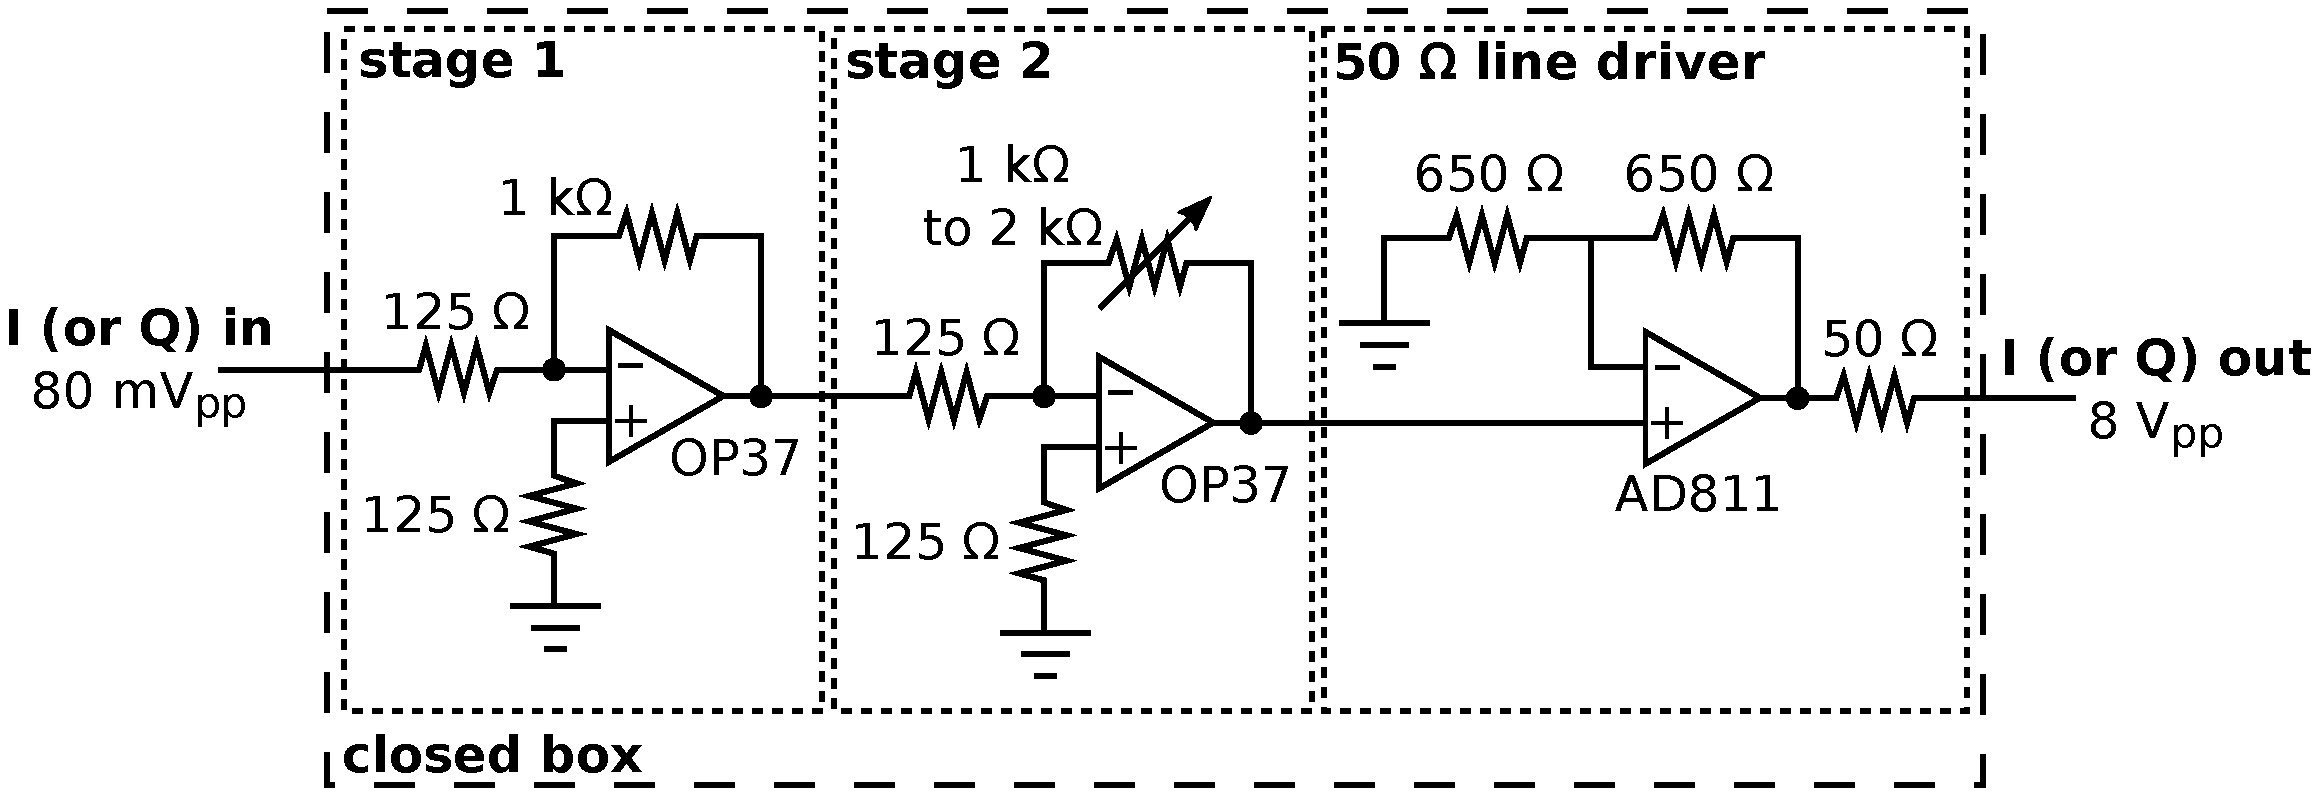
\includegraphics[width = \textwidth]{%
    Chapters/Implementation/figs/audio_amp_schematic.pdf}
  \caption[Audio-amplifier schematic]{%
    Audio-amplifier schematic.
    The amplifier consists of
    two high-gain, low-noise amplification stages
    followed by a $\SI{50}{\ohm}$ line driver,
    which is required to drive the digitizer's
    $\SI{50}{\ohm}$ input impedance.
  }
\label{fig:Implementation:audio_amplifier_schematic}
\end{figure}

A pair of custom ``audio amplifiers'' were built to
perform the desired amplification of the $I$ and $Q$ signals.
The ``audio'' qualifier indicates that
these amplifiers are lower bandwidth
than the upstream RF amplifiers discussed in
Section~\ref{sec:Implementation:Hardware:RF_amps}
(the {BBP-$30$+} bandpass filters
restrict the bandwidth of the $I$ and $Q$ signals
to $\lesssim \SI{3}{\mega\hertz}$, and
plasma fluctuations above the interferometer noise floor
are almost always $\lesssim \SI{1}{\mega\hertz}$).
The required amplitude gain of the amplifier is $G \approx 100$.
A schematic for a single channel of the amplifier is shown in
Fig.~\ref{fig:Implementation:audio_amplifier_schematic}.
The amplifier consists of two stages
of high-gain, low-noise amplification
followed by a $\SI{50}{\ohm}$ line driver,
which is required to drive the digitizer's $\SI{50}{\ohm}$ input impedance.
Each high-gain, low-noise amplification stage
utilizes an {OP$37$} bipolar operational amplifier
(Analog Devices; Norwood, MA USA)
in an inverting configuration.
The {OP$37$} is \emph{decompensated}~\cite[Sec.~4.9]{horowitz_and_hill},
sacrificing low-gain stability for higher bandwidth
(gain-bandwidth product of $\SI{63}{\mega\hertz}$), and
it is stable for closed-loop gains $\geq 5$.
The first stage has a fixed gain $|G_1| = 8$, and
the second stage has a variable gain $8 \leq |G_2| \leq 16$
that can be easily adjusted via a potentiometer
(allowing quick ``on-the-fly'' optimization of the amplifier gain).
The inverting and non-inverting inputs
of each {OP$37$} see roughly balanced impedances,
minimizing the non-ideal effect of input bias current
\cite[Sec.~4.4.2.E]{horowitz_and_hill}.
The $\SI{50}{\ohm}$ line driver
utilizes an {AD$811$} current-feedback operational amplifier
(Analog Devices; Norwood, MA USA)
in a non-inverting configuration with an amplitude gain of two.
The output impedance of each audio amplifier is
$Z_{\text{out}} = \SI{50}{\ohm}$ such that
the total gain when driving a $\SI{50}{\ohm}$ load
is $64 \leq G \leq 128$.
The measured bandwidth of each audio amplifier
is in excess of $\SI{2}{\mega\hertz}$.
The input impedance of each audio amplifier is
$Z_{\text{in}} = \SI{125}{\ohm}$.
Thus, there is a slight impedance mismatch between
the audio amplifiers and the $\SI{50}{\ohm}$ demodulation components;
this impedance mismatch decreases the signal-transmission efficiency, but
more nefarious transmission-line effects are negligible
for the $\lesssim \SI{1}{\mega\hertz}$ signals
in the $\sim \SI{0.5}{\meter}$ coaxial cables
connecting the demodulation electronics to the audio amplifiers.
Impedance matching could be improved, for example,
by utilizing a non-inverting amplifier in the first stage
(effectively infinite input impedance) coupled with
a parallel $\SI{50}{\ohm}$ resistor to ground at the amplifier input.
The power-supply rails of each operational amplifier
are bypassed with $\SI{1}{\micro\farad}$ ceramic capacitors
to prevent coupling high-frequency power-supply noise
into the amplifier~\cite[Sec.~4.2.7]{horowitz_and_hill}.
\graffito{\textcolor{red}{deadbug ref?}}
Feedback-loop parasitic capacitances,
which can reduce the high-frequency, closed-loop gain and excite instability,
are minimized via ``deadbug'' construction,
as shown in Fig.~\ref{fig:Implementation:audio_amplifier_picture}.
Although deadbug construction is ideal for prototyping,
any future increase to the number of interferometer channels
would call for a printed-circuit-board (PCB) construction.
The audio amplifiers share $\SI{15}{\volt}$ power supplies
with the PCI fiber-optic-link receivers
in the PCI rack of the \diiid\space annex.

\begin{figure}
  \centering
  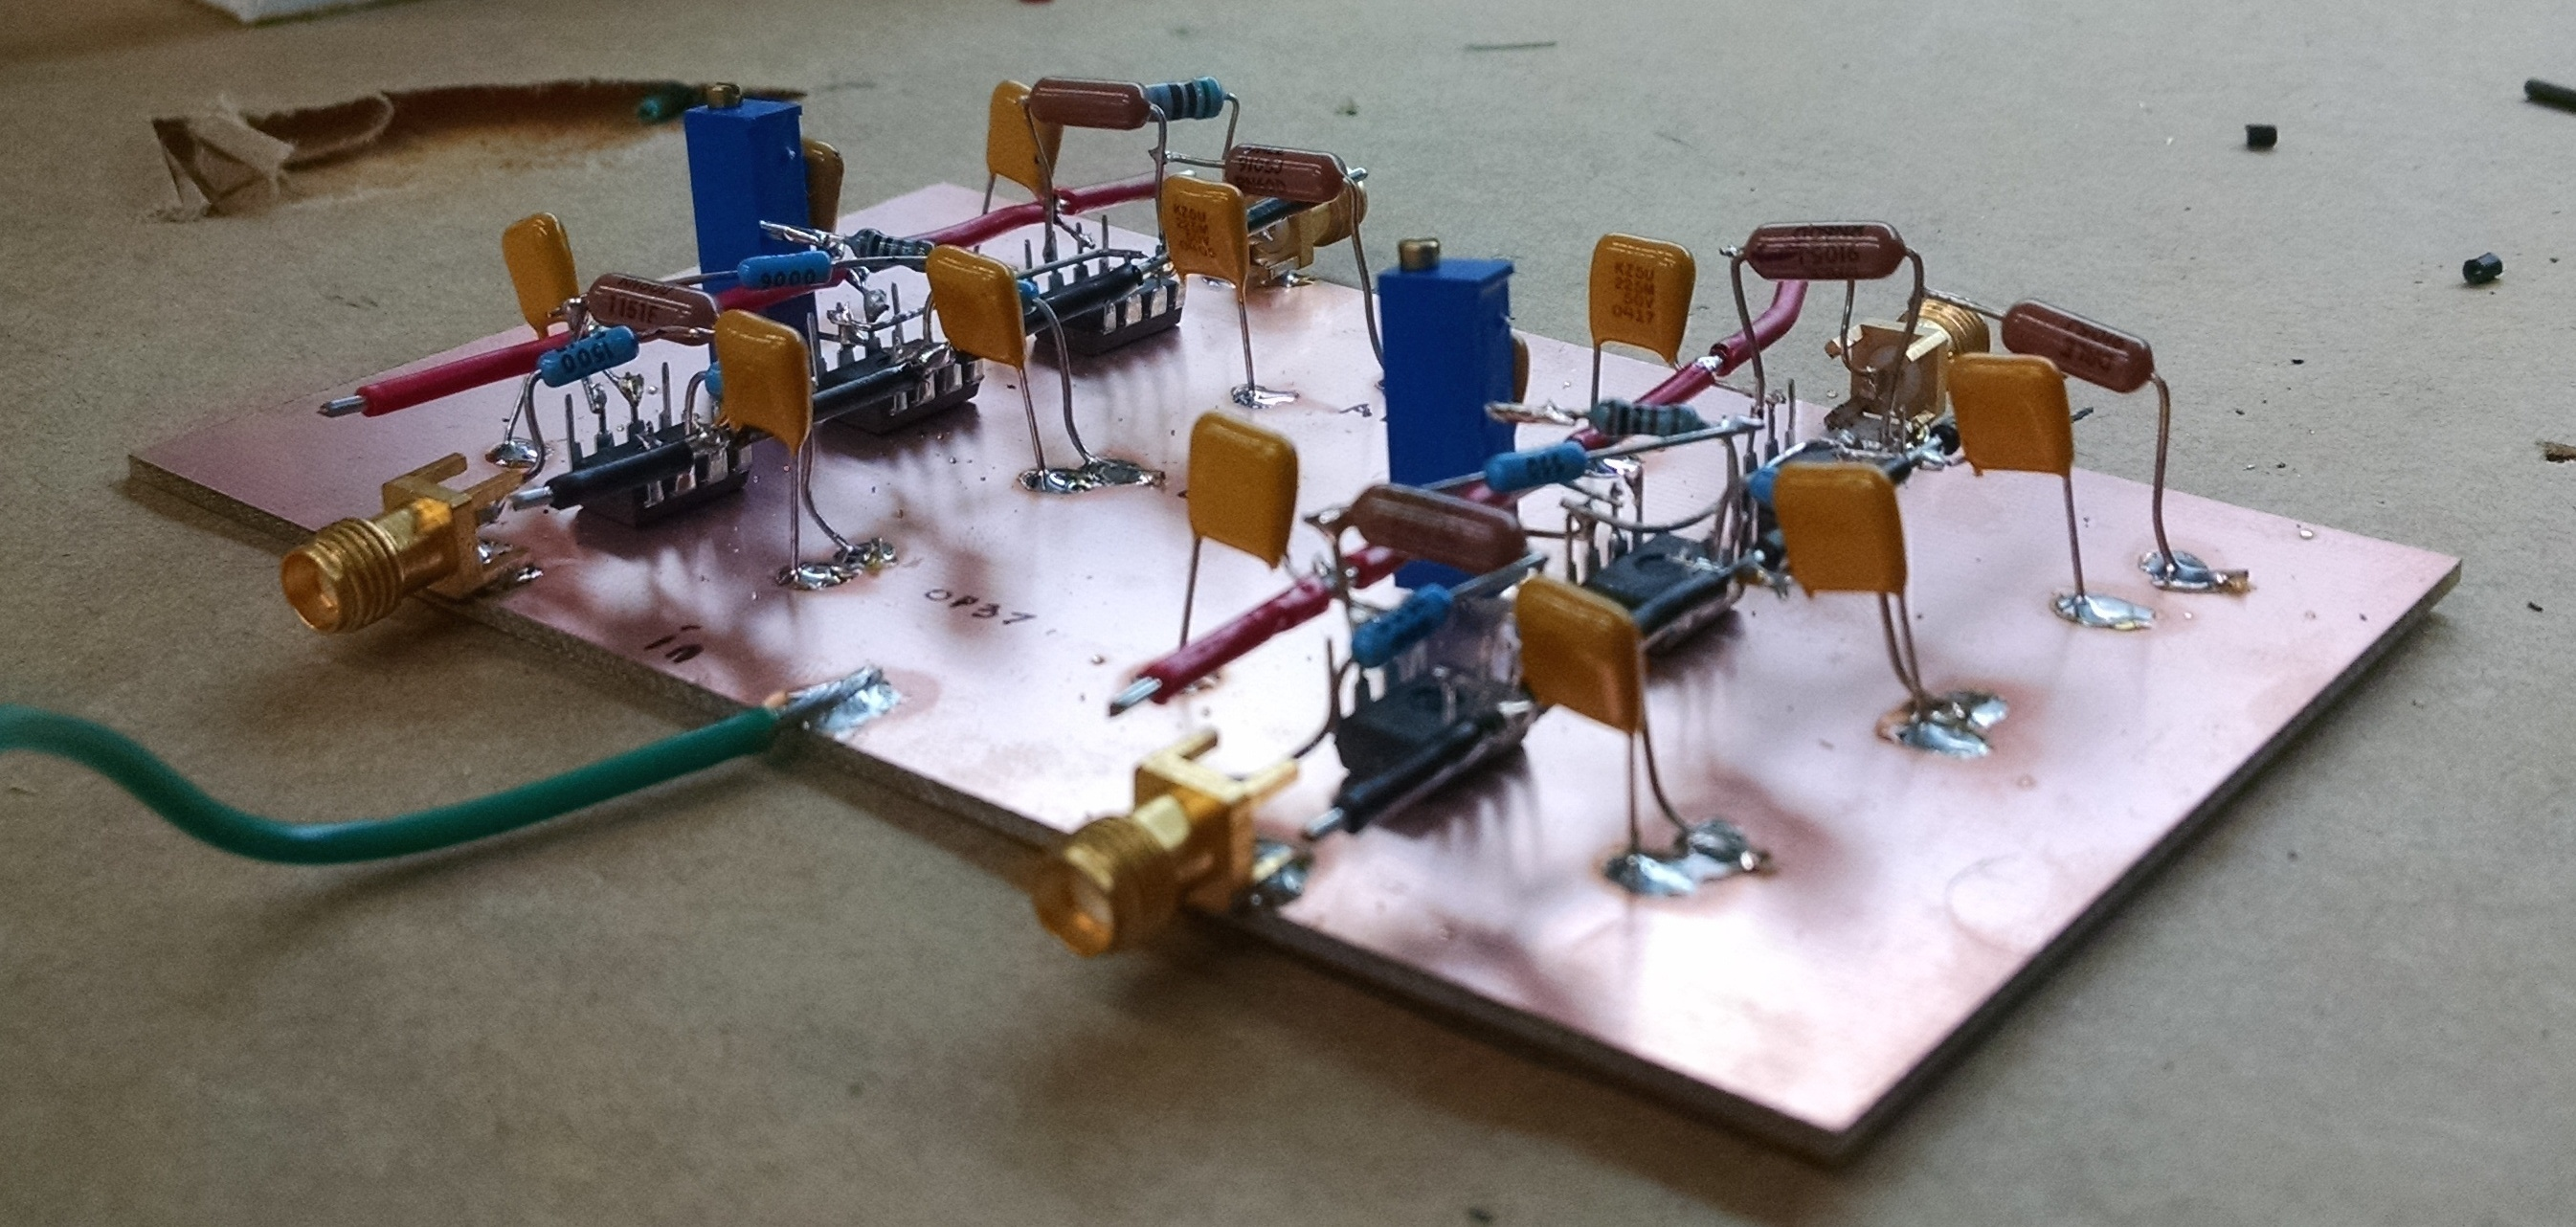
\includegraphics[width = 0.75 \textwidth]{%
    Chapters/Implementation/figs/audio_amp_picture.jpg}
  \caption[``Deadbug'' construction of audio amplifiers]{%
    The ``deadbug'' construction of the audio amplifiers
    minimizes parasitic capacitances that can produce instability.
    The operational amplifiers sit upside down,
    resembling ``dead bugs'', and
    are held in place by their solder connections
    to other components in the circuit.
    An unetched printed circuit board
    serves as the grounding plane.
    The amplifiers are packaged within a protective box
    (not pictured here).
  }
\label{fig:Implementation:audio_amplifier_picture}
\end{figure}


\subsection{Anti-aliasing filters}
\label{sec:Implementation:Hardware:anti_aliasing_filters}
Passive anti-aliasing filters
({J$3715$-$840$K-$50$-$720$B}, TTE Filters; Arcade, NY USA)
sit immediately upstream of the digitizer.
Each filter has $\SI{50}{\ohm}$ input and output impedance,
a DC to $\SI{840}{\kilo\hertz}$ passband, and
$\SI{3}{\decibel}$ frequency of just over $\SI{1}{\mega\hertz}$.
These filters are reclaimed PCI components, but
future procurement of filters with a larger passband
($\lesssim \SI{2}{\mega\hertz}$ for
typical $f_s = 4 \; \text{MSPS}$ sampling rates)
would improve the interferometer's bandwidth.


\section{Data preparation}
\label{sec:Implementation:DataPreparation}
The interferometer-measured phase $\phi_m$
is computed from the in-phase $I$ and quadrature $Q$ signals
via the two-argument arctangent function in
(\ref{eq:DesignConsiderations:summary:phase_from_arctangent}).
Before computing the measured phase $\phi_m$, however,
the ellipticity of the $I$ and $Q$ signals is compensated, as described in
Section~\ref{sec:Implementation:DataPreparation:ellipticity_compensation}.
Then, before computing the autospectral density,
a zero-delay, finite-impulse-response, high-pass filter
is applied to the measured phase $\phi_m$, as described in
Section~\ref{sec:Implementation:DataPreparation:high_pass_filtering}.


\subsection{Ellipticity compensation of $I$ \& $Q$ signals}
\label{sec:Implementation:DataPreparation:ellipticity_compensation}
Demodulator imperfections produce a relative error
in the measured fluctuating phase, as described in
Section~\ref{sec:DesignConsiderations:demodulation:imperfection_implications}.
Because the IF power entering the demodulator is sufficiently small,
demodulator nonlinearities are negligible, and
the $I$ and $Q$ signals possess negligible higher-order harmonics
(i.e.\ $|I_3| \ll I_1$, $|Q_3| \ll Q_1$, etc.).
Thus, a Lissajous figure of $Q$ from
(\ref{eq:DesignConsiderations:Q_general})
vs.\ $I$ from (\ref{eq:DesignConsiderations:I_general})
is an ellipse.
This ellipse is fitted with a direct, efficient, least-squares algorithm
\cite{fitzgibbon_ieee99,vanforeest_ellipse_fitting}.
The resulting fit is then used to compensate
any DC offsets, amplitude imbalance, and phase imbalance
in the $I$ and $Q$ signals,
minimizing the relative error
(\ref{eq:DesignConsiderations:relative_fluctuation_error})
in the measured fluctuating phase.
Fig.~\ref{fig:Implementation:ellipticity_compensation}
displays an example of raw and compensated $I$ and $Q$ signals.

\begin{figure}
  \centering
  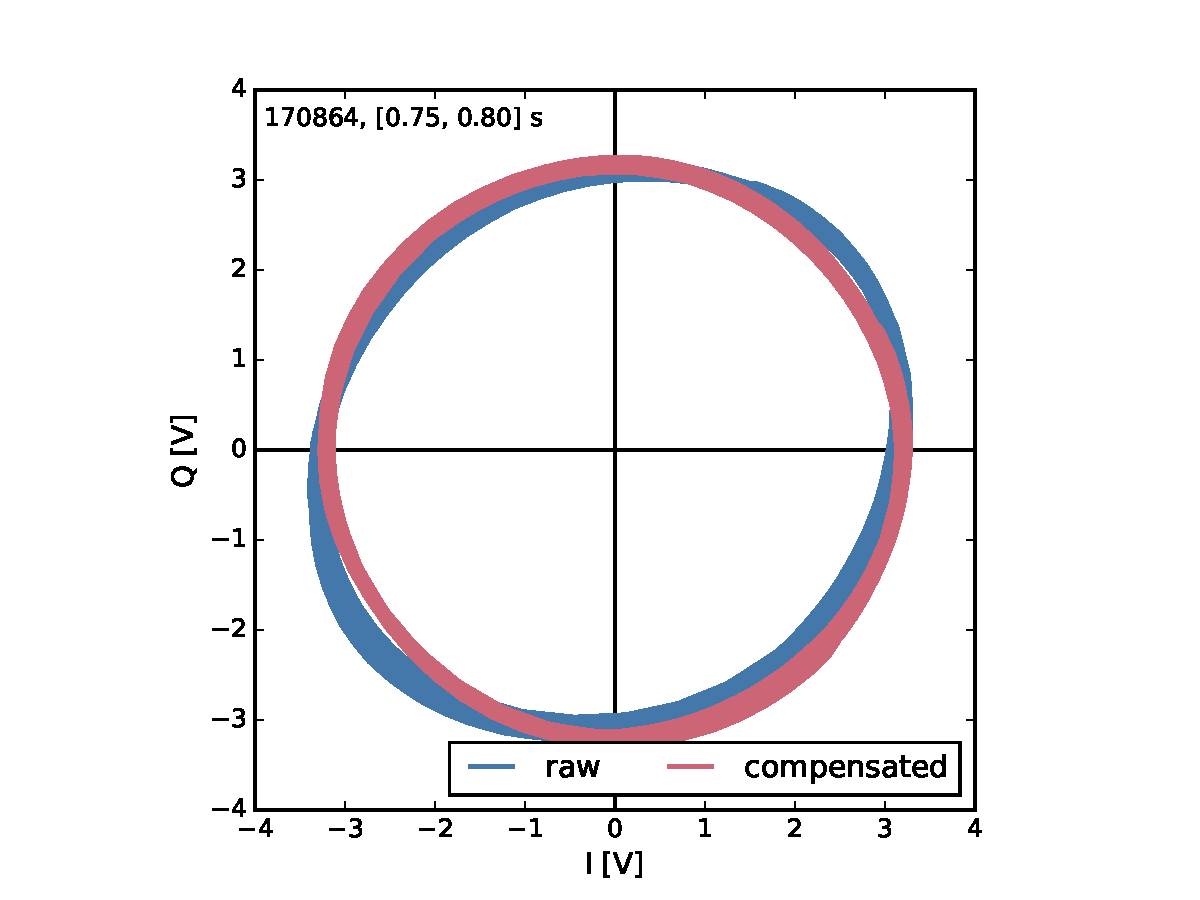
\includegraphics[width = \textwidth]{%
    Chapters/Implementation/figs/ellipticity_compensation.pdf}
  \caption[Ellipticity compensation of the $I$ and $Q$ signals]{%
    An example of the ellipticity compensation
    applied to the $I$ and $Q$ signals
    prior to computing the measured phase $\phi_m$.
  }
\label{fig:Implementation:ellipticity_compensation}
\end{figure}


\subsection{High-pass filtering the measured phase $\phi_m$}
\label{sec:Implementation:DataPreparation:high_pass_filtering}
Vibrations contaminate the low-frequency components
($f \lesssim \SI{10}{\kilo\hertz}$)
of the measured phase $\phi_m$.
At the lowest frequencies,
vibrational contributions to $\phi_m$
are orders-of-magnitude larger ($\gtrsim \SI{100}{\decibel}$)
than the corresponding plasma contribution.
Spectral estimates are often computed
after time-history tapering with a Hanning window and
with frequency resolution $\sim \SI{1}{\kilo\hertz}$.
While the Hanning window provides at least
$\SI{32}{\decibel}$ side-lobe suppression
\cite[Sec.~11.5.2.1]{bendat_and_piersol},
the vibrational component to $\phi_m$ is so large that
substantial spectral leakage can still occur.
To minimize spectral leakage, then,
the measured phase is high-pass filtered in software
to remove the large vibrational contributions.
A non-causal, type-I, finite-impulse-response (FIR) filter
has the desirable property that it produces zero delay
for all frequencies~\cite{kaiser_rsi77}\cite[Sec.~5.7.3]{oppenheim}.
Such a filter can be easily designed via
the Kaiser window method
\cite[Sec.~7.5.3]{oppenheim}\cite{scipy_kaiser_window}.
Typically, a Kaiser-designed, high-pass filter with
$\SI{-120}{\decibel}$ ripple,
$\SI{10}{\kilo\hertz}$ cut-on frequency, and
$\SI{5}{\kilo\hertz}$ width
performs sufficiently;
for the typical $f_s = 4 \; \text{MSPS}$ digitization rate,
such a filter has a length $12489$
(corresponding to $\sim \SI{3}{\milli\second}$), and
only points free from the filter's boundary effects
are included in subsequent analysis
(that is, $\sim \SI{1.5}{\milli\second}$
at the beginning and the end of the record
are lost to the filter's boundary effects).


\section{Noise in heterodyne interferometer}
\label{sec:Implementation:Noise}
The sensitivity of the heterodyne interferometer
is set by the noise in the system.
Initially, the heterodyne interferometer
was plagued by enormous noise that obscured
all but the strongest coherent plasma fluctuations.
Through substantial effort,
this noise was found to be wholly attributable to
LO phase noise and the finite coupling time of the AOM.
The theory of noise generation via this mechanism was discussed in
Section~\ref{sec:DesignConsiderations:phase_noise:LO}.
Below, Section~\ref{sec:Implementation:Noise:LO}
describes a simple, all-electrical means
of characterizing LO phase noise that, in hindsight,
would have saved a great deal of time and heartache.
This section also discusses compensation
of LO phase noise with a delay line,
an approach that was empirically found to suffer from electrical pickup
during \diiid\space operations.
Ultimately, the heterodyne-interferometer noise issues
were resolved by procuring the OCXO described in
Section~\ref{sec:Implementation:Hardware:OCXO} and
eliminating the pickup-prone delay line.
Having solved the LO phase-noise issues,
Section~\ref{sec:Implementation:Noise:interferometer}
proceeds with a spectral characterization
of the predicted and measured sources of noise
in the heterodyne interferometer and
compares the resulting noise floor
to typical plasma-fluctuation spectra.


\subsection{Quantification \& delay-line compensation of LO phase noise}
\label{sec:Implementation:Noise:LO}
\begin{figure}
  \centering
  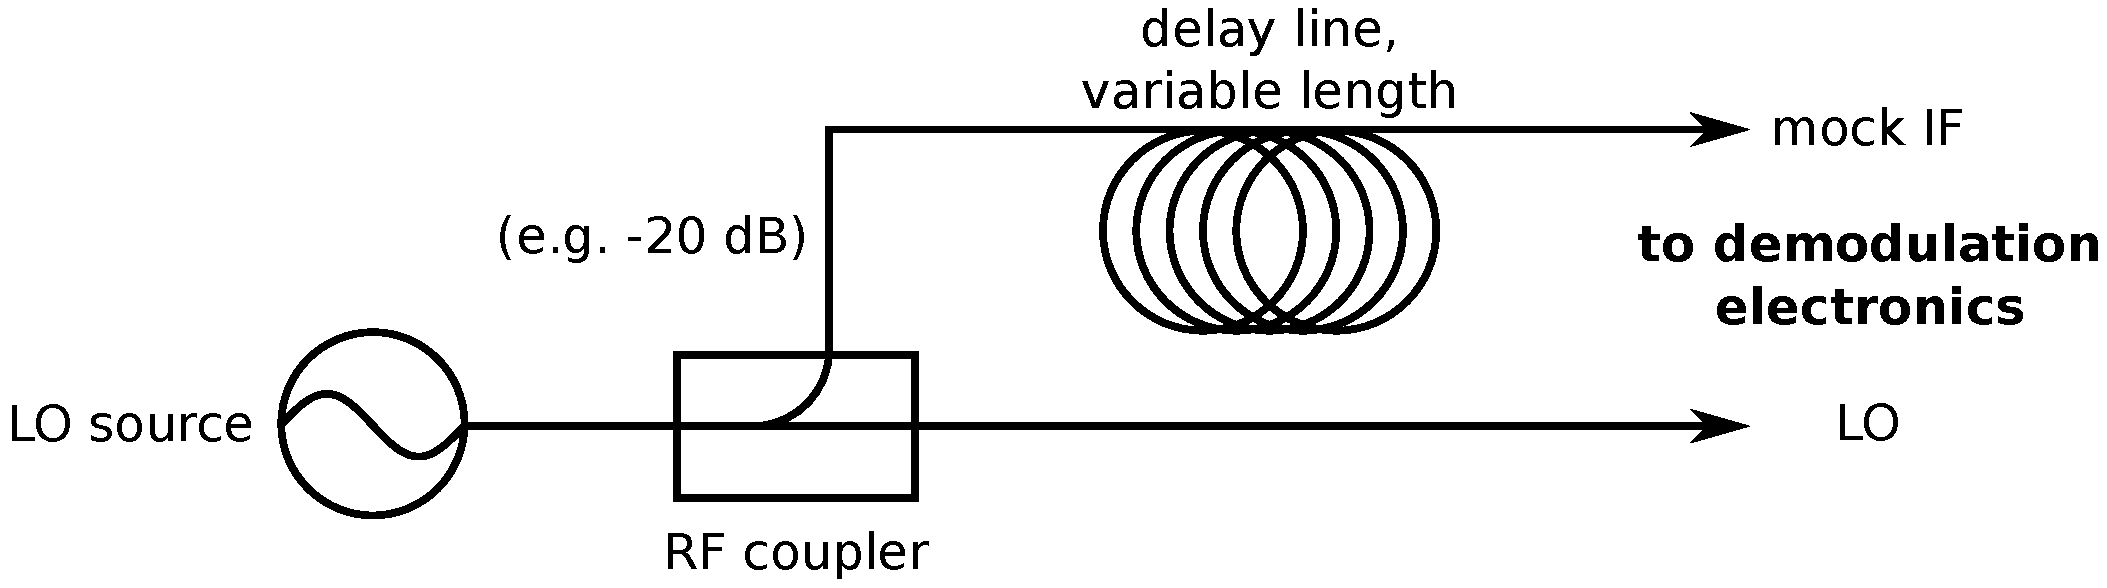
\includegraphics[width = \textwidth]{%
    Chapters/Implementation/figs/LO_self_demodulation_schematic.pdf}
  \caption[Methodology for investigating LO phase noise]{%
    Methodology for investigating LO phase noise.
  }
  \label{fig:Implementation:LO_self_demodulation_schematic}
\end{figure}

\begin{figure}
  \centering
  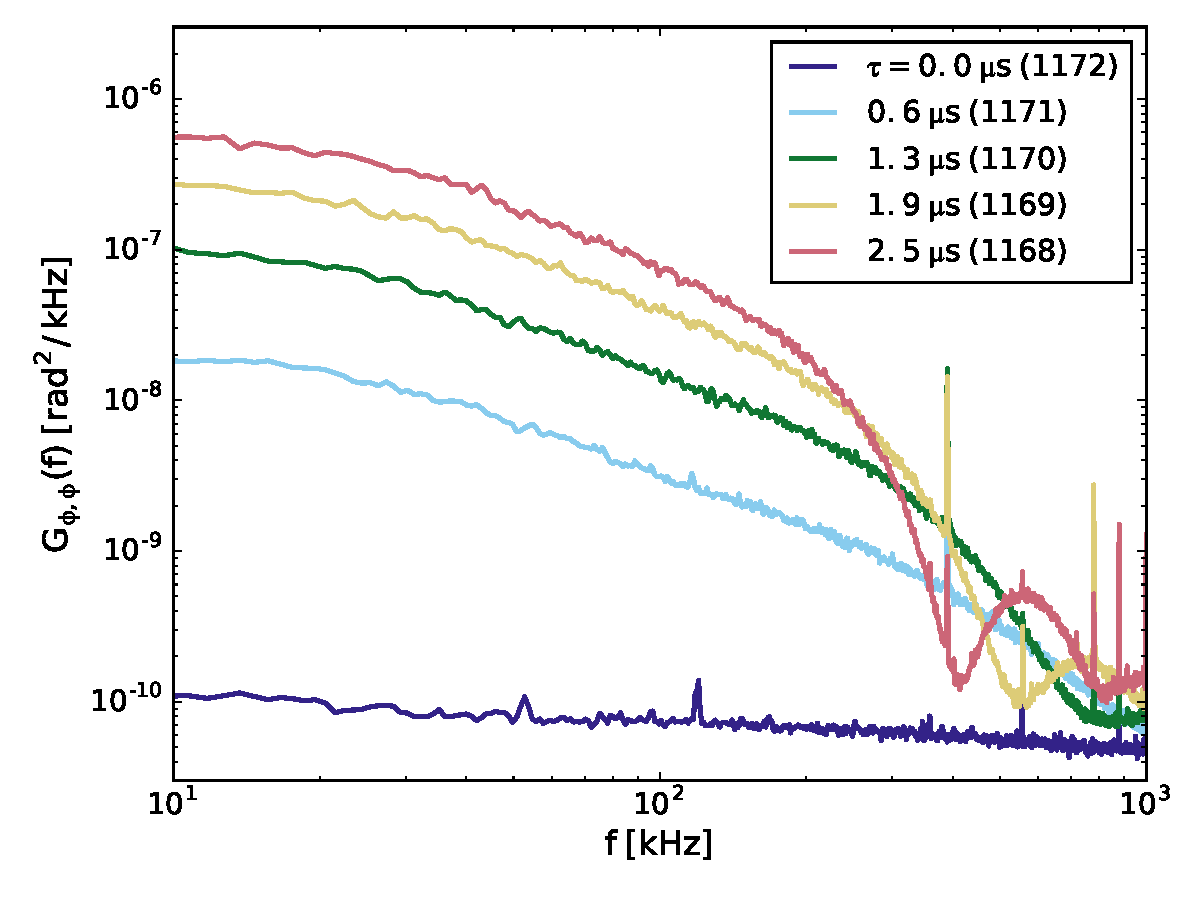
\includegraphics[width = \textwidth]{%
    Chapters/Implementation/figs/GnH_self_demodulation_varied_delay_lines.pdf}
  \caption[Coupling of XO phase noise into interferometer measurements]{%
    Coupling of XO phase noise into interferometer measurements.
  }
  \label{fig:Implementation:GnH_self_demodulation}
\end{figure}

\begin{figure}
  \centering
  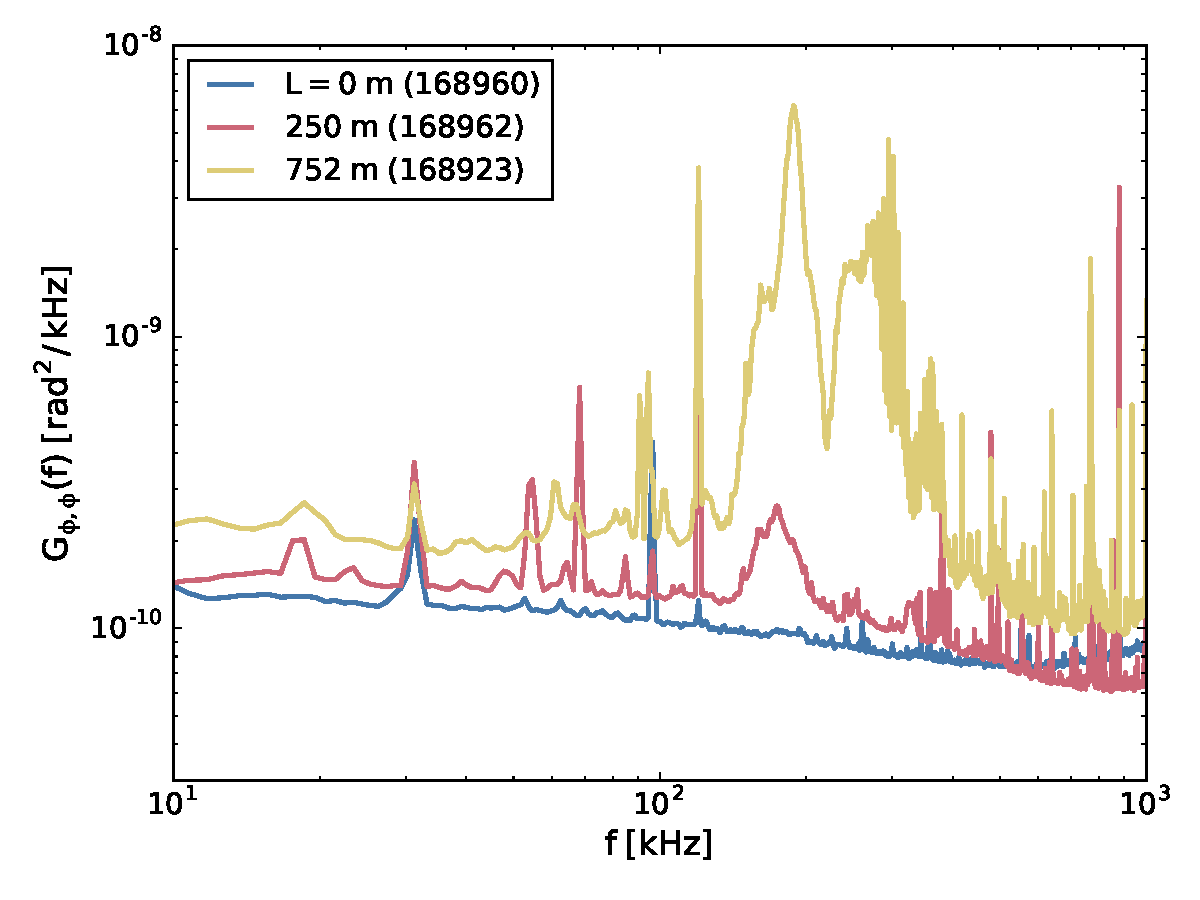
\includegraphics[width = \textwidth]{%
    Chapters/Implementation/figs/electrical_pickup.pdf}
  \caption[Delay-line electrical pickup during \diiid\space operations]{%
    Delay-line electrical pickup during \diiid\space operations.
  }
  \label{fig:Implementation:electrical_pickup}
\end{figure}


\subsection{Spectral characterization of heterodyne-interferometer noise}
\label{sec:Implementation:Noise:interferometer}
\begin{figure}
  \centering
  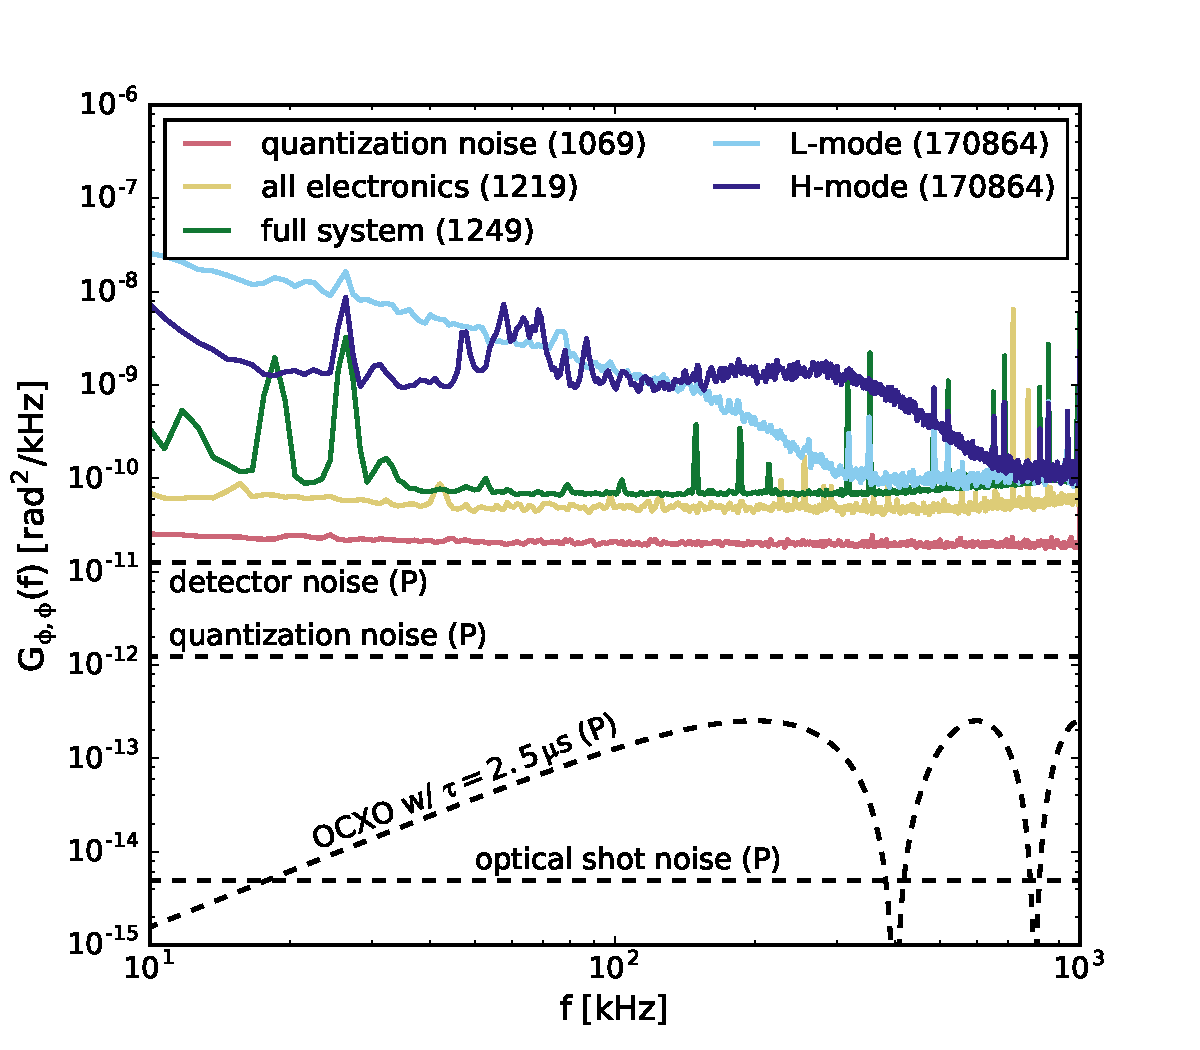
\includegraphics[width = \textwidth]{%
    Chapters/Implementation/figs/signal_and_noise.pdf}
  \caption[Spectral characterization of interferometer noise]{%
    Spectral characterization of interferometer noise and
    comparison to typical plasma-fluctuation spectra.
    Dashed lines indicate predicted (P) quantities, while
    colored traces correspond to measured quantities
    with shot numbers in parentheses
    (4 digits indicate a diagnostic test shot, and
    6 digits indicate a \diiid\space shot).
    Importantly, the interferometer noise floor
    (i.e.\ the ``full system'' trace)
    is an order of magnitude smaller than
    typical plasma fluctuations.
    Vibrations dominate the interferometer spectrum
    for $f \lesssim \SI{10}{\kilo\hertz}$.
  }
\label{fig:Implementation:signal_and_noise}
\end{figure}


\section{Alignment}
\label{sec:Implementation:Alignment}
\section{Sound-wave calibration of combined PCI-interferometer}
\subsection{Sound-wave characterization}
\subsection{Measurements}
\begin{itemize}
  \item Wavenumber range
  \item Cross calibration
  \item System sensitivity
\end{itemize}

\begin{table}[ht]
  \centering
  \renewcommand{\arraystretch}{1.5}% Spread rows out...
  \begin{tabular}{%
    >{\centering}m{3.0cm} >{\centering}m{4.5cm} >{\centering}m{4.5cm}
  }
    \toprule%
    \textbf{Parameter} & \textbf{PCI} & \textbf{Interferometer}
    \tabularnewline%
    \midrule
    \textbf{probe beam} & single CO$_2$ beam & single CO$_2$ beam
    \tabularnewline%
    \textbf{frequency bandwidth}
    & \SI{10}{\kilo\hertz} $ < f < $ \SI{2}{\mega\hertz}
    & \SI{10}{\kilo\hertz} $ < f < $ \SI{2}{\mega\hertz}
    \tabularnewline%
    \textbf{spatial bandwidth}
    & \SI{1.5}{\centi\meter}\ts{-1} $ < k < $ \SI{20}{\centi\meter}\ts{-1}
    & \SI{0}{\centi\meter}\ts{-1} $ < k < $ \SI{5}{\centi\meter}\ts{-1}
    \tabularnewline%
    \toprule%
  \end{tabular}
  \caption[Parameters of \diiid's combined PCI-interferometer]{%
    PCI and interferometry have compatible probe beams, comparable
    frequency bandwidths, and \emph{complementary} spatial bandwidths.
    All parameters are for DIII-D's currently implemented PCI--interferometer
    system.
  }%
\label{table:Implementation:PCI_interferometer}
\end{table}


% \section{Looking towards ITER\ldots}
%
%
% \section{Component replacement}
% Over the course of this work,
% several components crucial to the operation of the PCI
% (and the soon-to-be-described interferometer)
% failed.
% The failures and replacements are briefly described below.
%
%
% \subsection{Quadrature detector for beam-position feedback}
% A quadrature detector measures the position
% of the unscattered beam on the phase plate,
% providing the input to the feedback control system
% that dynamically centers the unscattered beam
% on the phase-plate groove~\cite[Sec.~3.5]{coda_phd}.
% As the quadrature detector
% cannot physically be co-located with the phase plate,
% a beam splitter samples the unscattered beam
% immediately upstream of the phase plate, and
% a single lens \emph{images} onto the quadrature detector
% the point in the sampled beam that corresponds to the phase-plate location.
% Thus, beam movement on the phase plate is mirrored
% by movement of the sampled beam on the quadrature detector.
% System response is maximized
% with imaging magnification $|M| \approx 1$
% (relative to the beam size at the phase plate) and
% incident optical intensities $I_{\text{opt}}$
% well beyond the linear saturation intensity
% (i.e. $I_{\text{sat}} \ll I_{\text{opt}} < I_{\text{dam}}$)
% ~\cite{marinoni_FB_detector_report}~\cite[Sec.~3.5(b)]{coda_phd}.
%
% The old quadrature detector consisted of four
% photoconductive, liquid-nitrogen cooled, HgCdTe elements.
% Quadrature detectors for use at $\SI{10.6}{\micro\meter}$
% had only just become commercially available
% when this unit was procured from Belov Technology in the mid-1990s
% ~\cite[Sec.~3.5(b)]{coda_phd}.
% Cooling HgCdTe can
% extend the long-wavelength cutoff beyond $\SI{10.6}{\micro\meter}$,
% reduces noise, and
% increases responsivity~\cite{vigo_catalog}.
% In particular, HgCdTe's responsivity increases by $\sim 10^3$
% when cooled to liquid-nitrogen temperatures such that
% that the incident optical signal
% exceeds the $1 / f$ noise
% characteristic of photoconductive detectors~\cite{vigo_catalog}.
% As the bandwidth requirements for the PCI feedback system
% extend from DC to $\lesssim \SI{10}{\kilo\hertz}$,
% $1 / f$ noise cannot be easily combated by
% e.g.\ mechanically chopping the beam.
% After $\sim 20$ years of operation,
% the old quadrature detector failed in December 2014,
% presumably having reached its expected lifetime.
% As Belov Technology no longer exists,
% it was not possible to procure a drop-in replacement.
% Fortunately, in the context of position sensing,
% HgCdTe technology has significantly improved since the mid-1990s.
%
% The new quadrature detector
% (four VIGO PVM-10.6 elements mounted on a VIGO QIP preamplifier)
% is in many ways superior to the old quadrature detector.
% This superiority stems from VIGO's use of
% ``multiple heterojunction'' HgCdTe detector elements~\cite{vigo_catalog},
% which endow the detector with several advantageous properties.
% First, the detector is photovoltaic.
% Thus, the detector is \emph{not} plagued by the $1 / f$ noise
% characteristic of photoconductive detectors.
% Second, the detector's long-wavelength cutoff
% sits beyond $\SI{10.6}{\micro\meter}$ at room temperature.
% Taken together, the above two properties imply that
% the new quadrature detector can be operated at room temperature,
% i.e.\ it does \emph{not} need to be cooled by liquid nitrogen.
% Lacking a dewar, the new quadrature detector
% is much smaller than the old quadrature detector;
% the new detector can also be mounted with an arbitrary orientation,
% whereas the dewar of the old detector required an upright orientation.
% This new-found flexibility substantially opened
% the optical design space for the feedback arm and
% the plasma arm of the soon-to-be-described interferometer.
% Additionally, the dewar of the old quadrature detector
% only had a $\sim \SI{6}{\hour}$ hold time,
% which is not sufficient for a full day of \diiid \space operations;
% thus, the use of a room-temperature quadrature detector has
% eliminated the mid-day ``pit runs'' to refill the quadrature detector's dewar,
% allowing easier operation of the system.
% Although room-temperature operation reduces
% the detector's specific detectivity to
% $D^* \sim \SI{e7}{\centi\meter \sqrt\hertz \per\watt}$
% (roughly three orders of magnitude \emph{lower} than
% that of the old quadrature detector),
% the optical signal corresponds to the strong, unscattered probe beam
% (as opposed to e.g.\ weak beams
% scattered from small-amplitude plasma fluctuations), so
% the increase in noise negligibly influences operation of the feedback system.
%
% \begin{itemize}
%   \item When was new detector acquired?
%   \item \textcolor{red}{Picture}
%   \item \textcolor{red}{Table of properties (?)}
% \end{itemize}
%
%
% \subsection{CO$_2$ laser}
% The old CO$_2$ laser~\cite[Sec.~3.3]{coda_phd},
% manufactured by MPB Technologies,
% had been in service since
% the inception of the \diiid \space PCI system in the mid-1990s.
% Lasing occurred via high voltage, DC-excitation
% inside of a $\SI{2}{\meter}$-long, sealed-off glass tube
% to produce a TEM$_{00}$ (Gaussian) mode with linear polarization.
% The laser nominally had
% a $\lesssim \SI{300}{\kilo\hertz}$ frequency stability
% over short time windows ($\SI{0.1}{\second}$) and
% a $\lesssim \SI{3}{\mega\hertz}$ frequency stability
% over longer time windows ($\SI{e3}{\second}$).
% The laser's tube was replaced in late 1999
% when a precipitous drop in beam power indicated imminent failure.
% Following the tube's replacement,
% the measured beam power consistently hovered at $\sim\SI{14}{\watt}$
% for many years.
% However, in early 2016, the beam power again precipitously dropped.
% The laser's high voltage power supply,
% which was replaced in 2005 after failing,
% was tested and found to be operating nominally,
% suggesting that the drop in beam power
% was attributable to the laser's aging tube.
% Unfortunately, MPB Technologies has abandoned its efforts in CO$_2$ lasers
% and was unable to replace or repair the tube.
% Third-party tube repair was investigated but
% ultimately deemed unacceptable due to
% the required lead times and the lack of a guaranteed repair.
% Fortunately, the MPB laser continued operating, albeit at reduced power,
% throughout the 2016 campaign, allowing continued diagnostic development
% of the soon-to-be-described interferometer.
%
% After an exhaustive search of the CO$_2$-laser market,
% a water-cooled AL30ST CO$_2$ laser was procured
% from Access Laser Company (Everett, WA) in mid-2016.
% Lasing occurs via RF excitation at $\SI{40.68}{\mega\hertz}$;
% RF excitation requires far-lower voltages than DC excitation,
% eliminating the high-voltage safety risk and allowing more efficient lasing
% \cite{he_jap83}.
% As in the old MPB laser,
% the lasing cavity is supported by carbon fiber rods (rather than Invar)
% to mitigate any effects of the tokamak's large, ambient magnetic fields
% on the laser's performance.
% The laser oscillates on a TEM$_{00}$ (Gaussian) mode (spec'd $M^2 < 1.1$)
% with vertical polarization (spec'd extinction ratio $1 / 897$), and
% its $\SI{37}{\watt}$ power output is stable to within $\pm 1.1\%$
% \cite{marinoni_AL30ST_report}.
% Lasing occurs on the $P(20)$ line
% of the $00^{\circ}1 \rightarrow 10^{\circ}0$ transition
% to produce radiation with a vacuum wavelength of
% $\lambda_0 = \SI{10.591}{\micro\meter}$.
% Measurements with wavelength meter 621B
% from Bristol Instruments, Inc. (Victor, NY)
% indicate that the laser's wavelength stability over several seconds
% is characterized by a Voigt distribution with
% full width at half maximum of $\SI{0.0029}{\nano\meter}$, which
% corresponds to a frequency stability (over \emph{several seconds})
% of $\SI{3.8}{\mega\hertz}$ \cite{marinoni_AL30ST_report}.
%
% In the context of measuring plasma-density fluctuations
% with an external reference-beam interferometer,
% the relevant metric is the laser's frequency stability
% over much shorter time windows
% (i.e.\ the time difference corresponding to
% the difference in optical path length between
% the interferometer's plasma and reference arms).
% This is most easily evaluated empirically
% by deploying the laser in the given interferometric system
% and evaluating the corresponding phase noise.
% Successive test shots,
% the first with the old MPB laser and the second with the AL30ST,
% show comparable phase noise (and hence frequency stability)
% between the two lasers.
% Thus, the AL30ST frequency stability is deemed to be sufficient
% for measurement of plasma-density fluctuations
% with the soon-to-be-described external reference-beam interferometer.
%
% \begin{itemize}
%   \item \textcolor{red}{Picture}
%   \item \textcolor{red}{Fig. of new vs.\ old laser stability}
% \end{itemize}
%
%
% \subsection{In-vessel mirrors}
% Two of the PCI mirrors are located
% \emph{inside} of the \diiid \space vacuum vessel.
% As indicated in Fig.~\ref{fig:Implementation:d3d_port_locations}(b),
% the PCI probe beam enters the machine through the $285^{\circ}$ R+2 port,
% reflects off of the first in-vessel mirror,
% propagates vertically downwards through the machine (and the plasma),
% reflects off the second in-vessel mirror, and
% exits the machine through the $285^{\circ}$ R-2 port.
% The in-vessel mirrors are elongated
% along the axis parallel to the plane of incidence
% in order to increase the mirrors' apparent surface area.
% The mirrors were fabricated by Esco Optics, Inc. (Oak Ridge, NJ).
% The mirrors are made of fused quartz with
% a reflective aluminum surface and a protective SiO coating.
%
% In mid-2015 the beam quality of the CO$_2$ laser and the HeNe alignment laser
% after passing through the \diiid \space vessel was noted to be poor
% (i.e. substantially non-Gaussian).
% Numerous tests suggested that the poor beam quality was attributable
% damaged in-vessel mirrors;
% this hypothesis was confirmed via visual inspection
% during the next manned entry of the machine.
% ``Drop-in'' replacements were ordered from Esco Optics
% and were installed in mid-2016.
% The removed, damaged mirrors are shown in
% Fig.~\ref{fig:Implementation:in_vessel_mirrors}.
% It is not known whether the mirrors were damaged
% during e.g. plasma operations or high-temperature bakes of the vessel.
%
% \begin{figure}
%   \centering
%   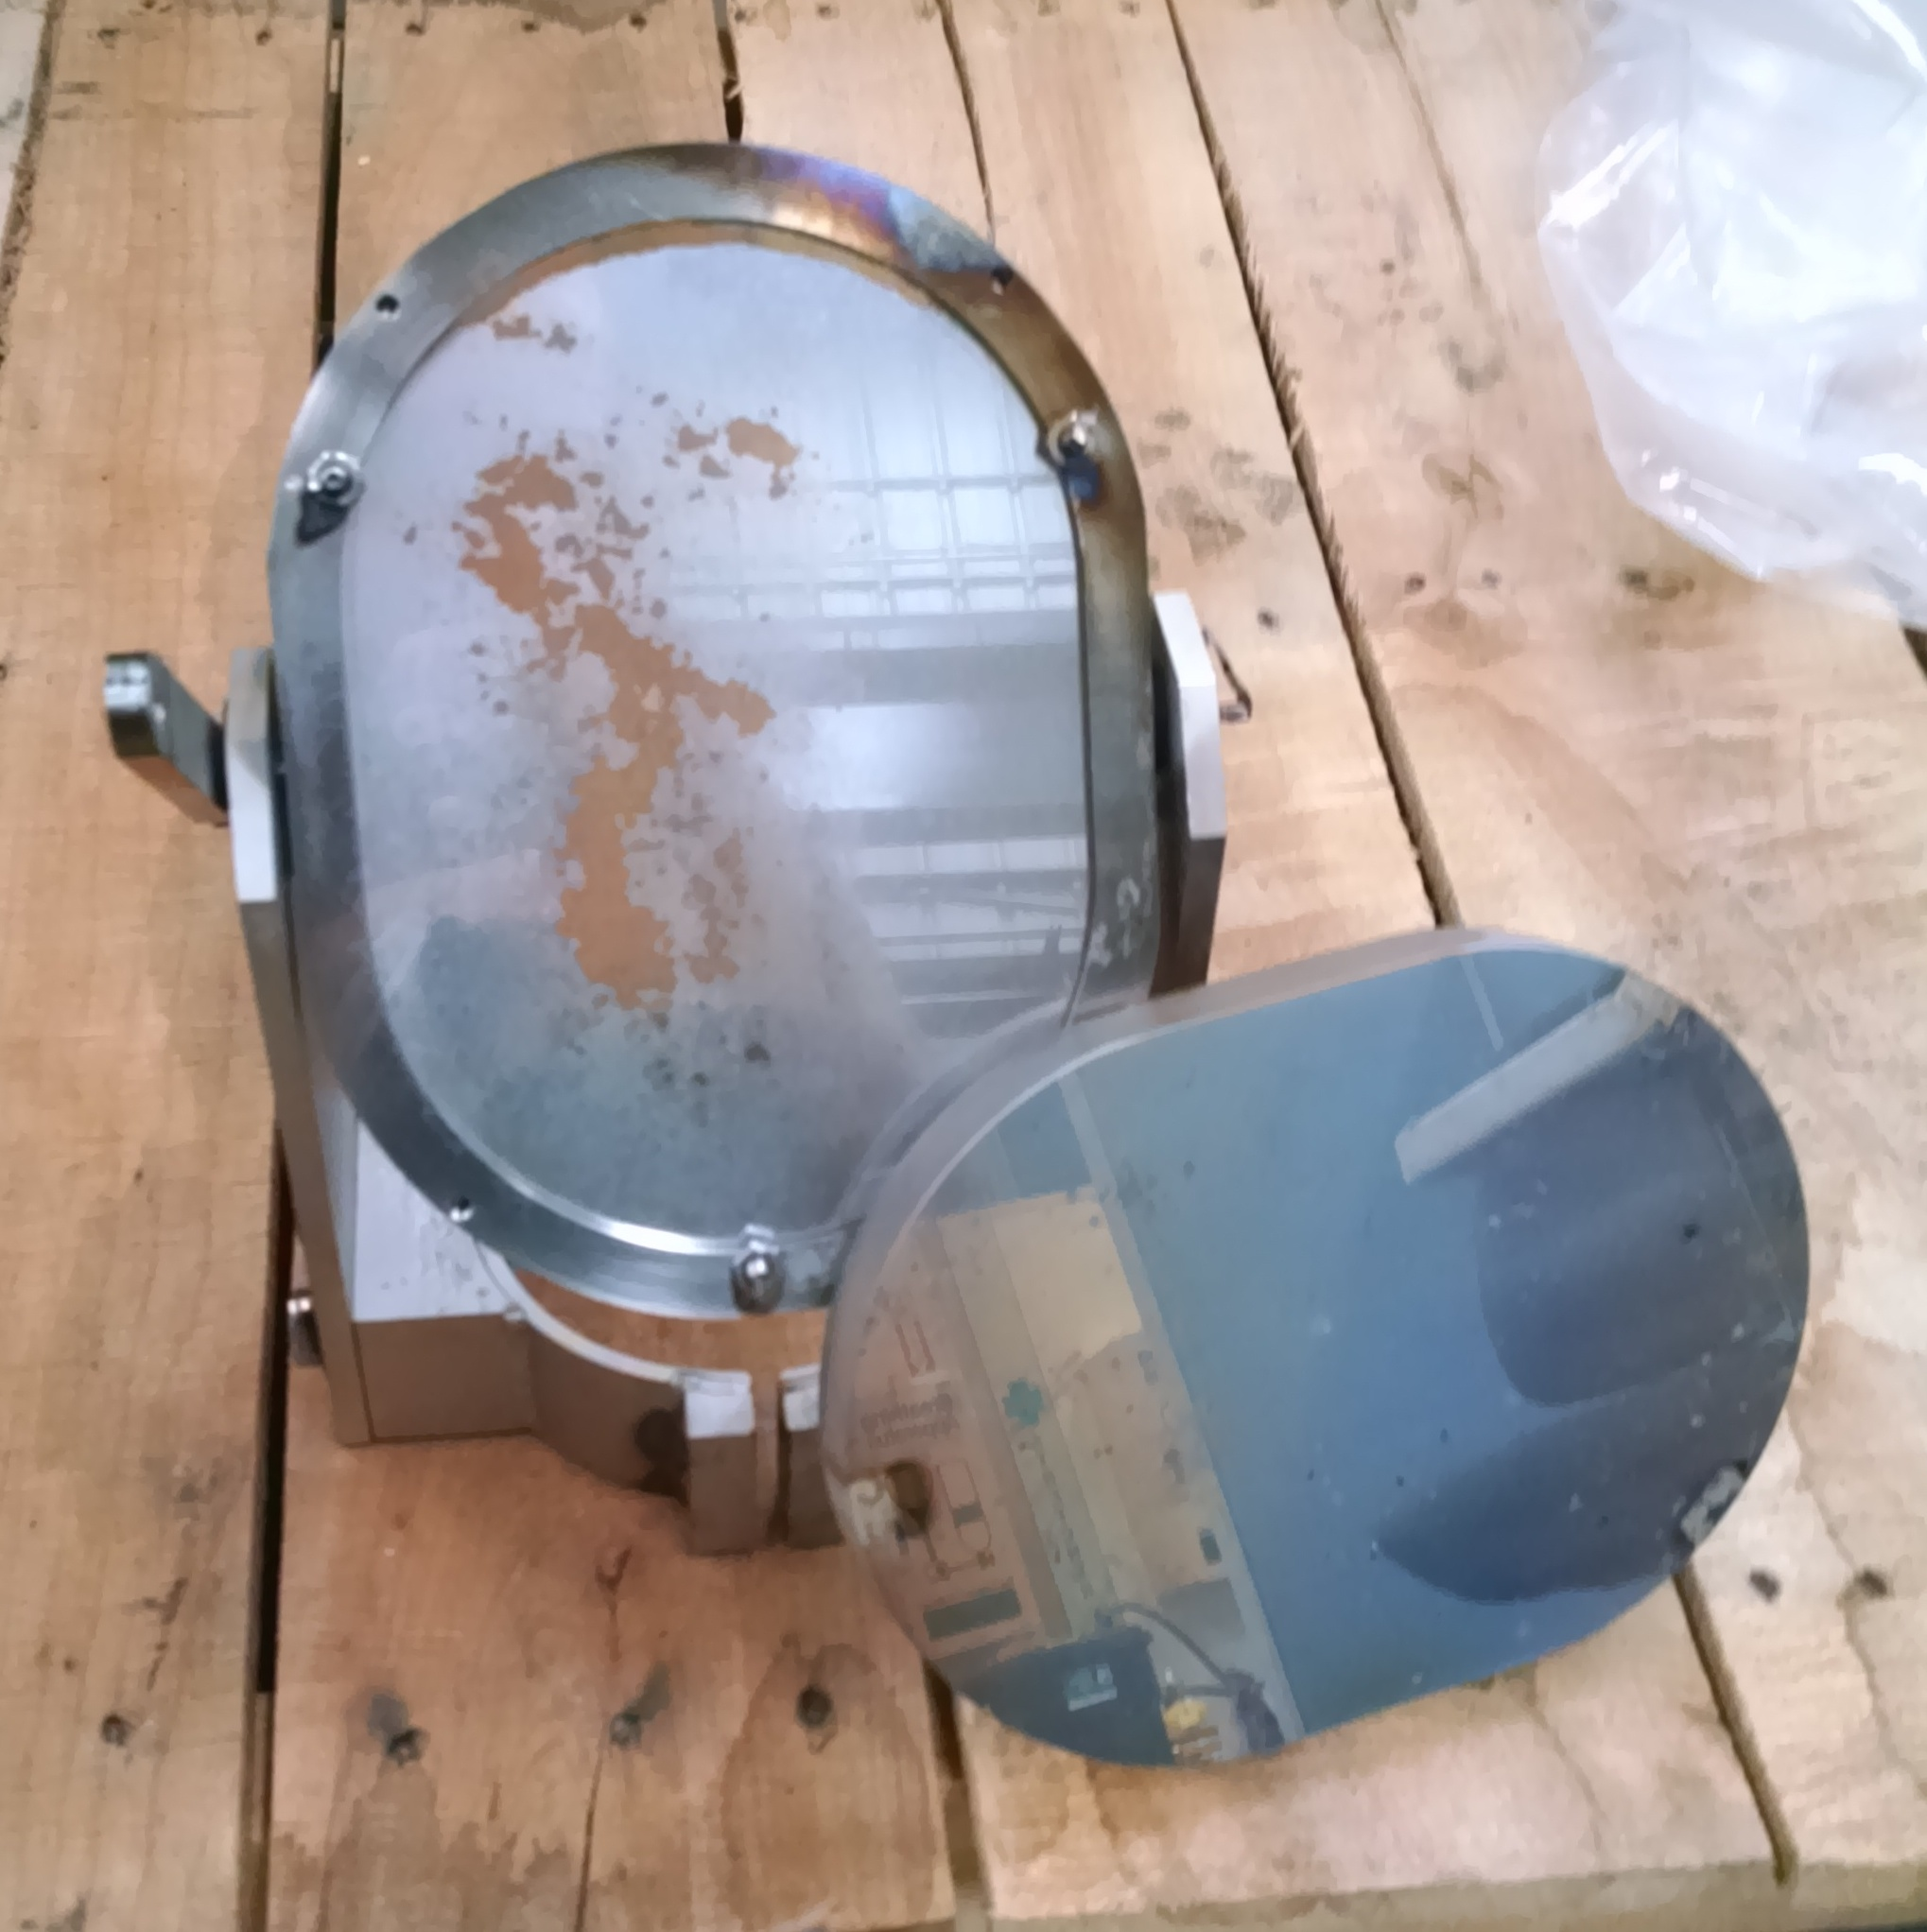
\includegraphics[width = 0.6 \textwidth]{%
%     Chapters/Implementation/figs/in_vessel_mirrors.jpg}
%   \caption[PCI's damaged in-vessel mirrors]{%
%     PCI's damaged in-vessel mirrors, sitting
%     in the \diiid \space ``Hi-Bay''
%     after removal from the vessel in mid-2016.
%     (Note that the reflectivity of each mirror at $\SI{10.6}{\micro\meter}$
%     cannot be gauged from this photograph in the visible spectrum).
%     ``Drop-in'' replacements were installed
%     before the resumption of plasma operations.}
% \label{fig:Implementation:in_vessel_mirrors}
% \end{figure}


\bibliographystyle{plainurl}
\bibliography{references}
